\chapter{Monte Carlo: Drawing Samples on a Deterministic Machine}\label{ch:06}

\providecommand{\SixAMontyN}{}\renewcommand{\SixAMontyN}{300{,}000}
\providecommand{\SixAMontyGoodLikA}{}\renewcommand{\SixAMontyGoodLikA}{0.500}
\providecommand{\SixAMontyGoodLikB}{}\renewcommand{\SixAMontyGoodLikB}{1.000}
\providecommand{\SixAMontyGoodPostA}{}\renewcommand{\SixAMontyGoodPostA}{0.333}
\providecommand{\SixAMontyGoodPostB}{}\renewcommand{\SixAMontyGoodPostB}{0.667}
\providecommand{\SixAMontyBadOneLikA}{}\renewcommand{\SixAMontyBadOneLikA}{0.000}
\providecommand{\SixAMontyBadOnePostA}{}\renewcommand{\SixAMontyBadOnePostA}{0.000}
\providecommand{\SixAMontyBadOnePostB}{}\renewcommand{\SixAMontyBadOnePostB}{1.000}
\providecommand{\SixAMontyBadTwoLikA}{}\renewcommand{\SixAMontyBadTwoLikA}{1.000}
\providecommand{\SixAMontyBadTwoPostB}{}\renewcommand{\SixAMontyBadTwoPostB}{0.501}
\providecommand{\SixAMontyGoodSwitch}{}\renewcommand{\SixAMontyGoodSwitch}{0.667}
\providecommand{\SixAMontyBadOneSwitch}{}\renewcommand{\SixAMontyBadOneSwitch}{0.667}
\providecommand{\SixAMontyBadTwoSwitch}{}\renewcommand{\SixAMontyBadTwoSwitch}{0.667}
\providecommand{\SixAPiLcgEst}{}\renewcommand{\SixAPiLcgEst}{3.0899}
\providecommand{\SixAPiLcgSe}{}\renewcommand{\SixAPiLcgSe}{0.0017}
\providecommand{\SixAPiLcgErr}{}\renewcommand{\SixAPiLcgErr}{-0.0517}
\providecommand{\SixAPiPcgEst}{}\renewcommand{\SixAPiPcgEst}{3.1389}
\providecommand{\SixAPiPcgSe}{}\renewcommand{\SixAPiPcgSe}{0.0016}
\providecommand{\SixAPiPcgErr}{}\renewcommand{\SixAPiPcgErr}{-0.0027}
\providecommand{\SixAMidSqMaxSteps}{}\renewcommand{\SixAMidSqMaxSteps}{111}
\providecommand{\SixAMidSqMeanSteps}{}\renewcommand{\SixAMidSqMeanSteps}{43.7}
\providecommand{\SixAMidSqZero}{}\renewcommand{\SixAMidSqZero}{1968}
\providecommand{\SixAMidSqZeroPct}{}\renewcommand{\SixAMidSqZeroPct}{20}
\providecommand{\SixALamAPeriod}{}\renewcommand{\SixALamAPeriod}{2048}
\providecommand{\SixALamBPeriod}{}\renewcommand{\SixALamBPeriod}{244944}
\providecommand{\SixABitPerZero}{}\renewcommand{\SixABitPerZero}{2}
\providecommand{\SixABitPerOne}{}\renewcommand{\SixABitPerOne}{4}
\providecommand{\SixABitPerTwo}{}\renewcommand{\SixABitPerTwo}{8}
\providecommand{\SixABitPerThree}{}\renewcommand{\SixABitPerThree}{16}
\providecommand{\SixABitPerEleven}{}\renewcommand{\SixABitPerEleven}{4096}
\providecommand{\SixARanduNplanes}{}\renewcommand{\SixARanduNplanes}{15}
\providecommand{\SixARanduKmin}{}\renewcommand{\SixARanduKmin}{-5}
\providecommand{\SixARanduKmax}{}\renewcommand{\SixARanduKmax}{9}
\providecommand{\SixARanduAzEdge}{}\renewcommand{\SixARanduAzEdge}{56.3}
\providecommand{\SixASpecRanduThreeNu}{}\renewcommand{\SixASpecRanduThreeNu}{10.86}
\providecommand{\SixASpecRanduThreeD}{}\renewcommand{\SixASpecRanduThreeD}{0.092}
\providecommand{\SixASpecRanduTwoD}{}\renewcommand{\SixASpecRanduTwoD}{2.158\times10^{-5}}
\providecommand{\SixASpecMinstdTwoD}{}\renewcommand{\SixASpecMinstdTwoD}{5.950\times10^{-5}}
\providecommand{\SixASpecMinstdThreeD}{}\renewcommand{\SixASpecMinstdThreeD}{0.001565}
\providecommand{\SixASpecRanduThreeIdeal}{}\renewcommand{\SixASpecRanduThreeIdeal}{6.905\times10^{-4}}
\providecommand{\SixASpecLecTwoD}{}\renewcommand{\SixASpecLecTwoD}{2.457\times10^{-5}}
\providecommand{\SixASpecLamTwoNu}{}\renewcommand{\SixASpecLamTwoNu}{5.10}
\providecommand{\SixASpecLamTwoH}{}\renewcommand{\SixASpecLamTwoH}{(1,-5)}
\providecommand{\SixASpecMinstdSixD}{}\renewcommand{\SixASpecMinstdSixD}{0.03343}
\providecommand{\SixAMarsBoundThree}{}\renewcommand{\SixAMarsBoundThree}{2954}
\providecommand{\SixAMarsBoundTen}{}\renewcommand{\SixAMarsBoundTen}{42}
\providecommand{\SixAPcgSame}{}\renewcommand{\SixAPcgSame}{100{,}000}
\providecommand{\SixAMtSame}{}\renewcommand{\SixAMtSame}{10{,}000}
\providecommand{\SixAMtPred}{}\renewcommand{\SixAMtPred}{1{,}000}
\providecommand{\SixAPairsLcg}{}\renewcommand{\SixAPairsLcg}{40{,}960}
\providecommand{\SixAPairsPcg}{}\renewcommand{\SixAPairsPcg}{41{,}488}
\providecommand{\SixAPairsLcgPct}{}\renewcommand{\SixAPairsLcgPct}{62.5}
\providecommand{\SixAPairsPcgPct}{}\renewcommand{\SixAPairsPcgPct}{63.3}
\providecommand{\SixASeedInt}{}\renewcommand{\SixASeedInt}{16002383964210800950}
\providecommand{\SixAStreamMaxCorr}{}\renewcommand{\SixAStreamMaxCorr}{0.0032}
\providecommand{\SixAStreamInvSqrtN}{}\renewcommand{\SixAStreamInvSqrtN}{0.0010}
\providecommand{\SixAStreamZstd}{}\renewcommand{\SixAStreamZstd}{1.10}
\providecommand{\SixAStreamKsP}{}\renewcommand{\SixAStreamKsP}{0.28}
\providecommand{\SixABdayThree}{}\renewcommand{\SixABdayThree}{0.0001}
\providecommand{\SixABdayFour}{}\renewcommand{\SixABdayFour}{0.012}
\providecommand{\SixABdayFive}{}\renewcommand{\SixABdayFive}{0.688}
\providecommand{\SixABdayFiveApprox}{}\renewcommand{\SixABdayFiveApprox}{0.688}
\providecommand{\SixABdayOneTwoEight}{}\renewcommand{\SixABdayOneTwoEight}{1.469\times10^{-29}}
\providecommand{\SixATPcgHistStat}{}\renewcommand{\SixATPcgHistStat}{69.93}
\providecommand{\SixATPcgHistP}{}\renewcommand{\SixATPcgHistP}{0.256}
\providecommand{\SixATPcgSerStat}{}\renewcommand{\SixATPcgSerStat}{-0.69}
\providecommand{\SixATPcgSerP}{}\renewcommand{\SixATPcgSerP}{0.493}
\providecommand{\SixATPcgRunsStat}{}\renewcommand{\SixATPcgRunsStat}{1.84}
\providecommand{\SixATPcgRunsP}{}\renewcommand{\SixATPcgRunsP}{0.066}
\providecommand{\SixATPcgTriStat}{}\renewcommand{\SixATPcgTriStat}{7748}
\providecommand{\SixATPcgTriP}{}\renewcommand{\SixATPcgTriP}{0.977}
\providecommand{\SixATMtHistStat}{}\renewcommand{\SixATMtHistStat}{69.53}
\providecommand{\SixATMtHistP}{}\renewcommand{\SixATMtHistP}{0.267}
\providecommand{\SixATMtSerStat}{}\renewcommand{\SixATMtSerStat}{-0.40}
\providecommand{\SixATMtSerP}{}\renewcommand{\SixATMtSerP}{0.693}
\providecommand{\SixATMtRunsStat}{}\renewcommand{\SixATMtRunsStat}{0.16}
\providecommand{\SixATMtRunsP}{}\renewcommand{\SixATMtRunsP}{0.873}
\providecommand{\SixATMtTriStat}{}\renewcommand{\SixATMtTriStat}{8144}
\providecommand{\SixATMtTriP}{}\renewcommand{\SixATMtTriP}{0.126}
\providecommand{\SixATRanduHistStat}{}\renewcommand{\SixATRanduHistStat}{46.66}
\providecommand{\SixATRanduHistP}{}\renewcommand{\SixATRanduHistP}{0.939}
\providecommand{\SixATRanduSerStat}{}\renewcommand{\SixATRanduSerStat}{-0.49}
\providecommand{\SixATRanduSerP}{}\renewcommand{\SixATRanduSerP}{0.624}
\providecommand{\SixATRanduRunsStat}{}\renewcommand{\SixATRanduRunsStat}{1.02}
\providecommand{\SixATRanduRunsP}{}\renewcommand{\SixATRanduRunsP}{0.306}
\providecommand{\SixATRanduTriStat}{}\renewcommand{\SixATRanduTriStat}{2.473\times10^{5}}
\providecommand{\SixATRanduTriP}{}\renewcommand{\SixATRanduTriP}{<10^{-300}}
\providecommand{\SixATLamHistStat}{}\renewcommand{\SixATLamHistStat}{0.02259}
\providecommand{\SixATLamHistP}{}\renewcommand{\SixATLamHistP}{1.000}
\providecommand{\SixATLamSerStat}{}\renewcommand{\SixATLamSerStat}{197.09}
\providecommand{\SixATLamSerP}{}\renewcommand{\SixATLamSerP}{<10^{-300}}
\providecommand{\SixATLamRunsStat}{}\renewcommand{\SixATLamRunsStat}{-156.69}
\providecommand{\SixATLamRunsP}{}\renewcommand{\SixATLamRunsP}{<10^{-300}}
\providecommand{\SixATLamTriStat}{}\renewcommand{\SixATLamTriStat}{4.870\times10^{6}}
\providecommand{\SixATLamTriP}{}\renewcommand{\SixATLamTriP}{<10^{-300}}
\providecommand{\SixATLamHistLowP}{}\renewcommand{\SixATLamHistLowP}{9.9\times10^{-97}}
\providecommand{\SixATreps}{}\renewcommand{\SixATreps}{400}
\providecommand{\SixATksP}{}\renewcommand{\SixATksP}{0.36}
\providecommand{\SixAEmptyPcg}{}\renewcommand{\SixAEmptyPcg}{92}
\providecommand{\SixAEmptySobol}{}\renewcommand{\SixAEmptySobol}{0}
\providecommand{\SixAEmptyExpected}{}\renewcommand{\SixAEmptyExpected}{94}
\providecommand{\SixASlopeSmoothMc}{}\renewcommand{\SixASlopeSmoothMc}{-0.51}
\providecommand{\SixASlopeSmoothSob}{}\renewcommand{\SixASlopeSmoothSob}{-1.08}
\providecommand{\SixASlopeBallMc}{}\renewcommand{\SixASlopeBallMc}{-0.51}
\providecommand{\SixASlopeBallSob}{}\renewcommand{\SixASlopeBallSob}{-0.57}
\providecommand{\SixAGainSmooth}{}\renewcommand{\SixAGainSmooth}{135}
\providecommand{\SixAGainBall}{}\renewcommand{\SixAGainBall}{2.5}
\providecommand{\SixASobolR}{}\renewcommand{\SixASobolR}{40}
\providecommand{\SixABallVol}{}\renewcommand{\SixABallVol}{0.1645}
 
\section*{Where this chapter is going}
\label{6a:sec:roadmap}

Every simulation in this book starts the same way: a line such as
\texttt{rng.random(N)} hands us $N$ numbers that behave like independent draws
from the uniform distribution on $[0,1)$. From them we build draws from any
distribution we like, and averages over the draws estimate probabilities,
expectation values and integrals that no formula gives us. The computer that
produces those numbers is a deterministic machine: run the same program twice and
it does exactly the same thing. So the numbers cannot be random. They are the
output of a small dynamical system, a \emph{state} that is updated by a fixed
rule, and the only honest claim we can make about them is a statistical one: no
test we care about can tell them apart from genuinely independent uniform draws.

That claim can fail, and it has failed in instructive ways. A generator has a
finite number of states, so it must eventually repeat, and after that no new
information enters a simulation. The simplest generators, the linear
congruential ones, put their consecutive outputs on a crystal lattice: in three
dimensions the triples of IBM's famous RANDU lie on just fifteen planes. Their
lowest bits repeat with tiny periods. Modern generators (xorshift, the Mersenne
Twister, and numpy's default PCG64) keep a larger state, update it by a rule that
is cheap and has an enormous period, and pass it through an output function that
hides the regularities the update leaves behind. Seeds and streams let us rerun
any simulation bit for bit and run thousands of independent copies side by side.
Whether a generator is good enough is a hypothesis test: $H_0$ is ``independent
and uniform'', and the test statistics are histograms, correlations, runs and
tuples. Finally, when the goal is an integral rather than a random process, we
may drop randomness altogether: quasi-random points fill space more evenly than
independent points and beat the $1/\sqrt N$ error.

From uniform numbers we then build draws from any distribution (inverse
transform, Box--Muller, rejection and importance sampling), and averages over
such draws obey a $\sigma/\sqrt N$ law that controls every Monte Carlo estimate.
On the book's pipeline (\cref{ch:00}), where a statistic $S$ computed from the
data must have its scatter $P(S\given\theta)$ worked out before any physics can
be inferred, Monte Carlo is how we find that scatter when no formula exists: we simulate the data
many times and histogram the summary.

\begin{figure}[htbp]
\centering
\begin{tikzpicture}[
  node distance=6mm and 5mm,
  blk/.style={draw=accent,thick,rounded corners=2pt,fill=ideabg,
              align=center,font=\small,minimum height=10mm,text width=26mm},
  hot/.style={blk,fill=defbg,draw=fibreorange!80!black},
  flow/.style={->,thick,accent}]
  \node[hot] (ent) {physical entropy\\ (a few bits,\\ for the seed)};
  \node[hot,right=of ent] (prng) {PRNG: state,\\ transition, output};
  \node[hot,right=of prng] (u) {uniform numbers\\ $u_1,u_2,\dots\in[0,1)$};
  \node[hot,right=of u] (test) {tests of $H_0$:\\ independent and\\ uniform};
  \node[hot,below=9mm of prng,xshift=-4mm] (qmc) {quasi-random\\ points for\\ integrals};
  \node[blk,below=9mm of u] (any) {any distribution:\\ inverse CDF,\\ rejection (6b)};
  \node[blk,right=of any] (mc) {averages, error\\ $\sigma/\sqrt N$ (6b)};
  \node[blk,below=6mm of mc] (use) {sampling distributions,\\ MCMC \footnotesize(\cref{ch:09})};
  \draw[flow] (ent) -- (prng);
  \draw[flow] (prng) -- (u);
  \draw[flow] (u) -- (test);
  \draw[flow] (u) -- (any);
  \draw[flow] (any) -- (mc);
  \draw[flow] (mc) -- (use);
  \draw[flow] (qmc) -- (any.west);
\end{tikzpicture}
\caption{How the ideas of the chapter connect. A few bits of physical entropy seed
a deterministic generator, whose output is accepted as uniform only after it
survives statistical tests; quasi-random points replace the generator when the
goal is an integral (orange boxes). Uniform numbers are then turned into draws
from other distributions and averaged, with an error that falls as $1/\sqrt N$
(blue boxes). The results feed every sampling method of later chapters.}
\label{6a:fig:roadmap}
\end{figure}

\section{Random numbers from a machine that cannot be random}
\label{6a:sec:need}

A simulation is only as good as the random numbers that drive it, and a computer
cannot make random numbers. In \cref{ch:01} we settled the Monty Hall problem
twice: once with a probability tree and once by letting the computer play hundreds
of thousands of games and counting. The counting looked the more trustworthy of
the two, because it needed no formula. But every one of those games was decided by
numbers that a program produced, and a program is a list of instructions carried
out exactly. So two questions arise. Where did the randomness come from? And how
would we know if it were not good enough? Monty Hall is a good place to find out.
Its answer rests on three numbers, the probability of what Monty did under each
possible location of the car, and a simulation must get each of them right.

\subsection{What a simulation of Monty Hall has to reproduce}
\label{6a:sec:monty}

Recall the game. A car is behind one of three doors $A$, $B$, $C$, each with
probability $\tfrac13$; goats are behind the other two. We pick door $A$. The host,
Monty, knows where the car is. He always opens one of the two doors we did not
pick, never the one with the car, and when both of those hide goats he chooses
between them at random, like tossing a fair coin \mainref{p.~14, Ex.~10}. He
opens door $C$. Should we switch to $B$?

\emph{The event.} Monty opened door $C$. Write $E$ for it; every simulated game
that ends this way counts towards it.

\emph{What could have made him open $C$?} Monty's move depends on one thing we
cannot see, where the car is. So the candidate explanations are the three
places the car can be: $H_A$, $H_B$ and $H_C$, the car behind $A$, $B$ or $C$.
For each one we ask: if the car were there, how likely was Monty to open $C$?

\emph{How probable is the event under each location?} This is the step a
simulation has to reproduce game by game. Monty knows where the car is, he
never reveals it, and he never opens our door.
\begin{itemize}[leftmargin=1.5em,itemsep=1pt]
  \item Under $H_A$ the car is behind our door $A$, so both $B$ and $C$ hide
        goats. Monty may open either and tosses his coin:
        $\Prob(E\given H_A)=\tfrac12$.
  \item Under $H_B$ the car is behind $B$. He may not open our door $A$ and may
        not reveal the car behind $B$, so $C$ is the only door he can open:
        $\Prob(E\given H_B)=1$.
  \item Under $H_C$ the car is behind $C$. Opening $C$ would reveal it, so he
        never does: $\Prob(E\given H_C)=0$.
\end{itemize}
These three numbers are the second layer of the tree in
\cref{6a:fig:monty-tree}.

\emph{Only then the priors, and the normalisation.} Before Monty acted, each
location had prior probability $\Prob(H_A)=\Prob(H_B)=\Prob(H_C)=\tfrac13$. We
multiply each prior by the probability of the event under it, and divide by the
sum of these products:
\begin{align}
  \Prob(H_B\given E)
  &\eqby{1}\frac{\Prob(E\given H_B)\,\Prob(H_B)}
               {\Prob(E\given H_A)\Prob(H_A)+\Prob(E\given H_B)\Prob(H_B)+\Prob(E\given H_C)\Prob(H_C)}
  \nonumber\\
  &\eqby{2}\frac{1\cdot\tfrac13}{\tfrac12\cdot\tfrac13+1\cdot\tfrac13+0\cdot\tfrac13}
   =\frac{1/3}{1/2}=\frac23 .
  \label{6a:eq:monty}
\end{align}
\begin{explain}
  \item Bayes' theorem (\cref{ch:05}) for the three hypotheses, which are mutually
        exclusive and exhaustive: the denominator is the total probability
        $\Prob(E)$ of the observation, summed over every path in the tree that
        ends in ``Monty opened $C$''.
  \item The three probabilities of $E$ found above and the equal priors. The
        denominator is $\Prob(E)=\tfrac16+\tfrac13=\tfrac12$.
\end{explain}
In the same way $\Prob(H_A\given E)=\tfrac16/\tfrac12=\tfrac13$ and
$\Prob(H_C\given E)=0$. Switching to $B$ wins with probability $\tfrac23$.

The guess ``one door is gone, so the other two are fifty--fifty'' fails because
it ignores the information in Monty's choice: the event we saw was not equally
likely under the two surviving hypotheses. Among the games in which the car is behind
$B$, he opens $C$ every time; among those in which it is behind our door $A$, only
half the time. So the opening we saw is twice as probable under $H_B$ as under
$H_A$, and the two surviving posteriors carry that same factor of two.

\begin{figure}[htbp]
\centering
\begin{tikzpicture}[
  grow=right, level distance=33mm,
  level 1/.style={sibling distance=19mm},
  level 2/.style={sibling distance=8mm},
  every node/.style={font=\small},
  leaf/.style={anchor=west},
  edge from parent/.style={draw,thick,black!60}]
  \node[draw,circle,inner sep=1.5pt,fill=black!10] {}
    child {node[fill=white,inner sep=1pt] {$H_C$}
      child {node[leaf] {opens $B$: \quad $\tfrac13\cdot1=\tfrac13$}
             edge from parent node[below,pos=0.6] {\footnotesize $1$}}
      edge from parent node[below left,pos=0.5] {\footnotesize $\tfrac13$}}
    child {node[fill=white,inner sep=1pt] {$H_B$}
      child {node[leaf,bdryred] {opens $C$: \quad $\tfrac13\cdot1=\tfrac13$}
             edge from parent[bdryred] node[above,pos=0.6] {\footnotesize $1$}}
      edge from parent node[above,pos=0.55] {\footnotesize $\tfrac13$}}
    child {node[fill=white,inner sep=1pt] {$H_A$}
      child {node[leaf] {opens $B$: \quad $\tfrac13\cdot\tfrac12=\tfrac16$}
             edge from parent node[below,pos=0.6] {\footnotesize $\tfrac12$}}
      child {node[leaf,bdryred] {opens $C$: \quad $\tfrac13\cdot\tfrac12=\tfrac16$}
             edge from parent[bdryred] node[above,pos=0.6] {\footnotesize $\tfrac12$}}
      edge from parent node[above left,pos=0.5] {\footnotesize $\tfrac13$}};
\end{tikzpicture}
\caption{The Monty Hall tree when we have picked door $A$. The first split is the
location of the car (the prior, $\tfrac13$ each). The second split is Monty's
choice under each location: a fair coin under $H_A$, a forced choice under $H_B$
and $H_C$. The red leaves are the paths that end in the observation ``Monty opened
$C$''; their weights $\tfrac16$ and $\tfrac13$ are in the ratio $1:2$, which is the
posterior.}
\label{6a:fig:monty-tree}
\end{figure}

A simulation follows the same tree forwards. For each game it draws the car's
location (the first split), then Monty's choice (the second split), then keeps the
games that ended in ``Monty opened $C$'' and counts where the car was
(\cref{ch:01} did exactly this). The simulation contains no formula for the
posterior, but it must reproduce the three probabilities
$\Prob(E\given H_A)=\tfrac12$, $\Prob(E\given H_B)=1$, $\Prob(E\given H_C)=0$ as
frequencies. The last two are forced by Monty's rules. The first is produced by
nothing but the random numbers that toss Monty's coin. If those numbers are
wrong, the simulation computes the posterior of a different game.

\paragraph{Example: the same game with a bad coin.}
A simulation needs two random integers $x$ per game. The first places the car:
its remainder on division by $3$ picks the door. The second tosses Monty's coin:
its remainder on division by $2$ picks heads or tails. Here is the heart of such a
simulation.

\pyfile[firstline=28,lastline=38,firstnumber=28]{code/ch06/01_monty_generators.py}{One simulated game per pair of integers}

Line 29 places the car, line 30 tosses the coin. Lines 32--33 are Monty's rules;
line 34 measures $\Prob(E\given H)$ as the fraction of games with the car behind
each door in which he opened $C$; lines 35--36 select the games with ``Monty
opened $C$'' and count where the car was. We feed it integers from two sources. The
first is numpy's generator, through \pyname{rng_for}. The second is a textbook
generator with a long history, the rule $x\mapsto(1664525\,x+1013904223)\bmod 2^{32}$,
which we will meet again in \cref{6a:sec:lcg}. Both play $\SixAMontyN$ games.

With numpy's integers the measured probabilities of $E$ are $\SixAMontyGoodLikA$,
$1$ and $0$ under $H_A$, $H_B$, $H_C$, and among the games with ``Monty opened
$C$'' the car was behind $A$ in a fraction $\SixAMontyGoodPostA$ and behind $B$
in $\SixAMontyGoodPostB$: the answer $\tfrac13$, $\tfrac23$ of
\eqref{6a:eq:monty}. With the textbook generator started from the seed $2026$,
the coin always comes up the same way. Monty, facing a free choice, \emph{never}
opens $C$: the measured $\Prob(E\given H_A)$ is $\SixAMontyBadOneLikA$, and among
the games in which he opened $C$ the car was behind $B$ in a fraction
$\SixAMontyBadOnePostB$. Started from the seed $2027$, the coin always comes up the
other way, Monty \emph{always} opens $C$ when he may, $\Prob(E\given H_A)$ becomes
$\SixAMontyBadTwoLikA$, and the car was behind $B$ in only $\SixAMontyBadTwoPostB$
of the selected games. That is the fifty--fifty answer of the wrong intuition,
now ``confirmed'' by a simulation (\cref{6a:fig:monty-generators}).

\begin{figure}[htbp]
\centering
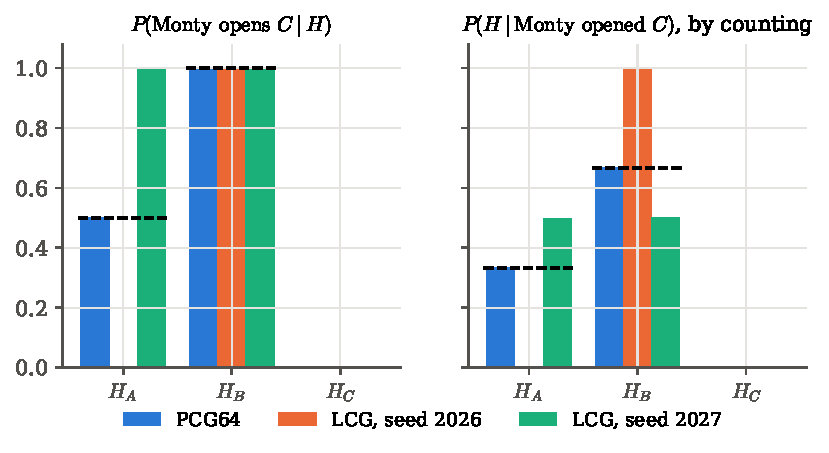
\includegraphics[width=0.95\linewidth]{figures/ch06/monty_generators.pdf}
\caption{Monty Hall simulated with three sources of integers. Left: the measured
probability that Monty opens $C$ under each location of the car. With PCG64
(blue) it is $\tfrac12$, $1$, $0$ (dashed). With the textbook generator the coin
never varies, so under $H_A$ Monty either never (orange) or always (green) opens
$C$. Right: where the car was, among the games in which Monty opened $C$. The
wrong probability under $H_A$ produces the wrong posterior: $0$ and $1$, or
$\tfrac12$ and $\tfrac12$, instead of $\tfrac13$ and $\tfrac23$.}
\label{6a:fig:monty-generators}
\end{figure}

This failure is dangerous because nothing gives it away. First, the fraction of
all games that switching wins is $\SixAMontyGoodSwitch$ with numpy, $\SixAMontyBadOneSwitch$ and
$\SixAMontyBadTwoSwitch$ with the textbook generator: the headline number is
right in all three runs, because it does not involve the coin. The damage is
visible only in the conditional question. Second, nothing crashed and nothing
looked odd; the car's location, taken from the same generator, is perfectly
uniform. The cause, derived in \cref{6a:sec:lcg}, is that the lowest bit of this
generator alternates $0,1,0,1,\dots$, so every second integer, the one used for
the coin, has the same lowest bit.

\subsection{What we ask of a stream of random numbers}

The example shows what a source of random numbers must do. A simulation turns
numbers $u_1,u_2,\dots$ into events, and every probability it reports is a
frequency of those events. So the simulation is correct if the $u_i$ behave, for the purpose at
hand, like \newterm{independent draws from the uniform distribution}
\unpack{every $u_i$ equally likely to fall anywhere in $[0,1)$, and knowing some
of them tells nothing about the others} on $[0,1)$, whose density is
\begin{equation}
  g(u)=\begin{cases}1,&0\le u<1,\\ 0,&\text{otherwise}\end{cases}
  \label{6a:eq:uniform}
\end{equation}
\srcref{Cowan}{(3.1)}.

Every Monte Carlo method assumes such numbers. Monte Carlo integration takes them
for granted: to
estimate $\int_a^b h(x)\,\dd x$ we ``generate $X_1,\dots,X_N\sim\mathrm{Unif}(a,b)$''
and average \mainref{p.~404, (24.2)}. So does the idea of representing a
distribution by a large sample of representative values \srcref{Kruschke}{\S7.1}:
the numbers $x$ built from the $u_i$ are treated as simulated measurements, and
the probability of any region is estimated from how many of them fall in it. The
payoff is greatest in many dimensions, where integrating a joint density over a
complicated region by other methods may not be feasible \srcref{Cowan}{Ch.~3}.
In practice we ask a stream of numbers for five things at once.
\begin{enumerate}[itemsep=1pt]
  \item \emph{Statistical quality:} no test that matters for our application can
        distinguish the numbers from independent uniform draws.
  \item \emph{A long period:} the sequence must not repeat within any
        computation we will ever run.
  \item \emph{Reproducibility:} running the program again gives the same numbers,
        so that a result can be checked and a bug can be found.
  \item \emph{Speed:} a large simulation consumes $10^{9}$ to $10^{12}$ numbers.
  \item \emph{Independent streams:} many simulations running at once each need
        their own numbers, with no hidden relations between them.
\end{enumerate}

The obvious source of randomness is physics. Cowan mentions tossing a coin
\srcref{Cowan}{\S3.1}; real devices time radioactive decays, amplify the thermal
(Johnson) noise of a resistor or the shot noise of a diode, or measure which
output port a single photon takes at a beam splitter, where quantum mechanics
itself guarantees that no hidden variable decides the outcome
\srcref{Lambert}{\S12.7, fn.~3}. The operating system of every computer collects
such \newterm{physical entropy} \unpack{bits whose values nobody, including the
computer itself, could have predicted} from the timing jitter of keystrokes, disk
and network interrupts, and from hardware noise sources on the processor chip.
Physical entropy fails requirements 3 to 5 of the list above. It cannot be
replayed, so no result can be reproduced (requirement 3). It is far too slow to
feed one large simulation, let alone many running at once (requirements 4 and
5). And its raw bits are biased and correlated, so they must be post-processed
before use. We therefore use it for one thing only: to choose a starting
point, the seed. Everything else comes from an algorithm.

\begin{workdef}[pseudorandom number generator]
A \newterm{pseudorandom number generator} (PRNG) is a finite set $S$ of
\newterm{states} \unpack{all the bit patterns its memory can hold}, a
\newterm{transition function} $f:S\to S$, an \newterm{output function} $g$ from
states to numbers, and a \newterm{seed} \unpack{the state $s_0$ we start from,
chosen by us}. It produces
\[
  s_{n+1}=f(s_n),\qquad u_{n}=g(s_{n}),\qquad n=1,2,\dots
\]
The sequence $u_1,u_2,\dots$ is completely determined by $s_0$. It is called
\newterm{pseudorandom} \srcref{Cowan}{\S3.1} because it is accepted as random only
in the operational sense of requirement 1.
\emph{Operational test:} apply statistical tests of the hypothesis ``independent
and uniform'' (\cref{6a:sec:tests}), and above all check that the application gives
the same answer with a second, unrelated generator.
\end{workdef}

\begin{figure}[htbp]
\centering
\begin{tikzpicture}[
  st/.style={draw=formblue,thick,rounded corners=2pt,minimum width=14mm,minimum height=8mm,font=\small},
  outb/.style={draw=black!50,rounded corners=2pt,minimum width=12mm,minimum height=7mm,font=\small},
  ar/.style={->,thick}]
  \node[st,fill=fibreorange!15] (s0) at (0,0) {$s_0$};
  \node[st] (s1) at (2.6,0) {$s_1$};
  \node[st] (s2) at (5.2,0) {$s_2$};
  \node[st] (s3) at (7.8,0) {$s_3$};
  \node[font=\small] (dots) at (9.9,0) {$\cdots$};
  \draw[ar,formblue] (s0) -- node[above,font=\footnotesize] {$f$} (s1);
  \draw[ar,formblue] (s1) -- node[above,font=\footnotesize] {$f$} (s2);
  \draw[ar,formblue] (s2) -- node[above,font=\footnotesize] {$f$} (s3);
  \draw[ar,formblue] (s3) -- (dots);
  \foreach \i/\x in {1/2.6,2/5.2,3/7.8} {
    \node[outb] (u\i) at (\x,-1.7) {$u_\i$};
    \draw[ar,black!60] (s\i) -- (u\i);
    \node[font=\footnotesize,anchor=west] at (\x+0.08,-0.85) {$g$};
  }
  \node[font=\footnotesize,align=center,anchor=north] at (0,-0.6) {seed\\(from entropy)};
  \node[font=\footnotesize,anchor=west,align=left] at (9.2,-1.7) {what the\\ program sees};
  \node[font=\footnotesize,anchor=west,align=left] at (9.2,0.75) {hidden state};
\end{tikzpicture}
\caption{A pseudorandom number generator as a deterministic dynamical system. The
state (top row) is updated by the same transition $f$ at every step; the program
sees only the outputs $g(s_n)$ (bottom row). The seed, the only input from
outside, is the orange box.}
\label{6a:fig:state-machine}
\end{figure}

A generator is thus a discrete dynamical system, like the Poincaré map of a
chaotic pendulum. Its apparent randomness comes from the same place as chaos:
nearby states are sent far apart, so after a few steps the output looks
unrelated to the input \srcref{Lambert}{\S12.7}. Kruschke's summary is exact:
PRNGs ``are not actually random; they are in fact deterministic. But the properties
of the sequences they generate mimic the properties of random processes,'' and
every sampling method relies heavily on how well they do so
\srcref{Kruschke}{p.~74, fn.~4}.

\subsection{A finite machine must repeat}

A generator has finitely many states, so it must eventually come back to a state
it has visited, and from then on it repeats. Here is why. The state space $S$ is
finite: a generator with $b$ bits of state has $\abs{S}=2^b$ states. Take the first
$\abs{S}+1$ states $s_0,s_1,\dots,s_{\abs S}$. There are more of them than there
are distinct states, so two must coincide (the \newterm{pigeonhole principle}
\unpack{$n+1$ letters in $n$ pigeonholes put two letters in one hole}):
$s_i=s_j$ for some $i<j\le\abs{S}$. From there on the sequence repeats:
\begin{align}
  s_{j+k}
  &\eqby{1} f^{k}(s_j)
   \eqby{2} f^{k}(s_i)
   \eqby{3} s_{i+k}\qquad\text{for every }k\ge 0 .
  \label{6a:eq:repeat}
\end{align}
\begin{explain}
  \item $s_{j+k}$ is obtained from $s_j$ by applying $f$ $k$ times; $f^k$ means $f$
        composed $k$ times.
  \item $s_j=s_i$, and a function gives the same output for the same input.
  \item The same statement read from $s_i$.
\end{explain}
So the sequence of states, and with it the sequence of outputs, is
\newterm{eventually periodic}: after a \newterm{tail} of $i$ steps it runs round a
cycle whose length $P$, the \newterm{period}, is at most $j-i\le\abs S$. Can the
tail be avoided? Yes, if $f$ is a bijection \unpack{every state has exactly one
predecessor}:
applying $f^{-1}$ to $s_i=s_j$ gives $s_{i-1}=s_{j-1}$, and $i$ applications give
$s_0=s_{j-i}$, so the seed itself lies on the cycle. Good generators are designed
to be bijections with a single cycle through (almost) all $2^b$ states.

\paragraph{Example: von Neumann's middle-square rule.}
The first proposal for a computer generator (von Neumann, in the 1940s) was to
square a four-digit number and keep the middle four digits of the eight-digit
square. Starting from $2916$,
\begin{align*}
  2916^2&=08\,5030\,56\ \to\ 5030, &
  5030^2&=25\,3009\,00\ \to\ 3009,\\
  3009^2&=09\,0540\,81\ \to\ 0540, &
  0540^2&=00\,2916\,00\ \to\ 2916 ,
\end{align*}
where the square is padded with leading zeros to eight digits. After four steps we
are back at the seed: a period of $4$ out of $10^4$ possible states. This is not
bad luck. Running the rule from all $10^4$ seeds, every sequence repeats a value
within $\SixAMidSqMaxSteps$ steps ($\SixAMidSqMeanSteps$ on average), and
$\SixAMidSqZeroPct\%$ of the seeds end stuck at $0$, since $0^2=0$. The
middle-square map is not a bijection (the squares of $x$ and of numbers close to
$x$ share middle digits), so many states funnel into a few short cycles. So a
``chaotic-looking'' rule is not enough; we need one whose cycles we can prove
something about. Linear generators (\cref{6a:sec:lcg}) are such rules.

\paragraph{Example: what the period does to a Monte Carlo estimate.}
A generator that has gone round its cycle adds no new information, yet the error
bar of a simulation keeps shrinking as if it did. To see this, estimate $\pi$ from
pairs $(u_1,u_2)$ of uniform numbers. The pair falls inside
the quarter disc $u_1^2+u_2^2<1$ with probability $p=\pi/4$ (the area of a
quarter of the unit disc), so $\hat\pi=4\times$(fraction of pairs inside). The
usual standard error of a fraction, $\sqrt{p(1-p)/N}$, gives the error bar
$4\sqrt{\hat p(1-\hat p)/N}$ that a script would report (it is derived with the
error of a Monte Carlo average in \cref{6b:sec:sqrtN}); here $\hat p$ is the
fraction of pairs inside and $N$ the number of pairs. Now take the pairs from the tiny generator
$x\mapsto(1229\,x+1)\bmod 2048$ of Lambert's exercise
\srcref{Lambert}{Problem~12.7}, whose period is $2048$ numbers, i.e.\ $1024$
pairs. \Cref{6a:fig:period-cap} shows what happens. Up to about a thousand pairs
the estimate behaves like any other. After one period, each new pair is one we
have already seen, so the estimate stops improving: with $10^6$ pairs it is
$\SixAPiLcgEst$, off by $\SixAPiLcgErr$. The reported error bar knows nothing of
this and keeps shrinking as $1/\sqrt N$, down to $\SixAPiLcgSe$, so the script
reports an estimate that is wrong by thirty of its own standard errors. With
PCG64 the same $10^6$ pairs give $\SixAPiPcgEst\pm\SixAPiPcgSe$, within two
standard errors of $\pi$, as it should be.

\begin{figure}[htbp]
\centering
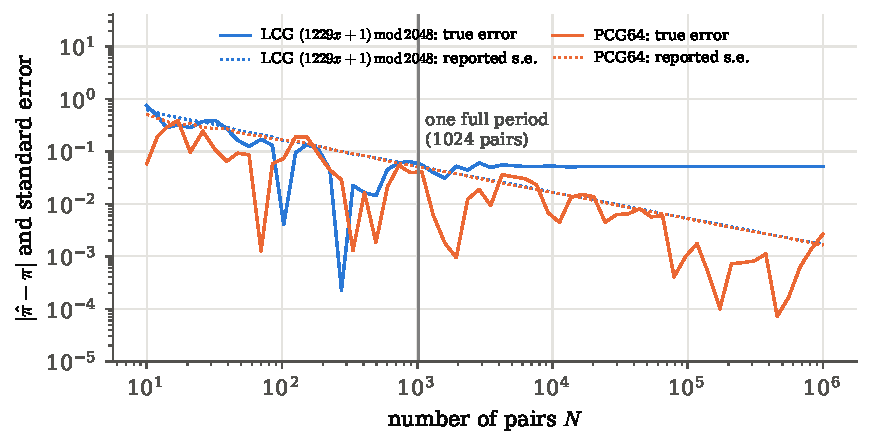
\includegraphics[width=0.85\linewidth]{figures/ch06/period_cap.pdf}
\caption{Estimating $\pi$ from $N$ pairs of uniform numbers. Solid: the actual
error $\abs{\hat\pi-\pi}$; dotted: the standard error the script reports. With
PCG64 (orange) the actual error scatters around the reported one, both falling
as $1/\sqrt N$. With a generator of period $2048$ (blue) the actual error freezes
at $0.05$ once the sequence has gone round its cycle (vertical line), while the
reported error keeps falling.}
\label{6a:fig:period-cap}
\end{figure}

\begin{pitfall}[The error bar cannot see the generator]
A standard error $s/\sqrt N$ is computed under the assumption that the $N$ draws
are independent. If the generator repeats, or if its draws are correlated, the
formula still returns a small number. Nothing in the output of a simulation warns
us; only knowledge of the generator, or a rerun with an unrelated generator, does.
\end{pitfall}

A modern generator never runs out of period: at
$10^9$ numbers per second, PCG64's period of $2^{128}\approx3.4\times10^{38}$
would take $10^{22}$ years. What remains is
requirement 1: making the numbers statistically indistinguishable from
independent uniform draws in every way that could matter, and finding out when
they are not.
\section{Linear congruential generators}
\label{6a:sec:lcg}

The generator that broke Monty's coin in \cref{6a:sec:monty} is a
\emph{linear congruential generator}, the oldest family still in use and, until
the 1990s, the default in most scientific libraries. It deserves a careful look
for two reasons. It is simple enough that we can prove everything about it: its
period, which of its bits are good and which are bad, and where its points lie.
And the generator numpy uses today, PCG64, has a linear congruential generator
inside it. So we ask two questions. With one multiplication and one addition per
step, how long a sequence can we get before it repeats? And which parts of each
number can we trust?

\subsection{The rule and its closed form}

Pick three integers, a \newterm{modulus} $m$, a \newterm{multiplier} $a$ and an
\newterm{increment} $c$, with $0<a<m$ and $0\le c<m$. From a seed $x_0$ in
$\{0,1,\dots,m-1\}$ generate
\begin{equation}
  x_{n+1}=(a\,x_n+c)\bmod m,\qquad u_n=\frac{x_n}{m},
  \label{6a:eq:lcg}
\end{equation}
where $y\bmod m$ \unpack{the remainder of the integer $y$ on division by $m$,
always in $0,\dots,m-1$} keeps the state in range
\srcref{Cowan}{(3.2)--(3.3)}, \srcref{Lambert}{Problem~12.7}. The state is one
integer, the transition is $x\mapsto(ax+c)\bmod m$, and the output divides by $m$.
With $c=0$ the generator is called \newterm{multiplicative}; this is the form Cowan
presents, and there $x_n$ is never $0$ (a zero state would stay zero), so
$u_n=x_n/m$ lies strictly between $0$ and $1$ \srcref{Cowan}{\S3.1}. Implementing
it takes four lines:

\pyfile[firstline=23,lastline=30,firstnumber=23]{code/ch06/lib_prng.py}{A linear congruential generator}

Python integers never overflow, so line 28 is exactly \eqref{6a:eq:lcg}. In C or
Fortran one chooses $m=2^{32}$ or $2^{64}$, and the reduction $\bmod m$ is then free:
it is what the hardware does anyway when an unsigned product overflows.

Where is the state after $n$ steps? Applying the rule $n$ times answers this with
a closed form that we will use repeatedly. For $a\neq1$,
\begin{align}
  x_n
  &\eqby{1} a\,x_{n-1}+c
   \eqby{2} a^2x_{n-2}+ac+c
   \eqby{3} a^n x_0+c\,(a^{n-1}+\dots+a+1)\nonumber\\
  &\eqby{4} a^n x_0+c\,\frac{a^n-1}{a-1}\pmod m .
  \label{6a:eq:closed}
\end{align}
\begin{explain}
  \item The rule \eqref{6a:eq:lcg}; the notation ``$\pmod m$'' at the end means
        every equality in the chain holds up to multiples of $m$. Reducing after
        each step or once at the end gives the same remainder, because
        remainders of sums and products depend only on the remainders of the
        terms.
  \item Substitute the rule for $x_{n-1}$.
  \item Repeat $n$ times; each step multiplies what is there by $a$ and adds $c$.
  \item Geometric sum. The fraction $(a^n-1)/(a-1)$ is an integer (it equals the
        sum on the previous line), so this is an integer identity before we reduce.
\end{explain}
In particular, for a multiplicative generator $x_n=a^nx_0\bmod m$: the whole
sequence is powers of $a$.

\paragraph{Example: Lambert's toy generator.}
Take $a=2$, $c=3$, $m=10$ and the seed $x_0=5$ \srcref{Lambert}{Problem~12.7.2}:
\[
  5\ \to\ (2\cdot5+3)\bmod10=3\ \to\ 9\ \to\ (21\bmod 10)=1\ \to\ 5\ \to\ 3\ \to\cdots
\]
The sequence comes back to the seed after $4$ steps, although there are $10$
states: the period is $4$. \Cref{6a:fig:functional-graph}
shows the transition of every state. The seed $7$ is a fixed point
($2\cdot7+3=17\to7$), and the seeds $0,2,4,6,8$ each lead into the cycle or the
fixed point after one step, so they have a tail. The rule is not a bijection:
$3$ has two predecessors, $0$ and $5$, because $2x$ and $2(x+5)$ differ by $10$.
Whenever $a$ shares a factor with $m$, two states that differ by $m/\gcd(a,m)$ are
sent to the same place, and the tails of \cref{6a:eq:repeat} appear.

\begin{figure}[htbp]
\centering
\begin{tikzpicture}[
  stn/.style={circle,draw=formblue,thick,minimum size=7mm,inner sep=0pt,font=\small},
  tln/.style={circle,draw=black!40,minimum size=7mm,inner sep=0pt,font=\small},
  ar/.style={->,thick,formblue},
  ta/.style={->,thick,black!45}]
  \node[stn] (5) at (0,1.3) {5};
  \node[stn] (3) at (1.3,0) {3};
  \node[stn] (9) at (0,-1.3) {9};
  \node[stn] (1) at (-1.3,0) {1};
  \draw[ar] (5) to[bend left=25] (3);
  \draw[ar] (3) to[bend left=25] (9);
  \draw[ar] (9) to[bend left=25] (1);
  \draw[ar] (1) to[bend left=25] (5);
  \node[tln] (0) at (3.0,0.9) {0};
  \node[tln] (8) at (0,-2.9) {8};
  \node[tln] (4) at (-3.0,0) {4};
  \node[tln] (6) at (0,2.9) {6};
  \draw[ta] (0) -- (3);
  \draw[ta] (8) -- (9);
  \draw[ta] (4) -- (1);
  \draw[ta] (6) -- (5);
  \node[stn,draw=bdryred] (7) at (5.2,0) {7};
  \node[tln] (2) at (5.2,1.6) {2};
  \draw[ta] (2) -- (7);
  \draw[->,thick,bdryred] (7.south east) arc[start angle=120,end angle=-150,radius=3.2mm];
\end{tikzpicture}
\caption{Every state of $x\mapsto(2x+3)\bmod 10$ and where it goes. The seeds $1$,
$3$, $5$, $9$ lie on a cycle of length $4$ (blue); the seed $7$ is a fixed point
(red); the even seeds are not on any cycle and fall into one after a single step
(grey). Because $2$ and $10$ share the factor $2$, two states always share each
image.}
\label{6a:fig:functional-graph}
\end{figure}

\subsection{How long can the period be?}

\paragraph{Multiplicative generators with a prime modulus.}
Let $c=0$ and $m$ prime, and start from any $x_0\neq0$. When does the sequence
come back to its seed? By \eqref{6a:eq:closed} $x_n=a^nx_0\bmod m$, so it returns
exactly when
\begin{align}
  x_n=x_0
  &\quad\relby{1}{\iff}\quad a^nx_0\equiv x_0\pmod m
   \quad\relby{2}{\iff}\quad (a^n-1)\,x_0\equiv0\pmod m\nonumber\\
  &\quad\relby{3}{\iff}\quad a^n\equiv1\pmod m .
  \label{6a:eq:order}
\end{align}
\begin{explain}
  \item The closed form \eqref{6a:eq:closed} with $c=0$; ``$\equiv\ (\bmod m)$''
        means ``differs by a multiple of $m$''.
  \item Move $x_0$ to the left and factor.
  \item $m$ is prime and does not divide $x_0$ (because $0<x_0<m$), so it must
        divide $a^n-1$. A prime that divides a product divides one of the factors.
\end{explain}
The period is therefore the smallest $n\ge1$ with $a^n\equiv1\pmod m$, the
\newterm{order} of $a$ modulo $m$, and it is the same for every seed. How large
can it be? Fermat's little theorem says $a^{m-1}\equiv1\pmod m$ for prime $m$. Call
the order $P$ and write $m-1=qP+r$ with $0\le r<P$. Then
$a^r=a^{m-1}(a^P)^{-q}\equiv1$, and since $P$ is the smallest positive power that
gives $1$, $r$ must be $0$. So the order divides $m-1$, and the period is at most
$m-1$ (all states except $0$). It equals $m-1$ exactly when $a$ is a
\newterm{primitive root} \unpack{its powers $a,a^2,\dots,a^{m-1}$ run through
all nonzero remainders}.

\paragraph{Example: the two multipliers modulo 7.}
With $m=7$ and $a=3$, starting from $1$:
$1\to3\to9\bmod7=2\to6\to18\bmod7=4\to12\bmod7=5\to15\bmod7=1$. The period is
$6=m-1$; $3$ is a primitive root. With $a=2$: $1\to2\to4\to8\bmod7=1$, period $3$,
because $2^3=8\equiv1$. From the seed $3$ the same multiplier gives $3\to6\to5\to3$,
a different cycle of the same length: the six nonzero states split into two
cycles of three.

Cowan's example generator is of this kind: $m=2147483399$ is prime and
$a=40692$ has period $m-1\approx2\times10^9$ \srcref{Cowan}{\S3.1},
\cite{LEcuyer1988}. In the 1980s that was respectable. Today a single core produces
$10^9$ numbers per second, so the whole period is used up in about
\begin{equation*}
  \frac{2.1\times10^{9}\ \text{numbers}}{10^{9}\ \text{numbers/s}}\approx 2\ \text{s},
\end{equation*}
and a simulation that runs for an hour would go round the cycle about
seventeen hundred times. L'Ecuyer's remedy in the same paper was to combine two such
generators with different prime moduli, so that the period becomes of the order of
the product of the two periods (about $2\times10^{18}$); this idea of a small cheap transition with a very large period runs
through all modern designs. Cowan's example of a much longer period is the RANMAR
generator, about $10^{43}$ \srcref{Cowan}{\S3.1}.

\paragraph{Full period with an increment.}
With $c\neq0$ the state $0$ is allowed, so all $m$ states could in principle
form one cycle. Which choices of $a$, $c$ and $m$ achieve this? A classical theorem
gives the exact answer.

\begin{keyidea}[Full period of $x\mapsto(ax+c)\bmod m$ (Hull and Dobell)]
The generator has period $m$ for every seed if and only if
\begin{enumerate}[itemsep=0pt]
  \item $c$ and $m$ have no common factor, $\gcd(c,m)=1$;
  \item $a-1$ is divisible by every prime that divides $m$;
  \item $a-1$ is divisible by $4$ if $m$ is divisible by $4$.
\end{enumerate}
\end{keyidea}

Why the first condition is needed can be seen in three lines. Suppose
$d=\gcd(c,m)>1$ and start from $x_0=0$. By \eqref{6a:eq:closed}, $x_n=c\,(a^{n-1}+\dots+1)\bmod m$. Every term
is a multiple of $d$, and reducing modulo $m$ (itself a multiple of $d$) keeps it
a multiple of $d$. So only the $m/d$ multiples of $d$ are ever visited, and the
period is at most $m/d<m$. The second and third conditions force $a\equiv1$ modulo every prime that
divides $m$ (and modulo $4$ when $4$ divides $m$). The map then behaves enough
like $x\mapsto x+c$, which steps through every remainder in turn, that it too
visits every state before returning. Their proof is elementary number theory, and
nothing later depends on it.

\paragraph{Example: a full cycle of sixteen.}
For $m=16=2^4$ take $a=5$, $c=3$. Then $\gcd(3,16)=1$, and $a-1=4$ is divisible by
$2$ (the only prime in $16$) and by $4$. From $x_0=0$ the sequence is
\[
  3,\ 2,\ 13,\ 4,\ 7,\ 6,\ 1,\ 8,\ 11,\ 10,\ 5,\ 12,\ 15,\ 14,\ 9,\ 0,
\]
all sixteen states once each. Lambert's generator
$x\mapsto(1229x+1)\bmod2048$ with $2048=2^{11}$, also satisfies the conditions
($c=1$; $1228=4\cdot307$), and indeed its period is $\SixALamAPeriod$. So does his
second, $x\mapsto(1597x+51749)\bmod244944$ \srcref{Lambert}{Problem~12.7.6}: here
$244944=2^4\cdot3^7\cdot7$, $51749$ is divisible by none of $2,3,7$, and
$1596=2^2\cdot3\cdot7\cdot19$ is divisible by $2$, $3$, $7$ and $4$, and the
period comes out as $\SixALamBPeriod$. Lambert's question ``what is the maximum
period?'' \srcref{Lambert}{Problem~12.7.1} has the answer $m$, reached exactly
under these three conditions.

\subsection{The low bits of a power-of-two modulus}

Look again at the sixteen numbers above and write down only whether each is odd or
even: $1,0,1,0,\dots$. The lowest bit alternates. This is not an accident of the
example. Suppose $m=2^k$ and look at the lowest $j$ bits of the state, i.e.\ at
$x_n\bmod2^j$ with $j\le k$. Then
\begin{align}
  x_{n+1}\bmod 2^j
  &\eqby{1}\bigl((a x_n+c)\bmod 2^k\bigr)\bmod 2^j
   \eqby{2}(a x_n+c)\bmod 2^j
   \eqby{3}\bigl(a\,(x_n\bmod2^j)+c\bigr)\bmod 2^j .
  \label{6a:eq:lowbits}
\end{align}
\begin{explain}
  \item The rule \eqref{6a:eq:lcg} with $m=2^k$, then reduction modulo $2^j$.
  \item $2^j$ divides $2^k$, so removing multiples of $2^k$ does not change the
        remainder modulo $2^j$.
  \item Replacing $x_n$ by its remainder changes $ax_n$ by a multiple of $2^j$.
\end{explain}
The lowest $j$ bits therefore form an LCG of their own, with modulus $2^j$ and no
input from the higher bits. It has only $2^j$ states, so its period is at most
$2^j$: the lowest bit has period at most $2$, the lowest two bits at most $4$,
and so on. For $j=1$, $a$ odd and $c$ odd (as the full-period conditions require),
$x_{n+1}\equiv x_n+1\pmod 2$: the parity flips at every step.

\paragraph{Example: the bits of a 32-bit generator.}
\Cref{6a:fig:lowbits} shows the $32$ bits of the first $64$ outputs of
$x\mapsto(1664525x+1013904223)\bmod2^{32}$, the generator of the Monty example.
The measured periods of bits $0,1,2,3$ are $\SixABitPerZero$, $\SixABitPerOne$,
$\SixABitPerTwo$, $\SixABitPerThree$, and bit $11$ has period $\SixABitPerEleven$:
bit $j$ has period exactly $2^{j+1}$. The Monty simulation of
\cref{6a:sec:monty} drew two integers per game and took the coin from the second,
$x\bmod2$, which is bit $0$ of every second output. Since bit $0$ alternates,
every second output has the same parity, and the coin never changes. The cure is
never to use the low bits of such a generator. Take the \emph{high} bits instead, e.g.\
$\lfloor 2u_n\rfloor$ with $u_n=x_n/2^{32}$, whose period is the full $2^{32}$.

\begin{figure}[htbp]
\centering
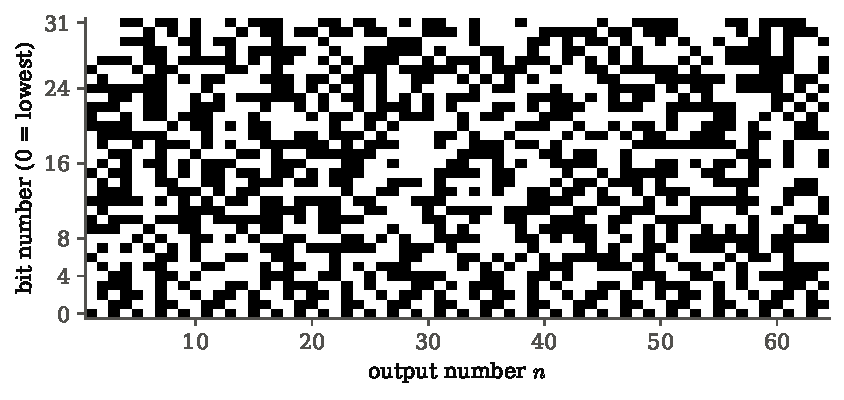
\includegraphics[width=0.85\linewidth]{figures/ch06/lcg_lowbits.pdf}
\caption{The bits of the first 64 outputs of the 32-bit linear congruential
generator used in the Monty example (black $=1$). The lowest rows are periodic
with periods $2$, $4$, $8$, \dots; only the upper rows look random. The lowest row
alternates, which is why taking $x\bmod2$ from every second output gave Monty a
coin that never changes.}
\label{6a:fig:lowbits}
\end{figure}

\begin{pitfall}[The remainder trick]
Writing \texttt{x \% n} to get an integer in $0,\dots,n-1$ uses the \emph{lowest}
bits of $x$. For a power-of-two linear congruential generator those are the worst
bits it has. It also has a bias whenever $n$ does not divide the number of
possible values of $x$. Library functions such as \texttt{rng.integers(n)} avoid
both problems.
\end{pitfall}

A full period says nothing about how the numbers are arranged within it. The
tiny generator $x\mapsto(1229x+1)\bmod2048$ visits every one of its $2048$ states,
yet the left panel of \cref{6a:fig:lcg-pairs}, which plots each output against the
next, shows that consecutive pairs lie on six parallel lines (one of them very short)
\srcref{Lambert}{Problem~12.7.5}. Lambert's larger generator and RANDU look fine
in the same plot. The lines come from a lattice that every linear congruential
generator carries (\cref{6a:sec:lattice}); for RANDU that lattice shows up in
three dimensions.

\begin{figure}[htbp]
\centering
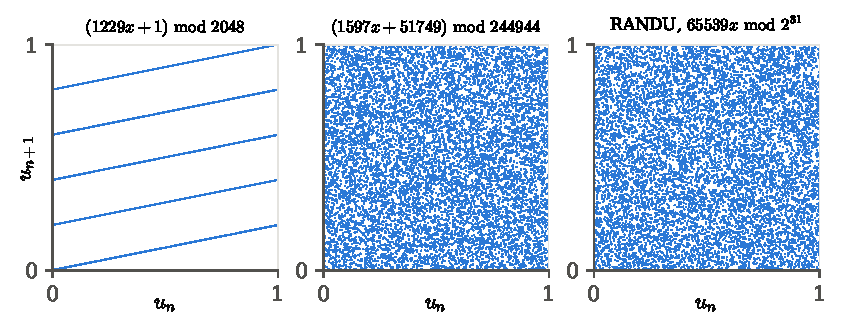
\includegraphics[width=\linewidth]{figures/ch06/lcg_pairs.pdf}
\caption{Consecutive pairs $(u_n,u_{n+1})$ from three linear congruential
generators. Left: all 2048 pairs of $x\mapsto(1229x+1)\bmod2048$ lie on a few
parallel lines. Middle and right: $10^4$ pairs from Lambert's second generator and
from RANDU, which show no structure at this resolution.}
\label{6a:fig:lcg-pairs}
\end{figure}
\section{Random numbers fall mainly in the planes}
\label{6a:sec:lattice}

Many simulations use the uniform numbers in groups. A point in a detector volume
needs three coordinates; a photon's direction needs two angles and its energy a
third number; a rejection-sampling step (taken up later in the chapter) needs a
candidate and a test value. Group consecutive outputs of a linear congruential
generator into $t$-tuples $(u_n,u_{n+1},\dots,u_{n+t-1})$ and plot them as points
in the unit cube $[0,1)^t$. For independent uniform numbers the points would fill
the cube evenly. In 1968 Marsaglia showed that for \emph{every} multiplicative
linear congruential generator they do something else: they lie on a family of
parallel hyperplanes, and for some generators on very few of them
\cite{Marsaglia1968}. The six lines in the left panel of \cref{6a:fig:lcg-pairs}
were the two-dimensional case. So three questions follow. Where exactly do the
$t$-tuples lie? How many planes are there? And how do we measure how bad that is?

\subsection{Why the points form a lattice}

The points are far from independent because a whole $t$-tuple is fixed by one
number, the state at its start. Take a multiplicative generator,
$x_{n+1}=ax_n\bmod m$ (\cref{6a:eq:lcg} with $c=0$), and its outputs $u_n=x_n/m$.
By the closed form \eqref{6a:eq:closed},
$x_{n+j}=a^jx_n\bmod m$, i.e.\ $a^jx_n$ minus some integer multiple $k_jm$ of $m$.
Dividing by $m$, the $t$-tuple that starts at $x_n$ is
\begin{align}
  \bm u
  &\equiv(u_n,u_{n+1},\dots,u_{n+t-1})
   \eqby{1}\frac{x_n}{m}\,(1,a,a^2,\dots,a^{t-1})-(0,k_1,k_2,\dots,k_{t-1}) .
  \label{6a:eq:lattice}
\end{align}
\begin{explain}
  \item $u_{n+j}=x_{n+j}/m=(a^jx_n-k_jm)/m=a^jx_n/m-k_j$ for $j=1,\dots,t-1$,
        and $u_n=x_n/m$.
\end{explain}
Every tuple is therefore an integer multiple of the single vector
$\bm v=(1,a,\dots,a^{t-1})/m$ plus a vector of integers. The set of all such
combinations $\{x\,\bm v+\bm z:\ x\in\Z,\ \bm z\in\Z^t\}$ is a
\newterm{lattice} \unpack{a regular, crystal-like grid of points: all integer
combinations of a few fixed vectors}. The generator's tuples are the points of
this lattice that fall in the unit cube (at most $m-1$ of them, one for each
state). In crystal language: the points of a generator are the atoms of a crystal,
and a crystal is organised in lattice planes.

Where do the planes come from? A family of parallel planes is described by a
normal vector $\bm h$: the planes are $\bm h\cdot\bm u=k$ for $k=0,\pm1,\pm2,\dots$.
So we ask which integer vectors $\bm h=(h_1,\dots,h_t)$ make $\bm h\cdot\bm u$ an
integer for every tuple. The answer is every $\bm h$ with
\begin{equation}
  h_1+a\,h_2+a^2h_3+\dots+a^{t-1}h_t\equiv0\pmod m .
  \label{6a:eq:dual}
\end{equation}
To check it, compute $\bm h\cdot\bm u$ for any tuple:
\begin{align}
  \bm h\cdot\bm u
  &\eqby{1}\frac{x_n}{m}\,\bigl(h_1+ah_2+\dots+a^{t-1}h_t\bigr)-\sum_{j\ge1}h_{j+1}k_j
   \eqby{2}x_n\,q-\sum_{j\ge1}h_{j+1}k_j\ \in\ \Z ,
  \label{6a:eq:planes}
\end{align}
\begin{explain}
  \item Dot $\bm h$ into \eqref{6a:eq:lattice}.
  \item By \eqref{6a:eq:dual} the bracket is $q\,m$ for some integer $q$; what is
        left is a sum of products of integers.
\end{explain}
so every tuple lies on one of the parallel hyperplanes $\bm h\cdot\bm u=k$,
$k\in\Z$. The integer vectors that satisfy \eqref{6a:eq:dual} form a lattice of
their own, the \newterm{dual lattice} \unpack{the integer vectors $\bm h$ with
$\bm h\cdot\bm u$ an integer for every point of the generator}, and each nonzero
$\bm h$ in it defines one family of planes. Two facts about such a family follow
from elementary geometry.
\begin{itemize}[itemsep=1pt]
  \item \emph{Spacing.} The planes $\bm h\cdot\bm u=k$ and $\bm h\cdot\bm u=k+1$ are
        a distance $1/\abs{\bm h}$ apart, with $\abs{\bm h}=\sqrt{h_1^2+\dots+h_t^2}$.
        (A plane $\bm h\cdot\bm u=k$ lies at distance $k/\abs{\bm h}$ from the
        origin, along the unit normal $\bm h/\abs{\bm h}$.)
  \item \emph{Number.} Inside the unit cube, $\bm h\cdot\bm u$ lies strictly between
        $\sum_{h_i<0}h_i$ and $\sum_{h_i>0}h_i$, an open interval of length
        $\abs{h_1}+\dots+\abs{h_t}$. It therefore contains at most
        $\abs{h_1}+\dots+\abs{h_t}$ integers, and the points lie on at most that
        many planes. (When the endpoints are integers that the points never
        reach, as for a multiplicative generator, the interval contains one
        fewer, $\abs{h_1}+\dots+\abs{h_t}-1$.)
\end{itemize}
So a \emph{short} dual vector is bad news: it means few planes, far apart, with
nothing in between. For an increment $c\neq0$ the tuples are the same lattice shifted by a
constant vector, so the planes are the same, merely displaced.

\begin{figure}[htbp]
\centering
\begin{tikzpicture}[scale=5.2]
  \draw[black!50] (0,0) rectangle (1,1);
  \begin{scope}
    \clip (0,0) rectangle (1,1);
    \foreach \k in {0,1,2} {
      \draw[formblue!55,thick] ({\k/3},0) -- ({(\k+1)/3},1);
    }
  \end{scope}
  \foreach \x in {1,...,30} {
    \pgfmathtruncatemacro{\y}{mod(3*\x,31)}
    \fill[fibreorange!85!black] ({\x/31},{\y/31}) circle (0.26pt);
  }
  \draw[->,thick,tangentgreen] (0.5,0.5) -- (0.8,0.4);
  \node[tangentgreen!70!black,font=\footnotesize,anchor=north] at (0.66,0.38) {$\bm h/\abs{\bm h}^2$};
  \node[font=\footnotesize,anchor=north] at (0.5,-0.02) {$u_n$};
  \node[font=\footnotesize,anchor=east] at (-0.02,0.5) {$u_{n+1}$};
  \node[font=\footnotesize,anchor=north] at (0,-0.02) {$0$};
  \node[font=\footnotesize,anchor=north] at (1,-0.02) {$1$};
  \node[font=\footnotesize,anchor=east] at (-0.02,1) {$1$};
  \node[font=\footnotesize,formblue,anchor=west] at (1.02,0.95) {$3u_n-u_{n+1}=0$};
  \node[font=\footnotesize,formblue,anchor=west] at (1.02,0.55) {$3u_n-u_{n+1}=1$};
  \node[font=\footnotesize,formblue,anchor=west] at (1.02,0.15) {$3u_n-u_{n+1}=2$};
\end{tikzpicture}
\caption{All 30 pairs $(u_n,u_{n+1})$ of the toy generator $x\mapsto3x\bmod31$
(orange dots). The dual vector $\bm h=(3,-1)$ satisfies $3-3\cdot1\equiv0$, so
every pair has $3u_n-u_{n+1}$ equal to $0$, $1$ or $2$ and lies on one of three
parallel lines (blue). The green arrow joins two neighbouring lines along their
common normal; its length is the gap $1/\abs{\bm h}=1/\sqrt{10}$.}
\label{6a:fig:dual-lattice}
\end{figure}

\paragraph{Example: the toy generator modulo 31.}
For $x\mapsto3x\bmod31$ in two dimensions, condition \eqref{6a:eq:dual} reads
$h_1+3h_2\equiv0\pmod{31}$. The vector $\bm h=(3,-1)$ satisfies it
($3-3=0$), so every pair has $3u_n-u_{n+1}\in\Z$. Inside the square
$3u_n-u_{n+1}$ lies between $-1$ and $3$, so it is $0$, $1$ or $2$ (the value $-1$
would need $u_{n+1}=1$ and $u_n=0$, which cannot occur): three lines, a distance
$1/\sqrt{3^2+1^2}=0.32$ apart (\cref{6a:fig:dual-lattice}). No shorter dual vector
exists: the only other candidates with $\abs{\bm h}\le\sqrt{10}$ are
$(\pm1,0)$, $(0,\pm1)$, $(\pm1,\pm1)$, $(\pm2,\pm1)$, $(\pm1,\pm2)$ and so on, and
none gives $h_1+3h_2$ divisible by $31$.

\paragraph{Example: Lambert's generator.}
For $x\mapsto(1229x+1)\bmod2048$ the vector $\bm h=(1,-5)$ works:
$1-5\cdot1229=-6144=-3\cdot2048$. So $u_n-5u_{n+1}$ takes only integer values
(shifted by the constant $-5/2048$ that the increment contributes), at most
$\abs{1}+\abs{-5}=6$ of them, and the pairs lie on six lines a distance
$1/\sqrt{26}=0.20$ apart. That is the left panel of \cref{6a:fig:lcg-pairs}. A good
generator with $2048$ states could have spread its pairs over lines a few
hundredths apart.

\subsection{RANDU's fifteen planes}

RANDU was the generator supplied with IBM's System/360 scientific library in the
1960s, and it was copied into many other systems. It is multiplicative, with
\[
  x_{n+1}=65539\,x_n\bmod 2^{31},\qquad 65539=2^{16}+3 ,
\]
seeded with an odd $x_0$. The multiplier was chosen because multiplying by
$2^{16}+3$ is a shift and two additions, fast on the hardware of the time. That
choice is its downfall. To see why, ask how three consecutive outputs are related.
Two steps multiply the state by $a^2$, $x_{n+2}=a^2x_n\bmod2^{31}$, so we need
$a^2$ modulo $2^{31}$:
\begin{align}
  a^2
  &\eqby{1}(2^{16}+3)^2
   \eqby{2}2^{32}+6\cdot2^{16}+9
   \eqby{3}6\cdot2^{16}+9\pmod{2^{31}}\nonumber\\
  &\eqby{4}6\,(2^{16}+3)-18+9
   \eqby{5}6a-9 \pmod{2^{31}} .
  \label{6a:eq:randu}
\end{align}
\begin{explain}
  \item $a=65539=2^{16}+3$.
  \item $(p+q)^2=p^2+2pq+q^2$ with $p=2^{16}$, $q=3$.
  \item $2^{32}=2\cdot2^{31}$ is a multiple of the modulus.
  \item Write $6\cdot2^{16}=6\,(2^{16}+3)-18$.
  \item Collect: $-18+9=-9$, and $2^{16}+3=a$.
\end{explain}
So $a^2$ is a small combination of $a$ and $1$. Multiplying \eqref{6a:eq:randu}
by $x_n$ gives $x_{n+2}=a^2x_n\equiv6ax_n-9x_n
\equiv6x_{n+1}-9x_n$, that is, every output is fixed by the two before it:
\begin{equation}
  x_{n+2}-6x_{n+1}+9x_n\equiv0\pmod{2^{31}}
  \qquad\Longrightarrow\qquad
  9u_n-6u_{n+1}+u_{n+2}\in\Z .
  \label{6a:eq:randu-planes}
\end{equation}
This is \eqref{6a:eq:planes} with the dual vector $\bm h=(9,-6,1)$. Inside the cube
$9u_n-6u_{n+1}+u_{n+2}$ lies strictly between $-6$ and $10$, so it is one of the
fifteen integers $-5,-4,\dots,9$. \emph{All} triples of RANDU lie on fifteen
parallel planes, a distance $1/\sqrt{81+36+1}=1/\sqrt{118}\approx\SixASpecRanduThreeD$
apart. A small ball of diameter just under $0.09$ can sit between two neighbouring
planes and contain no point at all. Knuth's verdict, quoted ever since, was that the very name RANDU is enough to
bring dismay into the eyes and stomachs of many computer scientists.

The script \pyname{04_randu_planes.py} generates $30000$ consecutive triples from
the seed $1$, computes $9u_n-6u_{n+1}+u_{n+2}$ for each, and checks that it is an
exact integer; it takes exactly $\SixARanduNplanes$ values, from $\SixARanduKmin$
to $\SixARanduKmax$. The planes are invisible from a generic viewpoint, but
looking along them (viewing direction $(1,1.5,0)$, which is perpendicular to the
normal $(9,-6,1)$) they appear edge-on as fifteen lines
(\cref{6a:fig:randu}). This is Marsaglia's classic picture \cite{Marsaglia1968}.

\begin{figure}[htbp]
\centering
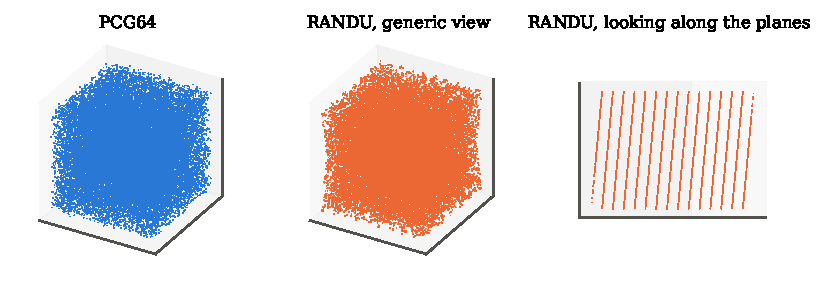
\includegraphics[width=\linewidth]{figures/ch06/randu_planes.pdf}
\caption{Thirty thousand consecutive triples $(u_n,u_{n+1},u_{n+2})$ in the unit
cube. Left: from PCG64. Middle: from RANDU, seen from the same generic angle;
nothing looks wrong. Right: RANDU seen along the direction $(1,1.5,0)$, which lies
in its planes $9u_n-6u_{n+1}+u_{n+2}=k$; the planes appear edge-on, fifteen of
them.}
\label{6a:fig:randu}
\end{figure}

What does this do to a physics simulation? Anything that uses three consecutive
numbers as a point in space samples only fifteen slices of the space. A detector
acceptance computed by throwing points into a cube, a random walk in three
dimensions, or a three-body phase-space generator would all be biased, and the
bias does not shrink with $N$: it is a property of the generator, not a
statistical fluctuation.

\subsection{The spectral test}

How do we measure how bad a generator's lattice is in $t$ dimensions? By the
widest gap between its planes, because a wide gap is a slab of the cube that no
tuple ever visits. The gap of a family is $1/\abs{\bm h}$, so the widest gap
belongs to the shortest nonzero dual vector. Its length
\begin{equation}
  \nu_t=\min\bigl\{\abs{\bm h}:\ \bm h\in\Z^t,\ \bm h\neq\bm0,\
  h_1+ah_2+\dots+a^{t-1}h_t\equiv0\pmod m\bigr\},
  \qquad d_t=\frac1{\nu_t},
  \label{6a:eq:spectral}
\end{equation}
gives the largest distance $d_t$ between adjacent hyperplanes that hold all the
$t$-tuples. Computing $\nu_t$ for $t=2,\dots,6$ or $8$ is the \newterm{spectral
test} (the name comes from its origin in Fourier analysis: $\bm h$ is a wave vector
in which the empirical density of the points has a spike, the lattice Bragg
peak of the crystal). A small $d_t$ means that even the most widely spaced family of planes is dense,
so the points come close to filling the cube.

\begin{workdef}[spectral test]
For a linear congruential generator with multiplier $a$ and modulus $m$, and a
dimension $t$: find the shortest nonzero integer vector $\bm h$ with
$h_1+ah_2+\dots+a^{t-1}h_t\equiv0\pmod m$. Its length is $\nu_t$; the
$t$-tuples lie on hyperplanes $\bm h\cdot\bm u\in\Z$ a distance $d_t=1/\nu_t$
apart. \emph{Operational test:} compare $d_t$ with the smallest gap any lattice with
$m$ points per unit volume could have (\cref{6a:eq:ideal}); a generator whose
$d_t$ is many times larger fails.
\end{workdef}

Finding the shortest vector of a lattice is a classic problem, and in low
dimension it is easy: the script \pyname{05_spectral_test.py} writes down a basis of the dual
lattice, namely $(m,0,\dots,0)$ and $(-a^{j-1}\bmod m)\,\bm e_1+\bm e_j$ for
$j=2,\dots,t$ (any solution of \eqref{6a:eq:dual} is an integer combination of
these), reduces it with the Lenstra--Lenstra--Lov\'asz (LLL) algorithm
\unpack{repeated Gram--Schmidt-like steps that make the basis vectors short and
nearly orthogonal}, and then searches small integer combinations of the reduced
vectors for the shortest one. For RANDU in $t=3$ it finds $\bm h=(9,-6,1)$ with
$\nu_3=\SixASpecRanduThreeNu$, confirming \eqref{6a:eq:randu-planes}. The same
calculation for three classic generators is plotted in \cref{6a:fig:spectral}.

\begin{figure}[htbp]
\centering
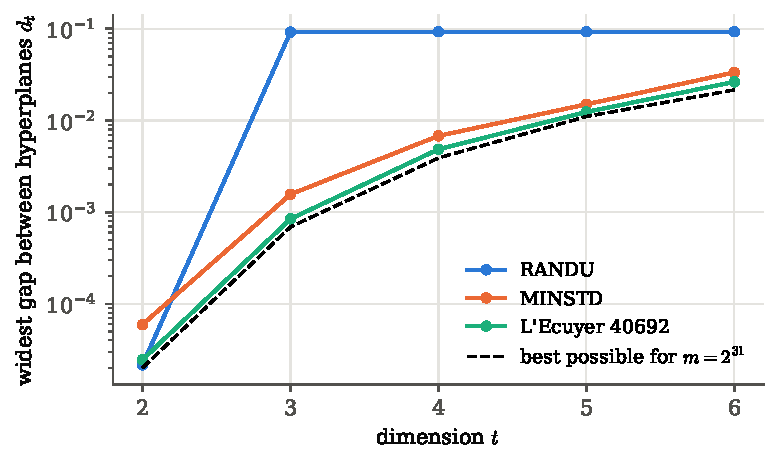
\includegraphics[width=0.75\linewidth]{figures/ch06/spectral.pdf}
\caption{The spectral test for three multiplicative generators with $m\approx2^{31}$:
the widest gap $d_t$ between the hyperplanes that hold the $t$-tuples. The
dashed line is the smallest gap any lattice with $2^{31}$ points per unit volume
can have. RANDU is near-ideal in two dimensions and then jumps to
$d_3\approx0.09$, where it stays. MINSTD ($a=16807$, $m=2^{31}-1$) and
L'Ecuyer's $a=40692$ stay within a factor of about three of the ideal.}
\label{6a:fig:spectral}
\end{figure}

\paragraph{How small can the gap be?}
Even the best multiplier leaves gaps of a certain size, and Minkowski's theorem
tells us how large. A lattice with one point per state has $m$ points per unit
volume: the volume of
its unit cell is $1/m$, and its dual lattice has unit-cell volume $m$
(the reciprocal lattice of a crystal has the inverse cell volume, the same fact
from solid-state physics). A lattice cannot have arbitrarily long shortest
vectors at fixed cell volume. \newterm{Minkowski's theorem} \unpack{a convex region,
symmetric about the origin, with volume larger than $2^t$ times the cell volume
must contain a nonzero lattice point} makes this precise. Apply it to the
\newterm{cross-polytope} $\{\bm h:\ \abs{h_1}+\dots+\abs{h_t}\le r\}$, the
$t$-dimensional octahedron:
\begin{align}
  \mathrm{vol}\{\abs{h_1}+\dots+\abs{h_t}\le r\}
  &\eqby{1}2^t\,\frac{r^t}{t!}
   \ \relby{2}{\ge}\ 2^t\,m
   \quad\iff\quad r\ \ge\ (t!\,m)^{1/t} .
  \label{6a:eq:minkowski}
\end{align}
\begin{explain}
  \item The octahedron is $2^t$ copies (one per sign pattern) of the simplex
        $\{h_i\ge0,\ \sum h_i\le r\}$, whose volume is $r^t/t!$ (for $t=2$, a
        triangle of area $r^2/2$; for $t=3$, a tetrahedron of volume $r^3/6$).
  \item Minkowski's condition, with the dual cell volume $m$.
\end{explain}
So for $r=(t!\,m)^{1/t}$ the octahedron contains a nonzero dual vector $\bm h$
with $\abs{h_1}+\dots+\abs{h_t}\le r$, and by the ``number'' bullet above, the
$t$-tuples lie on at most $(t!\,m)^{1/t}$ hyperplanes. This is Marsaglia's theorem
\cite{Marsaglia1968}: \emph{every} multiplicative generator with modulus $m$ puts
its $t$-tuples on at most $(t!\,m)^{1/t}$ parallel hyperplanes. For $m=2^{32}$ the
bound is $\SixAMarsBoundThree$ planes in three dimensions and only
$\SixAMarsBoundTen$ in ten. No choice of multiplier can avoid it; a good choice
only avoids being much worse. The sharpest statement of the same kind uses the
Hermite constants $\gamma_t$ of lattice theory \unpack{the largest possible value of
(shortest vector)$^2$/(cell volume)$^{2/t}$ over all lattices in $t$ dimensions}
and gives the smallest possible gap,
\begin{equation}
  d_t\ \ge\ \frac{1}{\gamma_t^{1/2}\,m^{1/t}},\qquad
  \gamma_2=\bigl(\tfrac43\bigr)^{1/2},\ \gamma_3=2^{1/3},\ \gamma_4=2^{1/2},\ \dots,
  \label{6a:eq:ideal}
\end{equation}
the dashed line in \cref{6a:fig:spectral}: for $m=2^{31}$ and $t=3$ it is
$\SixASpecRanduThreeIdeal$, a hundred times smaller than RANDU's gap.

\paragraph{Example: two generators that pass.}
MINSTD, $x\mapsto16807\,x\bmod(2^{31}-1)$, the ``minimal standard'' of the 1990s,
has $d_2=\SixASpecMinstdTwoD$ and $d_3=\SixASpecMinstdThreeD$, and L'Ecuyer's
$a=40692$ from Cowan's example has $d_2=\SixASpecLecTwoD$
\srcref{Cowan}{\S3.1}. Both stay close to \eqref{6a:eq:ideal} in every dimension
plotted. But in high dimension even the best possible gap grows, because $m^{1/t}$ shrinks as $t$ grows: at $t=6$ MINSTD has
$d_6=\SixASpecMinstdSixD$, and the six-tuples of any $2^{31}$-state generator lie on
at most $(6!\cdot2^{31})^{1/6}\approx 108$ planes. A simulation that consumes
numbers in groups of six or more (and most do) sees this structure. The modulus
has to be much larger, which is exactly what the 128-bit linear congruential
generator inside PCG64 provides (\cref{6a:sec:modern}); tables of multipliers with
good lattice structure, found by running the spectral test over many candidates, are
given in \cite{LEcuyer1999}.

\begin{pitfall}[Two-dimensional plots certify nothing]
RANDU's pair plot (\cref{6a:fig:lcg-pairs}, right) and its $d_2$ are close to
ideal. Its defect appears only in three dimensions. A generator has to be examined
in every dimension in which the application uses it.
\end{pitfall}
\section{Modern generators: a bigger state and a better output function}
\label{6a:sec:modern}

The linear congruential generators of \cref{6a:sec:lcg,6a:sec:lattice} fail in two
ways. Their state is small, so the period is short and, by Marsaglia's bound, the
tuples lie on few hyperplanes. And their output is the state itself (divided by
$m$), so every regularity of the state, the short periods of the low bits and the
lattice, shows up directly in the numbers. Modern generators repair both. They
keep the picture of \cref{6a:fig:state-machine} (a state $s$, a transition $f$, an
output $g$) but choose a large state with a transition that is cheap and provably
has a huge period, and an output function that hides whatever structure the
transition leaves behind. For three widely used generators we ask the same
three questions: what is the state, how is it updated, and what does the output
function do to it? The three are xorshift, the Mersenne Twister (the default of Python's \texttt{random} module and of numpy's
older \texttt{RandomState}) and PCG64 (numpy's default today).

\subsection{Xorshift: a linear map on bits}

Marsaglia's xorshift generators \cite{Marsaglia2003} keep a single $64$-bit word
$x$ and update it with three operations of the form ``shift $x$ by a few bits and
combine the result with $x$ by \newterm{exclusive or}'' \unpack{bitwise addition
without carry, $0\oplus0=1\oplus1=0$, $0\oplus1=1\oplus0=1$}:

\pyfile[firstline=88,lastline=96,firstnumber=88]{code/ch06/lib_prng.py}{Xorshift64 with shifts 13, 7, 17}

Line 92 shifts $x$ left by $13$ bits (dropping bits that fall off the top) and XORs
it into $x$; line 93 does the same with a right shift by $7$; line 94 with a left
shift by $17$.

\paragraph{Example: one step by hand.}
Start from $x=1$, a single bit at position $0$. Line 92: $1\ll13=2^{13}=8192$, and
$1\oplus8192=8193$ (bits $0$ and $13$). Line 93: $8193\gg7=64$ (bit $13$ moves to
bit $6$, bit $0$ falls off), and $8193\oplus64=8257$ (bits $0,6,13$). Line 94:
$8257\ll17$ has bits $17,23,30$, none of which overlaps bits $0,6,13$, so the XOR is
a sum: $8257+8257\cdot2^{17}=1082269761$ (bits $0,6,13,17,23,30$). One bit has
become six; after a few more steps every bit of the state depends on many bits of
the seed.

\paragraph{Why the period is $2^{64}-1$.}
How can we know the period without stepping through $10^{19}$ states? Each of the
three lines is linear in the bits, so one step is a matrix, and the period is the
smallest power of that matrix that gives the identity. To see the matrix, write
the state as a column vector $\bm x\in\{0,1\}^{64}$ of its bits and do
arithmetic modulo $2$, where XOR is addition. A left shift by $k$ is a matrix
$L^k$ ($L$ has ones just below the diagonal), a right shift is $R^k$, and the
three lines of the update are the matrices $\Id+L^{13}$, $\Id+R^{7}$,
$\Id+L^{17}$. So one step is a fixed $64\times64$ matrix over the two-element field,
\begin{equation}
  \bm x_{n+1}=T\,\bm x_n,\qquad T=(\Id+L^{17})(\Id+R^{7})(\Id+L^{13})\pmod 2 ,
  \label{6a:eq:xorshift-matrix}
\end{equation}
and the $n$-th state is $T^n\bm x_0$. The zero state is fixed ($T\bm0=\bm0$), so the
largest possible period is $2^{64}-1$, a single cycle through all nonzero states.
That happens exactly when the smallest $n\ge1$ with $T^n=\Id$ is $N=2^{64}-1$. The
script \pyname{06_modern_generators.py} builds $T$ column by column (column $j$ is
the image of the state with only bit $j$ set), checks $T\bm x=$ xorshift$(\bm x)$ for
random $\bm x$, and then checks the period with eight matrix powers ($T^N$ and the seven powers $T^{N/p}$). The logic is
\begin{align}
  T^N=\Id\ \text{ and }\ T^{N/p}\neq\Id\ \text{for every prime }p\mid N
  &\ \relby{1}{\Longrightarrow}\ \text{order of }T\text{ divides }N\text{ but no }N/p\nonumber\\
  &\ \relby{2}{\Longrightarrow}\ \text{order of }T=N .
  \label{6a:eq:order-test}
\end{align}
\begin{explain}
  \item If $T^n=\Id$ and $T^N=\Id$, then $T^{\gcd(n,N)}=\Id$, so the smallest such
        $n$ (the order) divides $N$.
  \item A proper divisor $d$ of $N$ divides $N/p$ for at least one prime $p$ in the
        factorisation of $N$, and then $T^{N/p}=(T^d)^{N/(pd)}=\Id$, which was
        excluded.
\end{explain}
Here $2^{64}-1=3\cdot5\cdot17\cdot257\cdot641\cdot65537\cdot6700417$, and each
matrix power takes $64$ squarings by repeated squaring. Both conditions hold, so
xorshift64 with shifts $(13,7,17)$ has period $2^{64}-1$: no search through
$10^{19}$ states was needed.

The linearity that proves the period is also xorshift's weakness. Since $T^n(\bm x_0\oplus\bm y_0)=
T^n\bm x_0\oplus T^n\bm y_0$, the stream from the seed $s_1\oplus s_2$ is the XOR of
the streams from $s_1$ and $s_2$; the script checks this for $50$ outputs. Any
statistic that is linear over bits, such as the rank of a matrix built from output
bits or the length of the shortest linear recurrence that reproduces a bit
sequence, detects the generator. Modern variants (xorshift128+, xoshiro) add a
nonlinear output step, an integer addition or multiplication, for this reason.

\subsection{The Mersenne Twister}

The Mersenne Twister MT19937 \cite{MatsumotoNishimura1998} is a much larger linear
generator over bits. Its state is $624$ words of $32$ bits. The transition
(``twist'') replaces each word by the XOR of the word $397$ places ahead with a
bit-mixed combination of the top bit of the word itself and the lower $31$ bits of
its neighbour:

\pyfile[firstline=112,lastline=128,firstnumber=112]{code/ch06/lib_prng.py}{MT19937: twist (transition) and tempering (output)}

Lines 115--116 are the recurrence
$\bm x_{k+624}=\bm x_{k+397}\oplus(\bm x_k^{\rm upper}\,|\,\bm x_{k+1}^{\rm lower})A$,
where the multiplication by the matrix $A$ is ``shift right by one, and XOR the
constant \texttt{0x9908B0DF} if the bit shifted out was $1$''. Only $32\cdot624-31=
19937$ bits of the state take part (the lower 31 bits of one word are never used),
and the constants are chosen so that the transition, a $19937\times19937$ matrix over
the bits, has order $2^{19937}-1$. That number is a \newterm{Mersenne prime}
\unpack{a prime of the form $2^p-1$}, which gives the generator its name and makes the
period check \eqref{6a:eq:order-test} a single condition, since $N$ has no prime
factor other than itself. The period, about $10^{6001}$, can never be exhausted.

The output function, \newterm{tempering} (lines 124--127), applies four more
shift-and-XOR steps to the word before returning it. Each step is invertible, so it does
not change the period; it redistributes bits so that the top bits of the outputs,
which a program uses first, are well mixed. The designers proved that MT19937 is
\newterm{623-dimensionally equidistributed} to 32-bit accuracy \unpack{over a full
period, every sequence of 623 consecutive 32-bit outputs occurs equally often,
except that the all-zero sequence occurs once less}. No linear congruential
generator comes close to this in high dimension. The script reproduces numpy's
MT19937 output exactly: $\SixAMtSame$ of the first $10{,}000$ outputs agree, starting
from the conventional seed $5489$.

Two weaknesses remain, and both come from linearity. First, the generator is
\emph{predictable}. Tempering is invertible, so each output reveals one full word
of the state; $624$ consecutive outputs reveal all of it. The script takes $624$
outputs from the middle of numpy's stream, undoes the tempering (the
\pyname{untemper} function, a few lines), and predicts the next $1000$ outputs:
$\SixAMtPred$ of them are right. For physics this does not matter, since a
simulation is not an adversary; for cryptography it disqualifies the generator.
Second, it fails statistical tests aimed at linearity. In the TestU01 battery
(\cref{6a:sec:tests}) MT19937 passes everything except two linear-complexity tests
\cite{LEcuyerSimard2007}, which measure how long a linear recurrence is needed to
reproduce a sequence of output bits; for MT19937 it is $19937$, far shorter than
for a random sequence of the same length. It is also slow to recover from a state
with very few one-bits, and its $2.5$ kilobytes of state are large for a GPU thread.

\subsection{PCG64: a linear congruential generator with a permuted output}

O'Neill's insight was that the linear congruential generator is a fine transition
function if the modulus is large, and that its problems all come from using the
state as the output \cite{ONeill2014}. PCG (``permuted congruential generator'')
keeps a $128$-bit linear congruential state and passes it through a small
nonlinear permutation. This is PCG64, the default bit generator of numpy's
\texttt{default\_rng} and of \pyname{rng_for}, written out in full:

\pyfile[firstline=141,lastline=150,firstnumber=141]{code/ch06/lib_prng.py}{PCG64: 128-bit LCG state, XSL-RR output}

Line 148 is the transition: $s\mapsto(as+c)\bmod2^{128}$, with the $128$-bit
multiplier \texttt{PCG\_MULT} and an odd increment $c$ (\texttt{inc}). By the
Hull--Dobell conditions of \cref{6a:sec:lcg} ($c$ odd, $a-1$ divisible by $4$) the
period is $2^{128}$ for every increment, and different increments give different
sequences, so the increment selects a \newterm{stream}. Line 150 is the
output function \newterm{XSL-RR} (``xor-shift low, random rotation'', \cref{6a:fig:pcg-output}), in two steps:
\begin{enumerate}[itemsep=1pt]
  \item \emph{Fold:} $(s\gg64)\oplus s$, keeping the low $64$ bits, XORs the high
        half of the state onto the low half. Each output bit $i$ now combines state
        bit $i$ (a poor, low bit) with state bit $i+64$ (a good, high bit).
  \item \emph{Rotate:} rotate the $64$-bit result right by $r=s\gg122$, the value of
        the top six state bits, a number between $0$ and $63$.
\end{enumerate}
\begin{figure}[htbp]
\centering
\begin{tikzpicture}[font=\small,
  ar/.style={->,thick,black!60}]
  \draw[thick,formblue,fill=formblue!8] (0,2.6) rectangle (4,3.2);
  \draw[thick,formblue,fill=formblue!8] (4,2.6) rectangle (8,3.2);
  \fill[fibreorange!45] (0,2.6) rectangle (0.45,3.2);
  \draw[thick,formblue] (0,2.6) rectangle (4,3.2);
  \node at (2.2,2.9) {high 64 bits};
  \node at (6,2.9) {low 64 bits};
  \node[anchor=east,font=\footnotesize] at (-0.1,2.9) {state $s$};
  \node[anchor=south,font=\footnotesize,fibreorange!80!black] at (0.22,3.2) {top 6 bits $=r$};
  \draw[->,thick,formblue] (8.1,3.05) to[out=0,in=0,looseness=1.6] node[right,font=\footnotesize,align=left] {$s\mapsto as+c$\\ mod $2^{128}$} (8.1,2.75);
  \node[draw,circle,inner sep=1pt] (x) at (4,1.6) {$\oplus$};
  \draw[ar] (2,2.6) -- (x);
  \draw[ar] (6,2.6) -- (x);
  \draw[thick,fill=black!5] (2,0.5) rectangle (6,1.0);
  \node at (4,0.75) {folded word, 64 bits};
  \draw[ar] (x) -- (4,1.0);
  \draw[thick,fill=tangentgreen!10,draw=tangentgreen!70!black] (2,-0.9) rectangle (6,-0.4);
  \node at (4,-0.65) {output, 64 bits};
  \draw[ar] (4,0.5) -- (4,-0.4);
  \node[anchor=west,font=\footnotesize] at (4.1,0.05) {rotate right by $r$};
  \draw[->,thick,fibreorange!80!black,dashed] (0.22,2.6) |- (3.9,0.05);
\end{tikzpicture}
\caption{The output function of PCG64. The 128-bit state is updated by a linear
congruential step (blue loop). The output XORs the high half of the state onto
the low half, then rotates the 64-bit result by an amount $r$ read from the top six
state bits (orange), the bits with the longest period. The rotation moves every
output bit around from step to step, so the short periods of the low state bits
never reach a fixed output position.}
\label{6a:fig:pcg-output}
\end{figure}

The rotation is what hides the bad bits. The top six bits are the best bits of
the state (by
\eqref{6a:eq:lowbits} their period is the full $2^{128}$), and they choose, at every
step, which bit of the folded word ends up in which position of the output. A
fixed output position therefore sees a different state bit from step to step, and
the short periods of the low bits (\cref{6a:fig:lowbits}) and the lattice of
\cref{6a:sec:lattice} are scrambled away. The multiplication and addition in line
148 are cheap (a few machine instructions on 64-bit hardware), and the state is
only $256$ bits including the increment.

The class \pyname{PCG64} is not an imitation: given numpy's internal state
(\pyname{like_numpy}, lines 152--155 of the library), it produces numpy's bits. Of
the first $100{,}000$ outputs of \texttt{numpy.random.PCG64}, $\SixAPcgSame$ agree
exactly. Every random number in this book has come out of the ten lines above.

PCG64 passes all the tests of TestU01's largest battery \cite{ONeill2014}. One
caveat was found later: two PCG64 streams whose increments and starting states are
related in a particular way produce correlated outputs, because the fold-and-rotate
output mixes too little for such pairs. Seeding through numpy's SeedSequence
(\cref{6a:sec:seeds}) chooses state and increment as unrelated hashes and avoids
it; for simulations with enormous numbers of parallel streams numpy also offers
\texttt{PCG64DXSM}, the same state with a stronger, multiplicative output function.

\paragraph{Example: what the permutation does, at toy size.}
The effect is easiest to see on a generator small enough to plot completely. Take a
$16$-bit state with the classic multiplier $a=25173$ and increment $c=13849$ (full
period $2^{16}$ by Hull--Dobell), and produce an $8$-bit output in two ways: by
keeping the top $8$ bits of the state (a truncated LCG, the usual practice before
PCG), or by PCG's $16\to8$ bit output XSH-RR, which XORs the state with itself
shifted right by $5$, keeps bits $5$ to $12$, and rotates them by the value of the
top $3$ bits. \Cref{6a:fig:pcg-toy} plots each output against the next for the
whole period. The truncated LCG shows rows of the lattice; the permuted output
does not.

\begin{figure}[htbp]
\centering
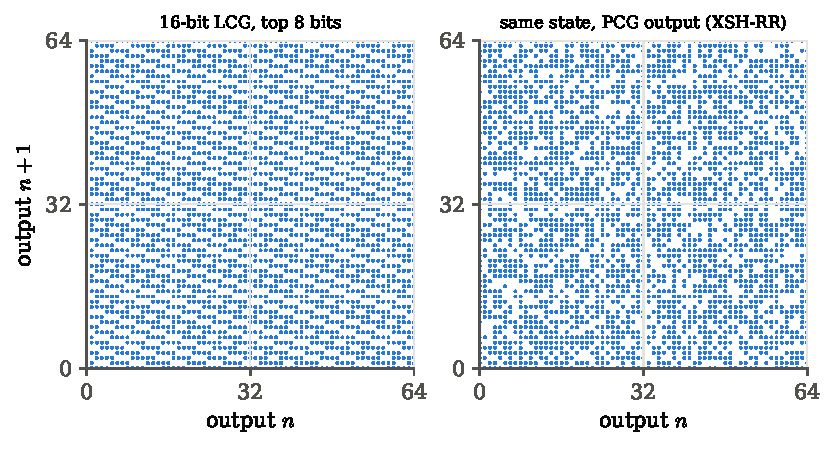
\includegraphics[width=0.85\linewidth]{figures/ch06/pcg_toy.pdf}
\caption{A 16-bit linear congruential state turned into 8-bit outputs in two ways;
each dot is a pair of consecutive outputs (a corner of the full $256\times256$
plot is shown). Left: keeping the top 8 bits; the pairs fall on regular rows, the
lattice of \cref{6a:sec:lattice}. Right: PCG's xorshift-and-rotate output applied
to the same state; the regular rows are gone.}
\label{6a:fig:pcg-toy}
\end{figure}

Counting makes the same point. There are $K=256^2=65536$ possible pairs of
$8$-bit outputs, and one period gives $n=65536$ consecutive pairs. How many
distinct pairs would a truly random sequence of that length produce? Take one
particular pair. A random sequence hits it at least once with probability
\begin{align}
  1-\Bigl(1-\frac1K\Bigr)^{n}
  &\eqby{1}1-\exp\Bigl[n\ln\Bigl(1-\frac1K\Bigr)\Bigr]
   \eqby{2}1-\exp\Bigl[-\frac nK+O\Bigl(\frac n{K^2}\Bigr)\Bigr]
   \eqby{3}1-e^{-1}+O(K^{-1})\approx0.632 .
  \label{6a:eq:coverage}
\end{align}
\begin{explain}
  \item Each of the $n$ pairs misses the given pair with probability $1-1/K$,
        independently; $y^n=e^{n\ln y}$.
  \item $\ln(1-\epsilon)=-\epsilon-\epsilon^2/2-\dots$ with $\epsilon=1/K$.
  \item $n=K$.
\end{explain}
Multiplying by the $K$ possible pairs, about $K(1-e^{-1})\approx41{,}428$
distinct pairs are expected, with a standard deviation of about
$80$ (the variance of the number of empty cells is approximately
$Ke^{-1}(1-2e^{-1})$). The permuted output produces $\SixAPairsPcg$ distinct pairs
($\SixAPairsPcgPct\%$), as expected. The truncated LCG produces $\SixAPairsLcg$
($\SixAPairsLcgPct\%$), about six standard deviations too few: its pairs are too
regular to spread as randomly as random pairs do.

\subsection{Counter-based generators, and a summary}

A different design removes the transition function altogether. A
\newterm{counter-based generator} uses the state $s_n=n$, a plain counter, and puts
all the work into the output: $u_n=g_k(n)$, where $g_k$ is a bijective scramble of
$64$ or $128$ bits controlled by a key $k$, built from a few rounds of a simplified
block cipher \cite{Salmon2011}. Jumping ahead by any amount is free (just set $n$),
and every key gives an independent stream, which suits GPUs where each of thousands
of threads needs its own numbers. Numpy provides one of them as \texttt{Philox}.

\begin{taxonomy}[Generators and what is inside them]
\small
\renewcommand{\arraystretch}{1.12}
\begin{tabularx}{\linewidth}{@{}>{\raggedright\arraybackslash}p{1.9cm}
                               >{\raggedright\arraybackslash}p{1.8cm}
                               >{\raggedright\arraybackslash}X
                               >{\raggedright\arraybackslash}p{1.5cm}
                               >{\raggedright\arraybackslash}p{3.0cm}@{}}
\toprule
generator & state & transition / output & period & known weakness\\\midrule
RANDU & 31 bits & $65539x\bmod2^{31}$ / $x/2^{31}$ & $2^{29}$ & triples on 15 planes\\
MINSTD & 31 bits & $16807x\bmod(2^{31}-1)$ / $x/m$ & $2^{31}-2$ & short period, lattice for $t\gtrsim5$\\
xorshift64 & 64 bits & three shift-XORs / the state & $2^{64}-1$ & linear over bits\\
MT19937 & 19937 bits & linear twist / tempering & $2^{19937}-1$ & linear over bits, predictable\\
PCG64 & 128 + 128 bits & LCG mod $2^{128}$ / XSL-RR & $2^{128}$ per stream & streams with specially related seeds can be correlated\\
Philox & counter + key & $n\mapsto n+1$ / keyed scramble & $2^{256}$ & none known for simulation\\
\bottomrule
\end{tabularx}
\end{taxonomy}

Every modern design splits the work the same way. The transition only needs to
guarantee a long period, which a linear rule, over integers or over bits, does
with a proof. The output function supplies the statistical quality, by mixing the
good and bad parts of the state nonlinearly. Whether the result is good enough is
decided not by the design but by statistical tests (\cref{6a:sec:tests}).
\section{Seeds, streams and reproducible parallel simulations}
\label{6a:sec:seeds}

A realistic Monte Carlo study is not one run but thousands. To estimate the
covariance of a power-spectrum estimator in \cref{ch:08} we will simulate a
thousand skies; a detector study runs the same event simulation on hundreds of
cluster nodes at once. Each job needs its own stream of random numbers. Three
things must be true of these streams. Each must be \emph{reproducible}: if job 417
produced a strange map, we must be able to regenerate exactly that map to find out
why. They must be \emph{different}: two jobs with the same stream would produce the
same sky twice and silently halve our sample. And they must be \emph{unrelated}: no
simple relation between the numbers of different jobs, or the thousand skies are
not a thousand independent draws. So the question is: how do we seed many
streams so that all three hold? The helper \pyname{rng_for}, which makes every
random stream used here, is one answer, and we follow it down to the bits.

\subsection{Why ``seed = job number'' can go wrong}

The obvious recipe is to seed job $j$ with the integer $j$. It is safe only if
the generator forgets where it started. Nearby seeds are nearby states, and some
transitions keep nearby states related forever.

\paragraph{Example: RANDU from the seeds 1 and 3.}
RANDU (\cref{6a:sec:lattice}) is multiplicative: by \eqref{6a:eq:closed},
$x_n=a^nx_0\bmod2^{31}$. Start one stream from $x_0=1$ and another from $x_0'=3$.
Then
\begin{align}
  x'_n
  &\eqby{1}a^n\cdot3\bmod2^{31}
   \eqby{2}3\,x_n\bmod2^{31},
  \qquad\text{so}\qquad
  u'_n\eqby{3}3u_n\bmod1 .
  \label{6a:eq:randu-seeds}
\end{align}
\begin{explain}
  \item The closed form with $c=0$ and seed $3$.
  \item $a^n\cdot3=3\cdot a^n$, and $a^n\equiv x_n$ for the stream from the seed $1$;
        reducing before or after multiplying by $3$ gives the same remainder.
  \item Divide by $2^{31}$: $u'_n=x'_n/2^{31}$ is the fractional part of $3u_n$.
\end{explain}
So the second stream is a fixed function of the first. Each stream on its own is as
good (or as bad) as RANDU, but plotted against each other they lie on three lines
(\cref{6a:fig:streams}, left); the script confirms $u'_n=3u_n\bmod1$ to the last
bit. For any multiplicative generator, the seeds $x_0$ and $kx_0$ give streams
related by multiplication by $k$.

\begin{figure}[htbp]
\centering
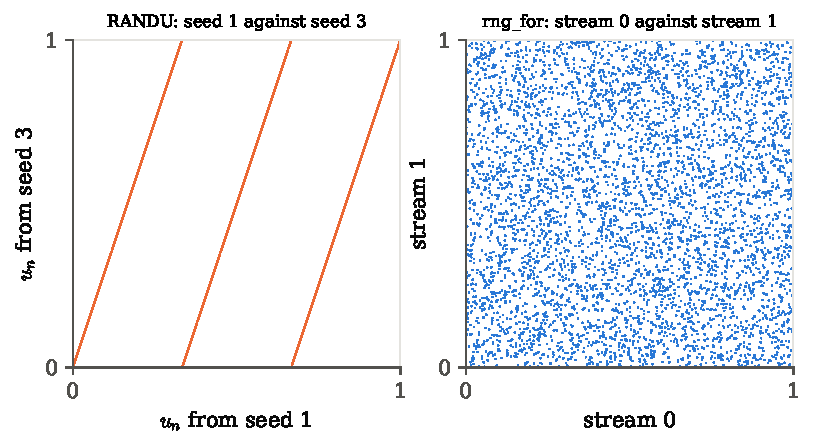
\includegraphics[width=0.8\linewidth]{figures/ch06/streams.pdf}
\caption{Two streams plotted against each other, $5000$ numbers each. Left: RANDU
started from the seeds $1$ and $3$; the second stream is the fractional part of
three times the first, so the points lie on three lines. Right: streams $0$ and
$1$ of \pyname{rng_for} for the same script; no relation is visible.}
\label{6a:fig:streams}
\end{figure}

\paragraph{Example: random 32-bit seeds collide.}
The opposite recipe, a random seed per job, has its own trap if the seed is small.
Many older interfaces accept a 32-bit integer, so there are only $K=2^{32}\approx
4.3\times10^9$ seeds. How likely is it that two of $n$ jobs draw the same one?
This is the birthday problem, with $K$ seeds in place of $365$ days. The chance
that $n$ independently chosen seeds are all different is
\begin{align}
  \Prob(\text{all $n$ seeds different})
  &\eqby{1}\prod_{k=0}^{n-1}\Bigl(1-\frac kK\Bigr)
   \eqby{2}\exp\Bigl[\sum_{k=0}^{n-1}\ln\Bigl(1-\frac kK\Bigr)\Bigr]
   \relby{3}{\approx}\exp\Bigl[-\sum_{k=0}^{n-1}\frac kK\Bigr]
   \eqby{4}\exp\Bigl[-\frac{n(n-1)}{2K}\Bigr] .
  \label{6a:eq:birthday}
\end{align}
\begin{explain}
  \item The $(k+1)$-th seed must avoid the $k$ values already taken, which has
        probability $1-k/K$, independently of the earlier draws.
  \item A product is the exponential of the sum of the logarithms.
  \item $\ln(1-\epsilon)\approx-\epsilon$ for $\epsilon=k/K\ll1$.
  \item $\sum_{k=0}^{n-1}k=n(n-1)/2$.
\end{explain}
With $n=10^3$ jobs a collision has probability $\SixABdayThree$, with $10^4$ jobs
$\SixABdayFour$, and with $10^5$ jobs $\SixABdayFive$: more likely than not, two of
a hundred thousand simulations are identical. The exact product and the
approximation agree to three digits. With $128$-bit seeds and the same $10^5$ jobs
the probability is $\SixABdayOneTwoEight$. Seeds must be long.

\subsection{SeedSequence: hashing a seed into a state}

Numpy solves both problems by never putting a user's seed directly into the
generator's state. A \newterm{SeedSequence} takes any collection of nonnegative
integers as \newterm{entropy} \unpack{here, the numbers that identify the job:
a base seed and a stream index} and mixes them with a hash function into a pool
of $128$ bits. Every input bit affects every pool bit, so the entropies $[s,0]$ and
$[s,1]$, which differ in one bit, give pools that look unrelated. From the pool it
then generates as many state words as the generator needs, again through a hash.
The two problems of the examples disappear: nearby inputs no longer give nearby
states, and the state is drawn from $2^{128}$ or more possibilities. The method
\texttt{spawn(n)} makes $n$ child sequences by appending the child's index to the
entropy, so that a job can in turn seed its own sub-jobs, and the resulting tree of
streams is reproducible from the single root.

The helper \pyname{rng_for} of \pyname{code/common.py} is three lines:

\pyfile[firstline=122,lastline=126,firstnumber=122]{code/common.py}{Every random stream in the book is made here}

Line 124 builds the script's name, e.g.\ \texttt{"ch06/07\_seeds\_streams"} (the optional salt is the
testing switch of \cref{0a:sec:code}; in the book's own runs it is empty). Line 125 turns that name into a
$64$-bit integer: the first eight bytes of its SHA-256 hash. For this script it is
$\SixASeedInt$. The name, not a number typed by hand, is the seed, so two scripts
can never share a stream by accident, and renaming a script is the only way to
change its random numbers. Line 126 feeds $[\text{seed},\text{stream}]$ into a
SeedSequence and hands the result to PCG64. The script \pyname{07_seeds_streams.py}
follows the path down to the bits (\cref{6a:fig:rngfor}):

\pyfile[firstline=36,lastline=44,firstnumber=36]{code/ch06/07_seeds_streams.py}{rng\_for traced by hand: SeedSequence words to the PCG64 state}

Line 37 asks the SeedSequence for four $64$-bit words. The first two become a
$128$-bit starting value (line 38), the last two the stream selector (line 39),
from which line 40 makes the odd increment $c=2\times\text{selector}+1$ of the
linear congruential step of \cref{6a:sec:modern}. Lines 41--44 are PCG's seeding
rule: one step from zero, add the starting value, one more step. The state and
increment obtained this way are identical to the ones inside numpy's generator, and
so are the next $1000$ outputs of the \pyname{PCG64} class of \cref{6a:sec:modern}.
So nothing in the random numbers is hidden: every operation from the name of a
script to its first output is now explicit.

\begin{figure}[htbp]
\centering
\begin{tikzpicture}[
  node distance=5mm and 4mm,
  box/.style={draw=accent,thick,rounded corners=2pt,fill=ideabg,align=center,
              font=\small,minimum height=10mm,text width=23mm},
  flow/.style={->,thick,accent}]
  \node[box] (name) {script name\\ \texttt{"ch06/07\_\dots"}};
  \node[box,right=of name] (hash) {SHA-256,\\ first 8 bytes:\\ 64-bit seed};
  \node[box,right=of hash] (ss) {SeedSequence\\ $[\text{seed},\text{stream}]$\\ $\to$ 128-bit pool};
  \node[box,right=of ss] (words) {4 words\\ of 64 bits};
  \node[box,below=9mm of words] (pcg) {PCG64 state $s$\\ and odd\\ increment $c$};
  \node[box,left=of pcg] (gen) {\texttt{Generator}:\\ \texttt{random}, \texttt{normal},\\ \texttt{integers}, \dots};
  \node[box,left=of gen] (u) {simulation};
  \draw[flow] (name) -- (hash);
  \draw[flow] (hash) -- (ss);
  \draw[flow] (ss) -- (words);
  \draw[flow] (words) -- (pcg);
  \draw[flow] (pcg) -- (gen);
  \draw[flow] (gen) -- (u);
\end{tikzpicture}
\caption{What \pyname{rng_for} does. The script's name is hashed to a 64-bit
seed; the seed and a stream index are mixed by a SeedSequence into a 128-bit pool,
which generates four 64-bit words; these fix the 128-bit state and the odd
increment of PCG64. The \texttt{Generator} object then turns the 64-bit outputs
into numbers of any distribution.}
\label{6a:fig:rngfor}
\end{figure}

\paragraph{Example: eight streams of one script.}
\pyname{rng_for("ch06", "07_seeds_streams", stream=k)} for $k=0,\dots,7$ gives eight
streams. From $10^6$ numbers of each, the script computes all $28$ correlation
coefficients $r$ between pairs of streams. Under independence each $r$ is
approximately Gaussian with mean $0$ and standard deviation
$1/\sqrt N=\SixAStreamInvSqrtN$ (derived in \cref{6a:sec:tests}), so the $28$
values of $r\sqrt N$ should look like $28$ draws from $\Normal(0,1)$. Their
standard deviation is $\SixAStreamZstd$, the largest $\abs r$ is
$\SixAStreamMaxCorr$, and a Kolmogorov--Smirnov test of $\Normal(0,1)$
(\cref{ch:04}) gives $p=\SixAStreamKsP$: no sign of any relation. The right panel of \cref{6a:fig:streams} shows two of
the streams against each other.

\paragraph{How likely is it that two streams overlap?}
Suppose a generator has a single cycle of length $P$ and each of $n$ jobs starts
at an independent random point of it and consumes $L$ numbers. Two jobs overlap if
their starting points are within $L$ of each other. Fix where the first job
starts; the second overlaps it if it starts in a window of $2L$ positions ($L$
before and $L$ after), out of $P$. So one pair overlaps with probability about
$2L/P$. There are $n(n-1)/2$ pairs, so
$\Prob(\text{any overlap})\lesssim n^2L/P$. For $n=10^4$ jobs of $L=10^{12}$
numbers each (a large simulation campaign) and $P=2^{128}\approx3.4\times10^{38}$,
this is $10^{20}/3.4\times10^{38}\approx3\times10^{-19}$. With PCG64 the streams
also have different increments and are therefore different sequences altogether.
Numpy additionally offers \texttt{jumped()}, which advances a PCG64 state by
about $(\phi-1)\,2^{128}$ steps ($\phi$ the golden ratio) as if that many
numbers had been drawn, for the rare case in which non-overlapping blocks of one
single stream are wanted.

\begin{keyidea}[Seeding many simulations]
Seed once, with a long seed (from physical entropy, or from a hash of a name).
Derive every stream from it by a SeedSequence (a stream index, or
\texttt{spawn}), never by adding job numbers to a seed. Record the root seed next
to the results: it is all that is needed to regenerate any simulation exactly.
\end{keyidea}

\subsection{From 64 bits to a floating-point number}

The generator produces integers; a simulation wants $u\in[0,1)$. A double-precision
number has a $53$-bit significand, so numpy keeps the top $53$ of the $64$ output
bits (the best ones) and scales:
\begin{equation}
  u=\bigl\lfloor x/2^{11}\bigr\rfloor\cdot2^{-53}=\frac k{2^{53}},\qquad
  k\in\{0,1,\dots,2^{53}-1\}\ \text{equally likely} .
  \label{6a:eq:double}
\end{equation}
The script checks that numpy's \texttt{random()} is exactly this, and the function
\pyname{to_double} of the library implements it. The values form a grid of spacing
$2^{-53}\approx1.1\times10^{-16}$. The value $u=1$ never occurs. The value $u=0$
occurs, with probability $2^{-53}$: rare, but at $10^9$ draws per second it happens
about once every
\[
  \frac{2^{53}}{10^9\ \text{s}^{-1}}\approx9\times10^{6}\ \text{s}\approx 104\ \text{days}
\]
of computing, which a large campaign easily exceeds. Cowan's generator excluded both
endpoints \srcref{Cowan}{(3.3)}; numpy's includes $0$.

\begin{pitfall}[$\ln u$ with $u=0$]
The recipe $x=-\tau\ln u$ for exponential decay times (inverse-transform sampling, \cref{6b:sec:inverse})
returns $+\infty$ when $u=0$. Use $x=-\tau\ln(1-u)$, whose argument lies in
$(0,1]$, or the library's \texttt{rng.exponential}, which handles this.
\end{pitfall}
\section{Testing a generator: randomness as a null hypothesis}
\label{6a:sec:tests}

A dice manufacturer who wants to know whether its dice are fair does not inspect
the dice; it rolls them many times and checks that the results behave like those of
ideal, unbiased dice \srcref{Lambert}{\S12.2}. A generator is tested the same way.
We cannot prove that a deterministic sequence is random, since it is not; what we
can do is state the property we need as a hypothesis and look for evidence against
it. This is the logic of \cref{ch:04}, applied to a stream of numbers.
\begin{itemize}[itemsep=1pt]
  \item The null hypothesis $H_0$: the numbers $u_1,\dots,u_N$ are independent
        draws from the uniform distribution \eqref{6a:eq:uniform}. As in
        \cref{ch:04}, we take this as the null because it is the case whose
        distribution we know: for truly random uniform numbers we can compute
        the distribution of any statistic built from them.
  \item A test statistic $T(u_1,\dots,u_N)$ that is sensitive to one particular way
        in which $H_0$ could fail: unequal frequencies, correlation between
        neighbours, too many or too few ups and downs, structure in triples.
  \item The p-value: how often truly random numbers would give a value of $T$
        as far out as the one we got, or further in the same direction.
\end{itemize}
A generator ``fails'' a test when the p-value is tiny, and keeps being tiny when
the test is repeated with fresh numbers. So two questions follow. Which
statistics catch which defects? And why must a good generator pass all of them,
while no finite set of them can prove it good?

\subsection{Four tests, each derived}

\paragraph{1. Equal frequencies: the $\chi^2$ test of a histogram.}
The simplest defect is that some values come up more often than others. To look
for it, divide $[0,1)$ into $k$ equal bins and count the numbers $O_j$ that fall
into bin $j$. Under $H_0$ each number lands in bin $j$ with probability $1/k$, independently,
so the expected count is $E=N/k$ and the counts are multinomial. The statistic
\begin{equation}
  X^2=\sum_{j=1}^{k}\frac{(O_j-E)^2}{E}
  \label{6a:eq:chi2}
\end{equation}
is small when the counts are close to their expectation. What value should we
expect under $H_0$? Its mean follows in one line:
\begin{align}
  \E[X^2]
  &\eqby{1}\sum_{j=1}^k\frac{\Var(O_j)}{E}
   \eqby{2}k\,\frac{N\frac1k\bigl(1-\frac1k\bigr)}{N/k}
   \eqby{3}k-1 .
  \label{6a:eq:chi2-mean}
\end{align}
\begin{explain}
  \item $\E[(O_j-E)^2]=\Var(O_j)$ because $E=\E[O_j]$.
  \item Each $O_j$ is binomial with $N$ trials and success probability $1/k$, so
        $\Var(O_j)=N\cdot\frac1k(1-\frac1k)$ (\cref{ch:02}); all $k$ terms are
        equal.
  \item Cancel $N/k$.
\end{explain}
The mean is $k-1$, not $k$, because the counts obey one constraint, $\sum_jO_j=N$:
only $k-1$ of them are free. For large $E$ each $(O_j-E)/\sqrt E$ is nearly
Gaussian, and $X^2$ is then distributed as $\chi^2$ with $k-1$ degrees of freedom,
the goodness-of-fit result of \cref{ch:04}. We use $k=64$ bins, so $H_0$ predicts
$X^2\approx63\pm11$ (the $\chi^2_\nu$ distribution has variance $2\nu$).

\paragraph{2. Neighbours: the serial correlation.}
A generator can have perfect frequencies and still let each number influence the
next. The lag-one \newterm{serial correlation} is the correlation coefficient of the
pairs $(u_i,u_{i+1})$,
\[
  r=\frac{\sum_{i=1}^{N-1}(u_i-\bar u)(u_{i+1}-\bar u)}{\sum_{i=1}^{N}(u_i-\bar u)^2},
\]
with $\bar u$ the mean of the $u_i$. Under $H_0$ the true correlation is $0$, so
the question is how far from $0$ the measured $r$ strays by chance alone. Its
spread is easy to find if we replace $\bar u$ by its expectation $\tfrac12$ (the error this makes is of relative
order $1/N$). Write $v_i=u_i-\tfrac12$, which has mean $0$ and variance $\tfrac1{12}$
(the variance of a uniform variable on an interval of length $1$). Then for the
numerator $S=\sum_iv_iv_{i+1}$,
\begin{align}
  \Var(S)
  &\eqby{1}\sum_i\E[v_i^2v_{i+1}^2]+2\sum_i\E[v_iv_{i+1}\,v_{i+1}v_{i+2}]
   +(\text{terms with no shared index})\nonumber\\
  &\eqby{2}(N-1)\,\E[v^2]^2+2\sum_i\E[v_i]\,\E[v_{i+1}^2]\,\E[v_{i+2}]+0
   \eqby{3}\frac{N-1}{144},
  \label{6a:eq:serial-var}
\end{align}
\begin{explain}
  \item $\E[S]=\sum_i\E[v_i]\E[v_{i+1}]=0$, so $\Var(S)=\E[S^2]$. Expanding the
        square gives products of two terms $v_iv_{i+1}$ and $v_jv_{j+1}$: the
        diagonal ($j=i$), neighbours that share one index ($j=i\pm1$), and pairs
        with no index in common.
  \item Independence factorises every expectation. The diagonal gives
        $\E[v_i^2]\E[v_{i+1}^2]=(\frac1{12})^2$. A shared-index term contains the
        unshared $v_i$ and $v_{i+2}$ once each, and $\E[v]=0$; a term with no shared
        index contains four factors of which at least one appears once, so it
        vanishes too.
  \item $(\frac1{12})^2=\frac1{144}$.
\end{explain}
The denominator is close to its mean $N/12$, so
$\Var(r)\approx\frac{N/144}{(N/12)^2}=\frac1N$. The statistic $z=r\sqrt N$ is
therefore approximately standard normal under $H_0$ (the central limit theorem
applied to $S$), and $\abs z>3$ has probability $0.3\%$.

\paragraph{3. Ups and downs: the runs test.}
Write $+$ when a number is larger than the one before it and $-$ when it is smaller.
A \newterm{run} is a maximal block of equal signs (\cref{6a:fig:runs}). A sequence
that oscillates too regularly has too many runs; one that drifts has too few. How
many runs should independent numbers give? Count the sign changes: the number of
runs is $R=1+$ (number of sign changes), and a sign change happens at
$u_i$ exactly when $u_i$ is the largest or the smallest of the three numbers
$u_{i-1},u_i,u_{i+1}$. Under $H_0$ the six orderings of three independent
continuous numbers are equally likely, and in four of them the middle one is the
largest or the smallest. So
\begin{align}
  \E[R]
  &\eqby{1}1+\sum_{i=2}^{N-1}\Prob(u_i\text{ is a turning point})
   \eqby{2}1+(N-2)\,\frac46
   \eqby{3}\frac{2N-1}{3} .
  \label{6a:eq:runs-mean}
\end{align}
\begin{explain}
  \item $R$ is $1$ plus a sum of indicator variables, one for each interior
        position, and the expectation of an indicator is its probability.
  \item Four of the six equally likely orderings.
  \item $1+\frac{2N-4}{3}=\frac{2N-1}{3}$.
\end{explain}
The variance, $(16N-29)/90$, comes from the same counting done for pairs of
positions (neighbouring turning points are not independent, which is why it is
not simply $N\cdot\frac23\cdot\frac13$). Then $z=(R-\E[R])/\sqrt{\Var R}$ is
approximately standard normal under $H_0$.

\begin{figure}[htbp]
\centering
\begin{tikzpicture}[xscale=0.78,yscale=2.6]
  \def\vals{0.42,0.71,0.88,0.35,0.12,0.64,0.51,0.93,0.27,0.30,0.76,0.05}
  \draw[black!40] (0.5,0) -- (12.5,0);
  \draw[black!40] (0.5,0) -- (0.5,1) node[left,font=\footnotesize,black] {$1$};
  \node[left,font=\footnotesize] at (0.5,0) {$0$};
  \foreach \v [count=\i] in \vals { \coordinate (p\i) at (\i,\v); }
  \foreach \a/\b in {1/2,2/3,5/6,7/8,9/10,10/11} \draw[thick,tangentgreen] (p\a) -- (p\b);
  \foreach \a/\b in {3/4,4/5,6/7,8/9,11/12} \draw[thick,bdryred] (p\a) -- (p\b);
  \foreach \v [count=\i] in \vals { \node[circle,fill,inner sep=1.1pt] at (p\i) {}; \node[font=\scriptsize,below] at (\i,-0.02) {$u_{\i}$}; }
  \foreach \x/\s/\c in {2/{$+\,+$}/tangentgreen,4/{$-\,-$}/bdryred,5.5/{$+$}/tangentgreen,6.5/{$-$}/bdryred,
                        7.5/{$+$}/tangentgreen,8.5/{$-$}/bdryred,10/{$+\,+$}/tangentgreen,11.5/{$-$}/bdryred}
    \node[font=\footnotesize,\c] at (\x,1.12) {\s};
\end{tikzpicture}
\caption{Runs up and down in twelve numbers. Rising steps are green, falling
steps red. The signs of the steps form eight runs ($++$, $--$, $+$, $-$, $+$, $-$,
$++$, $-$), against $\E[R]=(2\cdot12-1)/3\approx7.7$ for independent uniform
numbers.}
\label{6a:fig:runs}
\end{figure}

\paragraph{4. Triples: the $\chi^2$ test in three dimensions.}
A generator can pass every test on single numbers and on neighbouring pairs and
still fail in three dimensions, as RANDU does (\cref{6a:sec:lattice}). To look
there, group the numbers into non-overlapping triples, treat each as a point in
the unit cube, divide the cube into $20^3=8000$ cells and apply \eqref{6a:eq:chi2} to the
cell counts: $X^2$ should be $7999\pm126$. A generator whose triples lie on a few
planes leaves whole cells empty, and $X^2$ becomes huge.

\subsection{Four generators under the four tests}

The script \pyname{08_randomness_tests.py} applies the four tests to $N=999999$
numbers from each of four generators: PCG64, MT19937, RANDU and the small
generator $x\mapsto(1229x+1)\bmod2048$ of \cref{6a:sec:lcg}.
\Cref{6a:tab:tests} lists the statistics and the p-values (two-sided for the
normal statistics, the upper tail for $X^2$).

\begin{table}[htbp]
\centering
\small
\renewcommand{\arraystretch}{1.15}
\begin{tabular}{@{}lcccc@{}}
\toprule
 & histogram $X^2$ & serial $z$ & runs $z$ & triples $X^2$\\
 & ($\nu=63$) & & & ($\nu=7999$)\\\midrule
PCG64   & $\SixATPcgHistStat$ ($p=\SixATPcgHistP$) & $\SixATPcgSerStat$ ($\SixATPcgSerP$) & $\SixATPcgRunsStat$ ($\SixATPcgRunsP$) & $\SixATPcgTriStat$ ($\SixATPcgTriP$)\\
MT19937 & $\SixATMtHistStat$ ($\SixATMtHistP$) & $\SixATMtSerStat$ ($\SixATMtSerP$) & $\SixATMtRunsStat$ ($\SixATMtRunsP$) & $\SixATMtTriStat$ ($\SixATMtTriP$)\\
RANDU   & $\SixATRanduHistStat$ ($\SixATRanduHistP$) & $\SixATRanduSerStat$ ($\SixATRanduSerP$) & $\SixATRanduRunsStat$ ($\SixATRanduRunsP$) & $\SixATRanduTriStat$ ($\SixATRanduTriP$)\\
LCG, $m=2048$ & $\SixATLamHistStat$ ($\SixATLamHistP$) & $\SixATLamSerStat$ ($\SixATLamSerP$) & $\SixATLamRunsStat$ ($\SixATLamRunsP$) & $\SixATLamTriStat$ ($\SixATLamTriP$)\\
\bottomrule
\end{tabular}
\caption{Four tests of $H_0$ (independent and uniform) on $999999$ numbers from
each generator. Entries are the statistic and, in brackets, its p-value.}
\label{6a:tab:tests}
\end{table}

\paragraph{Reading the table.}
PCG64 and MT19937 pass everything: every statistic is where $H_0$ puts it, and the
p-values are unremarkable numbers between $0$ and $1$. RANDU passes the first three
tests just as well. Its frequencies are uniform, its neighbours uncorrelated, its
runs normal, which is why it was used for years. The triple test destroys it:
$X^2=\SixATRanduTriStat$ where $7999\pm126$ was expected, because its triples occupy
only fifteen planes of the cube (\cref{6a:fig:randu}). The small generator fails in
a way that deserves a second look. Its serial correlation is $z=\SixATLamSerStat$,
i.e.\ $r\approx0.2$: its pairs lie on the six lines of slope $\tfrac15$ in
\cref{6a:fig:lcg-pairs}, so $u_{n+1}$ tends to rise with $u_n$ with slope about
$\tfrac15$. Its runs and triples fail as badly. And its histogram is \emph{too
good}: $X^2=\SixATLamHistStat$ where $63\pm11$ was expected. Over each full period
the generator visits every one of its $2048$ states exactly once, so each of the
$64$ bins gets exactly $32$ numbers per period; the counts have none of the
multinomial scatter that independent numbers would have. The upper-tail p-value is
$1$, but the lower tail tells the story: under $H_0$ an $X^2$ this small has
probability $\SixATLamHistLowP$. A fit that is too good is as much evidence against
$H_0$ as one that is too bad.

The p-value is itself a random variable, and under $H_0$ it is uniformly
distributed on $[0,1]$. The reason is that the p-value is the distribution
function of the statistic evaluated at the statistic, and a continuous random
variable pushed through its own distribution function is uniform (the fact behind
inverse-transform sampling, \cref{6b:sec:pit}). So a good generator gives p-values
spread evenly over $[0,1]$, and a p-value of $0.01$ appears once in a hundred
tests. The left panel of \cref{6a:fig:tests} checks this for
$\SixATreps$ histogram tests on fresh batches of $10^4$ PCG64 numbers; a
Kolmogorov--Smirnov test of their uniformity gives $p=\SixATksP$. The right panel
shows where the triple statistics of the table fall relative to the $\chi^2_{7999}$
density.

\begin{figure}[htbp]
\centering
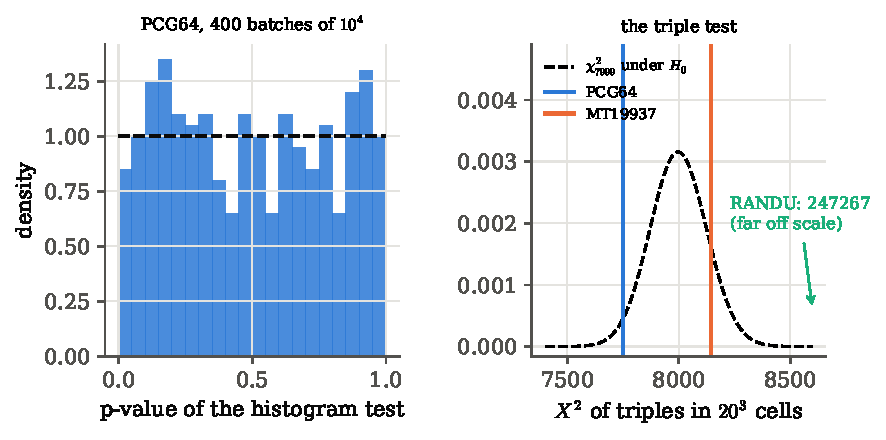
\includegraphics[width=0.9\linewidth]{figures/ch06/tests_pvalues.pdf}
\caption{Left: the p-values of $400$ histogram tests on independent batches of
PCG64 numbers are spread uniformly over $[0,1]$, as they must be under $H_0$.
Right: the triple statistic $X^2$ for PCG64 and MT19937 (vertical lines) sits
inside its $\chi^2_{7999}$ density under $H_0$ (dashed); RANDU's value, about thirty
times larger, is far off the scale.}
\label{6a:fig:tests}
\end{figure}

\begin{pitfall}[One small p-value is not a failure]
Run a hundred tests on a perfect generator and about one will give $p<0.01$. A
defect shows itself as a p-value that is small again and again with fresh numbers,
or that becomes smaller as $N$ grows (for a real defect the statistic grows with
$N$). Conversely, passing a test says only that this particular defect, at this
sample size, is absent.
\end{pitfall}

\subsection{Batteries of tests}

Serious testing uses hundreds of statistics, each designed around a way in which
real generators have failed: gaps between repeated values (birthday spacings),
matrix ranks and linear complexity of the output bits (the tests that catch
xorshift and the Mersenne Twister, \cref{6a:sec:modern}), random walks, the
collision counts of many balls in many cells, and so on. The standard collection is
TestU01 \cite{LEcuyerSimard2007}, organised in three batteries of increasing size
and running time: SmallCrush (minutes), Crush and BigCrush (hours, more than a
hundred test statistics on about $2^{38}$ numbers). Its authors ran it on the
generators in common use in 2007: the power-of-two linear congruential generators
and RANDU fail the smaller batteries, MT19937 passes BigCrush except for the
two linear-complexity tests, and several generators then shipping in popular
software failed badly. PCG64 passes BigCrush \cite{ONeill2014}.

What no battery can do is certify a generator for \emph{every} application. Each
test is a single statistic, and a deterministic sequence always has some statistic
that exposes it (for instance ``replay the generator from the seed and compare'').
The practical rules that follow are simple: use a modern generator that passes
BigCrush; never use the low bits of a power-of-two linear congruential generator;
and for a result that matters, repeat the simulation with a second generator of an
unrelated design (numpy offers PCG64, MT19937, Philox and SFC64 behind the same
interface) and check that the answer does not change. That last check would have
caught the Monty Hall failure of \cref{6a:sec:monty} at once.
\section{When randomness is not the point: quasi-random numbers}
\label{6a:sec:qmc}

Return to the oldest use of random numbers in this chapter: an integral
$I=\int h(x)\,\dd x$ over the unit cube $[0,1]^d$, estimated by the
average of $h$ at $N$ uniform points \mainref{p.~404, (24.2)}. The error of that
average falls as $\sigma/\sqrt N$ (derived in \cref{6b:sec:sqrtN}), with
$\sigma$ the standard deviation of $h(X)$ for a uniform point $X$. For an integral,
independence costs us accuracy. Independent points clump by chance and leave gaps
by chance, and the $1/\sqrt N$ is exactly
the size of those chance fluctuations. For an integral we do not need points that
are unpredictable. We need points that cover the cube evenly. A regular grid does
that, but in $d$ dimensions it needs $n^d$ points for $n$ per axis, and it cannot be
extended one point at a time. So the question is: are there point sets that can
be extended one point at a time and still fill the cube more evenly than chance?
And if so, how much accuracy does that buy?

\subsection{Van der Corput and Sobol sequences}

In one dimension there is a simple construction. Write $n=1,2,3,\dots$ in
binary and mirror the digits about the binary point: $n=(b_k\dots b_2b_1)_2$
becomes $\phi(n)=(0.b_1b_2\dots b_k)_2$, the \newterm{radical inverse} of $n$.
For example,
\begin{align}
  \phi(6)
  &\eqby{1}\phi\bigl((110)_2\bigr)
   \eqby{2}(0.011)_2
   \eqby{3}0\cdot\tfrac12+1\cdot\tfrac14+1\cdot\tfrac18
   =\tfrac38 .
  \label{6a:eq:vdc}
\end{align}
\begin{explain}
  \item $6=4+2=(110)_2$.
  \item Read the digits from the right, after the binary point.
  \item The $i$-th digit after the point is worth $2^{-i}$.
\end{explain}
The \newterm{van der Corput sequence} $\phi(1),\phi(2),\dots$ begins
$\tfrac12$, $\tfrac14$, $\tfrac34$, $\tfrac18$, $\tfrac58$, $\tfrac38$, $\tfrac78$, $\tfrac1{16}$, \dots
(the script \pyname{09_sobol.py} prints the first eight). Every new point lands in
a largest gap left by the earlier ones (\cref{6a:fig:vdc}): after $2^m$ points,
each interval $[j/2^m,(j+1)/2^m)$ contains exactly one of them. Why does mirroring
the digits do this? The last binary digit of $n$ alternates fastest, and it becomes the first digit of $\phi(n)$, so
consecutive points jump between the two halves of the interval; the next digit
chooses the quarter, and so on.

\begin{figure}[htbp]
\centering
\begin{tikzpicture}[x=10cm,y=3cm]
  \draw[thick,black!60] (0,0) -- (1,0);
  \foreach \x in {0,1} \draw[black!60] (\x,0.1) -- (\x,-0.1) node[below,font=\footnotesize] {$\x$};
  \foreach \v/\n/\y in {0.5/1/0.95,0.25/2/0.8,0.75/3/0.8,0.125/4/0.65,0.625/5/0.65,
                        0.375/6/0.65,0.875/7/0.65,0.0625/8/0.5} {
    \draw[formblue!60] (\v,0) -- (\v,\y);
    \fill[fibreorange!85!black] (\v,\y) circle (1.6pt);
    \node[font=\footnotesize,anchor=south] at (\v,\y+0.03) {$\n$};
  }
  \node[font=\footnotesize,anchor=west] at (1.02,0.95) {$n=1$};
  \node[font=\footnotesize,anchor=west] at (1.02,0.8) {$n=2,3$};
  \node[font=\footnotesize,anchor=west] at (1.02,0.65) {$n=4,\dots,7$};
  \node[font=\footnotesize,anchor=west] at (1.02,0.5) {$n=8$};
\end{tikzpicture}
\caption{The first eight points of the van der Corput sequence, drawn at a height
that marks the generation they belong to. The first point halves the interval,
the next two halve the halves, the next four halve the quarters. After $2^m$
points every interval of length $2^{-m}$ holds exactly one point.}
\label{6a:fig:vdc}
\end{figure}

Sobol generalised this to $d$ dimensions \cite{Sobol1967}. Coordinate $j$ of the
$n$-th point is built from the binary digits $b_1,b_2,\dots$ of $n$ as
$x_{n,j}=b_1v_{j,1}\oplus b_2v_{j,2}\oplus\cdots$, an XOR of fixed binary fractions
$v_{j,i}$, the \newterm{direction numbers} of coordinate $j$. For the first
coordinate $v_{1,i}=2^{-i}$, which is the van der Corput sequence; for the others
the direction numbers are derived from different primitive polynomials over the
bits, chosen so that the coordinates do not line up. The result is a
\newterm{digital net}: the first $2^m$ points of a two-dimensional Sobol sequence
have exactly one point in every rectangle $[a2^{-i},(a+1)2^{-i})\times
[b2^{i-m},(b+1)2^{i-m})$, for every $i=0,\dots,m$. With $m=8$ and $i=4$, every cell of
a $16\times16$ grid contains exactly one of the first $256$ points. Independent
points do not do this: the chance that a given cell is empty is
$(1-\frac1{256})^{256}\approx e^{-1}$, so about $\SixAEmptyExpected$ of the $256$
cells should be empty. In \cref{6a:fig:sobol-points}, $256$ PCG64 points leave
$\SixAEmptyPcg$ cells empty and $256$ Sobol points leave $\SixAEmptySobol$.

\begin{figure}[htbp]
\centering
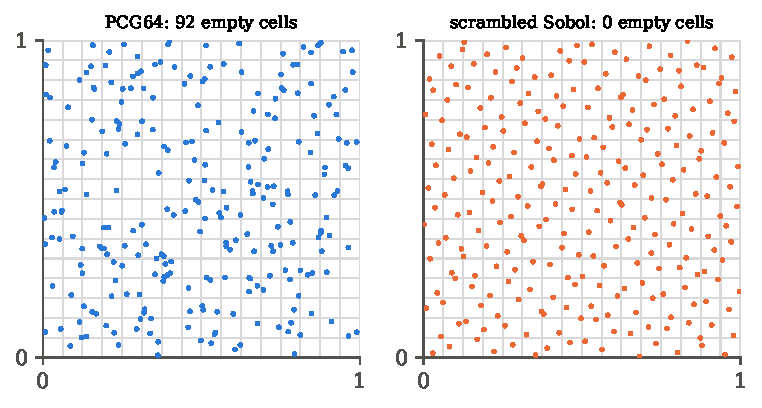
\includegraphics[width=0.8\linewidth]{figures/ch06/sobol_points.pdf}
\caption{256 points in the unit square with a $16\times16$ grid. Left: independent
uniform points from PCG64, which clump and leave about a third of the cells empty.
Right: the first 256 points of a scrambled Sobol sequence, exactly one per cell.}
\label{6a:fig:sobol-points}
\end{figure}

\subsection{Why even points integrate better}

Why should evenly spread points give a smaller error? To answer this we first need
a number for how evenly $N$ points cover the cube. That number is the
\newterm{star discrepancy}
\[
  D_N^*=\sup_{\bm y\in[0,1]^d}\;\Bigl|\,\frac{\#\{i:\ \bm x_i\in[\bm0,\bm y)\}}N-y_1y_2\cdots y_d\,\Bigr|,
\]
the worst difference, over all boxes with one corner at the origin, between the
fraction of points in the box and the volume of the box. In one dimension it has a
simple meaning: $D_N^*=\sup_y\abs{F_N(y)-y}$, the largest gap between the
\newterm{empirical distribution function} $F_N(y)$ \unpack{the fraction of the
points below $y$} and the uniform distribution function $y$, which is the
Kolmogorov--Smirnov statistic of \cref{ch:04}. The answer to our question is that
the integration error is bounded by the discrepancy. In one dimension, for a function $h$ with a continuous derivative,
\begin{align}
  \frac1N\sum_{i=1}^Nh(x_i)-\int_0^1h(x)\,\dd x
  &\eqby{1}\int_0^1h(x)\,\dd\bigl[F_N(x)-x\bigr]\nonumber\\
  &\eqby{2}\Bigl[h(x)\bigl(F_N(x)-x\bigr)\Bigr]_0^1-\int_0^1\bigl(F_N(x)-x\bigr)\,h'(x)\,\dd x
   \nonumber\\
  &\eqby{3}-\int_0^1\bigl(F_N(x)-x\bigr)\,h'(x)\,\dd x ,
  \nonumber\\
  \Bigl|\frac1N\sum_{i=1}^Nh(x_i)-\int_0^1h\,\dd x\Bigr|
  &\relby{4}{\le}\ \sup_x\abs{F_N(x)-x}\int_0^1\abs{h'(x)}\,\dd x
   \eqby{5}D_N^*\;V(h) .
  \label{6a:eq:koksma}
\end{align}
\begin{explain}
  \item $F_N$ jumps by $1/N$ at each point, so integrating against $\dd F_N$ gives
        the average $\frac1N\sum h(x_i)$; integrating against $\dd x$ gives the
        integral (a Stieltjes integral is just this bookkeeping).
  \item Integration by parts.
  \item At $x=0$, $F_N(0)=0$ (no point lies below $0$); at $x=1$, $F_N(1)=1$. Both
        boundary terms vanish.
  \item Bound the integrand by the largest value of $\abs{F_N-x}$ times $\abs{h'}$.
  \item $V(h)=\int_0^1\abs{h'}\dd x$ is the total variation of $h$, how much it goes
        up and down.
\end{explain}
The error is a product of two factors, one belonging to the integrand (its
variation) and one belonging to the points (their discrepancy). In $d$ dimensions
the same statement, with a suitable multidimensional variation $V_{\rm HK}(h)$, is the
\newterm{Koksma--Hlawka inequality}, $\abs{\text{error}}\le V_{\rm HK}(h)\,D_N^*$.

\begin{keyidea}[Discrepancy against chance]
For independent uniform points the discrepancy, like any Kolmogorov--Smirnov
statistic, shrinks only as $N^{-1/2}$. For a Sobol sequence it shrinks as
$(\ln N)^d/N$. For an integrand of bounded variation the Monte Carlo error
$\propto N^{-1/2}$ is therefore replaced by a quasi-Monte Carlo error of order
$(\ln N)^d/N$, which for moderate $d$ and practical $N$ behaves close to $N^{-1}$.
\end{keyidea}

\paragraph{Example: a smooth integrand and one with a jump, in five dimensions.}
Take $d=5$ and two integrands with known integrals: the smooth product
$h(\bm x)=\prod_{i=1}^5\frac\pi2\sin\pi x_i$, whose integral is $1$ (each factor
integrates to $\frac\pi2\cdot\frac2\pi=1$), and the indicator of the ball of radius
$\tfrac12$ about the centre of the cube, whose integral is the ball's volume
$\pi^{5/2}(\tfrac12)^5/\Gamma(\tfrac72)=\SixABallVol$. For $N=2^4,\dots,2^{16}$ the
script estimates both with PCG64 points and with scrambled Sobol points, repeats
everything $\SixASobolR$ times with independent randomisations, and plots the
root-mean-square error (\cref{6a:fig:sobol-error}). With PCG64 both errors fall with
slope $\SixASlopeSmoothMc$ on the log--log plot, the $N^{-1/2}$ law. With Sobol
points the smooth integrand's error falls with slope $\SixASlopeSmoothSob$, and at
$N=2^{16}$ it is $\SixAGainSmooth$ times smaller than the Monte Carlo error; to get
the same accuracy by Monte Carlo would need about $\SixAGainSmooth^2\approx2\times10^4$
times more points. For the ball the slope is only $\SixASlopeBallSob$ and the gain a
factor $\SixAGainBall$. The indicator of a ball has a jump across a curved surface,
and its Hardy--Krause variation is infinite for $d\ge2$, so the Koksma--Hlawka bound
gives nothing; the points still help a little, because the part of the cube away
from the surface is integrated well.

\begin{figure}[htbp]
\centering
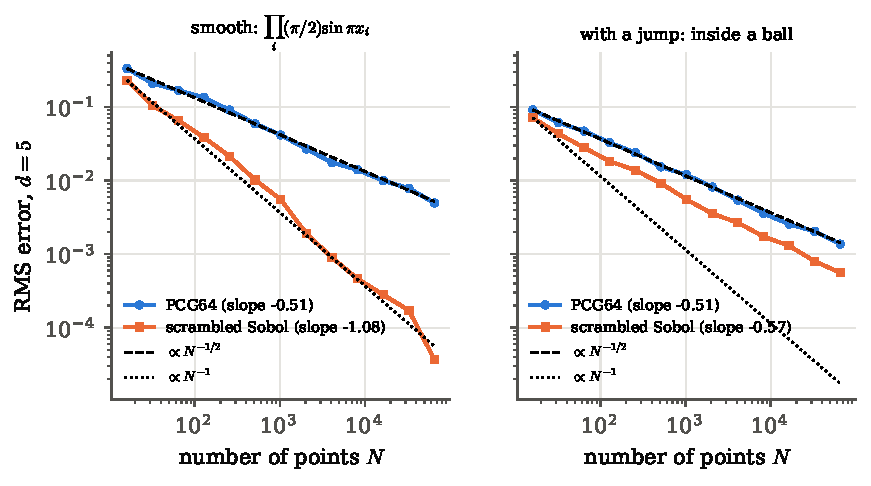
\includegraphics[width=0.95\linewidth]{figures/ch06/sobol_error.pdf}
\caption{Root-mean-square error of the estimate of a five-dimensional integral
against the number of points, over 40 independent randomisations. Left: a smooth
integrand; the Sobol error (orange) falls about as $N^{-1}$ (dotted), the Monte
Carlo error (blue) as $N^{-1/2}$ (dashed). Right: the indicator of a ball, which
has a jump; the Sobol points gain only a constant factor.}
\label{6a:fig:sobol-error}
\end{figure}

Without randomisation a quasi-random estimate has no error bar. An unscrambled
Sobol sequence is deterministic, and its error, though small, cannot be estimated
from the points themselves: the $N$ points are not independent, so the
formula $s/\sqrt N$ does not apply. \newterm{Scrambling} applies random
permutations to the binary digits of every coordinate in a way that keeps the net
property of \cref{6a:fig:sobol-points} but makes each individual point uniform on the
cube. The estimate is then unbiased, and $R$ independent scramblings give $R$
independent estimates whose scatter is an honest error bar. This is how the RMS
errors in \cref{6a:fig:sobol-error} were measured.

\paragraph{Quasi-random points are not random numbers.}
Sobol points are built to be as dependent as possible, each one filling the gaps
left by the others. Used where independence matters (Monty's coin, the steps of a
random walk, the proposals and acceptance tests of MCMC in \cref{ch:09}) they give
wrong answers. They replace a generator only in the estimation of an integral,
where the dimension $d$ is the number of uniform numbers used per sample.

\begin{inpractice}[Random numbers in research code]
\emph{Generators.} Research code in Python uses \texttt{numpy.random.default\_rng}
(PCG64) or, for massively parallel work, \texttt{PCG64DXSM} or \texttt{Philox}.
Detector simulation with Geant4 uses the MixMax generator of the CLHEP library by
default; Pythia 8 uses its own implementation of the Marsaglia--Zaman--Tsang
generator; lattice field theory codes traditionally use L\"uscher's RANLUX, whose
``luxury level'' trades speed for proven decorrelation. The old warnings
(\cref{6a:sec:lcg,6a:sec:lattice}) concern code that still calls C's \texttt{rand()}
or a home-made linear congruential generator.

\emph{Seeds.} A simulation campaign has one root seed, recorded with the outputs;
every job derives its stream from it with \texttt{SeedSequence.spawn} or a job
index, as \pyname{rng_for} does. Cosmological simulation suites store the seed of
every realisation, so that any single CMB map or $N$-body initial condition can be
regenerated exactly when it turns out to be an outlier.

\emph{Verification and research.} Every numerical experiment with generators so far
\emph{verified} something we could also compute: the Monty Hall posterior, $\pi$,
integrals with known values, lattice planes derived by hand. That is the right
way to validate a generator. In research the same machinery becomes the instrument:
the covariance of a masked, noisy power-spectrum estimator in \cref{ch:08} has no
formula, and its only definition is a histogram over simulations. There the
generator's quality can no longer be checked against an answer, and the rules
above (a modern generator, long seeds, SeedSequence streams, a rerun with a
second generator) are what make the result trustworthy. Quasi-Monte Carlo is used
where the integrand is smooth and moderately low-dimensional: option pricing in
finance, radiative-transfer and rendering integrals, and phase-space integration
of smooth matrix elements, for which scrambled Sobol points are available as
\texttt{scipy.stats.qmc.Sobol}.
\end{inpractice}

Every simulation rests on one object: a stream of numbers that must behave like
independent uniform draws on $[0,1)$. Such a stream comes from a deterministic
state machine, so its quality is a property we test, and its seeds and streams are
choices we record. Uniform numbers can then be turned into draws from any
distribution (\cref{6b:sec:inverse}), and averages over those draws into estimates
with an error we can quote (\cref{6b:sec:sqrtN}).

\begin{recap}
\begin{itemize}[itemsep=1pt]
  \item A simulation reproduces probabilities as frequencies, so it is only as good
        as its random numbers: a coin taken from the lowest bit of a linear
        congruential generator changed Monty's $\Prob(E\given H_A)$ from $\tfrac12$
        to $0$ or $1$, and with it the posterior.
  \item A pseudorandom number generator is a deterministic state machine (state,
        transition, output, seed). Finite state forces a period; after it the
        estimate stops improving while the reported error bar keeps shrinking.
  \item Linear congruential generators $x\mapsto(ax+c)\bmod m$: period $m$ under the
        Hull--Dobell conditions, the order of $a$ for prime $m$; the low $j$ bits of
        a power-of-two modulus have period $2^j$.
  \item Their $t$-tuples lie on hyperplanes $\bm h\cdot\bm u\in\Z$ for every dual
        vector $\bm h$; RANDU's triples lie on $15$ planes
        ($9u_n-6u_{n+1}+u_{n+2}\in\Z$). The spectral test measures the widest gap
        $d_t=1/\nu_t$; Marsaglia's bound allows at most $(t!\,m)^{1/t}$ planes.
  \item Modern generators separate a cheap long-period transition (xorshift and
        MT19937, linear over bits; the 128-bit LCG of PCG64) from a mixing output
        function (tempering; XSL-RR). Our ten-line PCG64 reproduces numpy's bits.
  \item Seeds: long, hashed through a SeedSequence, one root recorded; streams by
        index or spawn. Numpy's doubles are $k/2^{53}$ and can be $0$.
  \item Testing: $H_0$ = independent and uniform. Histogram $\chi^2$, serial
        correlation ($\Var r\approx1/N$), runs ($\E R=(2N-1)/3$), triples;
        RANDU passes three and fails the fourth; too good a fit also rejects $H_0$.
  \item Quasi-random (Sobol) points fill space evenly; for smooth integrands the
        error falls close to $N^{-1}$ instead of $N^{-1/2}$ (Koksma--Hlawka), but they
        are not random numbers.
\end{itemize}
\end{recap}
\providecommand{\SixBInvN}{}\renewcommand{\SixBInvN}{100000}
\providecommand{\SixBInvTmean}{}\renewcommand{\SixBInvTmean}{2.196}
\providecommand{\SixBInvTstd}{}\renewcommand{\SixBInvTstd}{2.203}
\providecommand{\SixBInvTse}{}\renewcommand{\SixBInvTse}{0.006967}
\providecommand{\SixBInvNE}{}\renewcommand{\SixBInvNE}{1000000}
\providecommand{\SixBInvFracTeV}{}\renewcommand{\SixBInvFracTeV}{3.940\times10^{-4}}
\providecommand{\SixBInvExactTeV}{}\renewcommand{\SixBInvExactTeV}{3.981\times10^{-4}}
\providecommand{\SixBInvCountTeV}{}\renewcommand{\SixBInvCountTeV}{394}
\providecommand{\SixBInvEmax}{}\renewcommand{\SixBInvEmax}{4.31e+04}
\providecommand{\SixBInvCumZero}{}\renewcommand{\SixBInvCumZero}{0.01978}
\providecommand{\SixBInvCumOne}{}\renewcommand{\SixBInvCumOne}{0.1516}
\providecommand{\SixBInvCumTwo}{}\renewcommand{\SixBInvCumTwo}{0.4812}
\providecommand{\SixBInvCumThree}{}\renewcommand{\SixBInvCumThree}{0.8474}
\providecommand{\SixBInvPoisMean}{}\renewcommand{\SixBInvPoisMean}{3.499}
\providecommand{\SixBInvPoisVar}{}\renewcommand{\SixBInvPoisVar}{3.546}
\providecommand{\SixBInvBinMax}{}\renewcommand{\SixBInvBinMax}{0.001509}
\providecommand{\SixBBmN}{}\renewcommand{\SixBBmN}{100000}
\providecommand{\SixBBmMeanX}{}\renewcommand{\SixBBmMeanX}{3.503\times10^{-4}}
\providecommand{\SixBBmVarX}{}\renewcommand{\SixBBmVarX}{1.006}
\providecommand{\SixBBmMeanY}{}\renewcommand{\SixBBmMeanY}{9.210\times10^{-4}}
\providecommand{\SixBBmVarY}{}\renewcommand{\SixBBmVarY}{1.001}
\providecommand{\SixBBmCorr}{}\renewcommand{\SixBBmCorr}{0.003211}
\providecommand{\SixBBmRsqMean}{}\renewcommand{\SixBBmRsqMean}{2.007}
\providecommand{\SixBBmKS}{}\renewcommand{\SixBBmKS}{0.9435}
\providecommand{\SixBBmKurt}{}\renewcommand{\SixBBmKurt}{3.054}
\providecommand{\SixBBmPolarAcc}{}\renewcommand{\SixBBmPolarAcc}{0.7847}
\providecommand{\SixBBmPolarVar}{}\renewcommand{\SixBBmPolarVar}{1.004}
\providecommand{\SixBChLa}{}\renewcommand{\SixBChLa}{1.6}
\providecommand{\SixBChLb}{}\renewcommand{\SixBChLb}{1.2}
\providecommand{\SixBChSxx}{}\renewcommand{\SixBChSxx}{1.006}
\providecommand{\SixBChSxy}{}\renewcommand{\SixBChSxy}{1.609}
\providecommand{\SixBChSyy}{}\renewcommand{\SixBChSyy}{4.011}
\providecommand{\SixBChRho}{}\renewcommand{\SixBChRho}{0.8009}
\providecommand{\SixBChN}{}\renewcommand{\SixBChN}{200}
\providecommand{\SixBChM}{}\renewcommand{\SixBChM}{4000}
\providecommand{\SixBChEll}{}\renewcommand{\SixBChEll}{2}
\providecommand{\SixBChMaxDev}{}\renewcommand{\SixBChMaxDev}{0.06748}
\providecommand{\SixBChExpDev}{}\renewcommand{\SixBChExpDev}{0.02236}
\providecommand{\SixBChCfAtEll}{}\renewcommand{\SixBChCfAtEll}{0.3608}
\providecommand{\SixBChCfBadAtEll}{}\renewcommand{\SixBChCfBadAtEll}{0.746}
\providecommand{\SixBRjN}{}\renewcommand{\SixBRjN}{200000}
\providecommand{\SixBRjMuAcc}{}\renewcommand{\SixBRjMuAcc}{0.6666}
\providecommand{\SixBRjMuMeanSq}{}\renewcommand{\SixBRjMuMeanSq}{0.399}
\providecommand{\SixBRjHnM}{}\renewcommand{\SixBRjHnM}{1.315}
\providecommand{\SixBRjHnInvM}{}\renewcommand{\SixBRjHnInvM}{0.7602}
\providecommand{\SixBRjHnAcc}{}\renewcommand{\SixBRjHnAcc}{0.7601}
\providecommand{\SixBRjHnMean}{}\renewcommand{\SixBRjHnMean}{0.7978}
\providecommand{\SixBRjHnExactMean}{}\renewcommand{\SixBRjHnExactMean}{0.7979}
\providecommand{\SixBRjTrialsMean}{}\renewcommand{\SixBRjTrialsMean}{1.316}
\providecommand{\SixBRjBetaC}{}\renewcommand{\SixBRjBetaC}{2.67}
\providecommand{\SixBRjBetaAcc}{}\renewcommand{\SixBRjBetaAcc}{0.3729}
\providecommand{\SixBRjBetaInvC}{}\renewcommand{\SixBRjBetaInvC}{0.3746}
\providecommand{\SixBRjBetaMean}{}\renewcommand{\SixBRjBetaMean}{0.3}
\providecommand{\SixBRjBetaExactMean}{}\renewcommand{\SixBRjBetaExactMean}{0.3}
\providecommand{\SixBMcCubeN}{}\renewcommand{\SixBMcCubeN}{10000}
\providecommand{\SixBMcCube}{}\renewcommand{\SixBMcCube}{0.2509}
\providecommand{\SixBMcCubeSe}{}\renewcommand{\SixBMcCubeSe}{0.002818}
\providecommand{\SixBMcCubeSig}{}\renewcommand{\SixBMcCubeSig}{0.2835}
\providecommand{\SixBMcSlope}{}\renewcommand{\SixBMcSlope}{-0.5014}
\providecommand{\SixBMcRmsRatio}{}\renewcommand{\SixBMcRmsRatio}{0.9852}
\providecommand{\SixBMcPhiFour}{}\renewcommand{\SixBMcPhiFour}{0.9761}
\providecommand{\SixBMcPhiSeFour}{}\renewcommand{\SixBMcPhiSeFour}{0.001527}
\providecommand{\SixBMcPhiFive}{}\renewcommand{\SixBMcPhiFive}{0.9775}
\providecommand{\SixBMcPhiSeFive}{}\renewcommand{\SixBMcPhiSeFive}{4.691\times10^{-4}}
\providecommand{\SixBMcPhiExact}{}\renewcommand{\SixBMcPhiExact}{0.9772}
\providecommand{\SixBMcSigOne}{}\renewcommand{\SixBMcSigOne}{0.4834}
\providecommand{\SixBMcSigEight}{}\renewcommand{\SixBMcSigEight}{2.09}
\providecommand{\SixBMcGridErrOne}{}\renewcommand{\SixBMcGridErrOne}{1.028\times10^{-13}}
\providecommand{\SixBMcMcErrOne}{}\renewcommand{\SixBMcMcErrOne}{3.418\times10^{-4}}
\providecommand{\SixBMcNptsOne}{}\renewcommand{\SixBMcNptsOne}{2000000}
\providecommand{\SixBMcGridErrTwo}{}\renewcommand{\SixBMcGridErrTwo}{4.114\times10^{-7}}
\providecommand{\SixBMcMcErrTwo}{}\renewcommand{\SixBMcMcErrTwo}{5.110\times10^{-4}}
\providecommand{\SixBMcNptsTwo}{}\renewcommand{\SixBMcNptsTwo}{1999396}
\providecommand{\SixBMcGridErrFour}{}\renewcommand{\SixBMcGridErrFour}{0.002437}
\providecommand{\SixBMcMcErrFour}{}\renewcommand{\SixBMcMcErrFour}{0.001697}
\providecommand{\SixBMcNptsFour}{}\renewcommand{\SixBMcNptsFour}{456976}
\providecommand{\SixBMcGridErrEight}{}\renewcommand{\SixBMcGridErrEight}{0.09592}
\providecommand{\SixBMcMcErrEight}{}\renewcommand{\SixBMcMcErrEight}{0.001612}
\providecommand{\SixBMcNptsEight}{}\renewcommand{\SixBMcNptsEight}{1679616}
\providecommand{\SixBMcDeltaN}{}\renewcommand{\SixBMcDeltaN}{100000}
\providecommand{\SixBMcDeltaMean}{}\renewcommand{\SixBMcDeltaMean}{-0.1667}
\providecommand{\SixBMcDeltaLo}{}\renewcommand{\SixBMcDeltaLo}{-0.5134}
\providecommand{\SixBMcDeltaHi}{}\renewcommand{\SixBMcDeltaHi}{0.1967}
\providecommand{\SixBMcDeltaPneg}{}\renewcommand{\SixBMcDeltaPneg}{0.8196}
\providecommand{\SixBMcDeltaSe}{}\renewcommand{\SixBMcDeltaSe}{5.748\times10^{-4}}
\providecommand{\SixBAcN}{}\renewcommand{\SixBAcN}{1000000}
\providecommand{\SixBAcCubeD}{}\renewcommand{\SixBAcCubeD}{5}
\providecommand{\SixBAcCube}{}\renewcommand{\SixBAcCube}{0.1668}
\providecommand{\SixBAcCubeExact}{}\renewcommand{\SixBAcCubeExact}{0.1667}
\providecommand{\SixBAcCubeSe}{}\renewcommand{\SixBAcCubeSe}{3.728\times10^{-4}}
\providecommand{\SixBAcCubePull}{}\renewcommand{\SixBAcCubePull}{0.473}
\providecommand{\SixBAcFarD}{}\renewcommand{\SixBAcFarD}{10}
\providecommand{\SixBAcFar}{}\renewcommand{\SixBAcFar}{0.06375}
\providecommand{\SixBAcFarExact}{}\renewcommand{\SixBAcFarExact}{0.06409}
\providecommand{\SixBAcFarSe}{}\renewcommand{\SixBAcFarSe}{2.443\times10^{-4}}
\providecommand{\SixBAcFarPull}{}\renewcommand{\SixBAcFarPull}{-1.425}
\providecommand{\SixBAcVeryFarD}{}\renewcommand{\SixBAcVeryFarD}{20}
\providecommand{\SixBAcVeryFar}{}\renewcommand{\SixBAcVeryFar}{0.01875}
\providecommand{\SixBAcVeryFarExact}{}\renewcommand{\SixBAcVeryFarExact}{0.01873}
\providecommand{\SixBAcVeryFarSe}{}\renewcommand{\SixBAcVeryFarSe}{1.356\times10^{-4}}
\providecommand{\SixBAcVeryFarPull}{}\renewcommand{\SixBAcVeryFarPull}{0.1185}
\providecommand{\SixBAcDeadW}{}\renewcommand{\SixBAcDeadW}{1}
\providecommand{\SixBAcHoleR}{}\renewcommand{\SixBAcHoleR}{1.5}
\providecommand{\SixBAcLive}{}\renewcommand{\SixBAcLive}{0.1321}
\providecommand{\SixBAcLiveSe}{}\renewcommand{\SixBAcLiveSe}{3.386\times10^{-4}}
\providecommand{\SixBAcLiveRatio}{}\renewcommand{\SixBAcLiveRatio}{0.7925}
\providecommand{\SixBIsThinFinal}{}\renewcommand{\SixBIsThinFinal}{0.9845}
\providecommand{\SixBIsThinEss}{}\renewcommand{\SixBIsThinEss}{0.03809}
\providecommand{\SixBIsThinMaxShare}{}\renewcommand{\SixBIsThinMaxShare}{0.005229}
\providecommand{\SixBIsThinSpread}{}\renewcommand{\SixBIsThinSpread}{0.03349}
\providecommand{\SixBIsThickFinal}{}\renewcommand{\SixBIsThickFinal}{1}
\providecommand{\SixBIsThickEss}{}\renewcommand{\SixBIsThickEss}{0.8318}
\providecommand{\SixBIsThickMaxShare}{}\renewcommand{\SixBIsThickMaxShare}{7.497\times10^{-6}}
\providecommand{\SixBIsThickSpread}{}\renewcommand{\SixBIsThickSpread}{7.316\times10^{-4}}
\providecommand{\SixBIsThickRelVar}{}\renewcommand{\SixBIsThickRelVar}{0.2027}
\providecommand{\SixBIsNrun}{}\renewcommand{\SixBIsNrun}{200000}
\providecommand{\SixBIsTailP}{}\renewcommand{\SixBIsTailP}{0.00135}
\providecommand{\SixBIsTailN}{}\renewcommand{\SixBIsTailN}{100}
\providecommand{\SixBIsTailR}{}\renewcommand{\SixBIsTailR}{20000}
\providecommand{\SixBIsPlainMean}{}\renewcommand{\SixBIsPlainMean}{0.001346}
\providecommand{\SixBIsPlainSd}{}\renewcommand{\SixBIsPlainSd}{0.003667}
\providecommand{\SixBIsPlainSdTh}{}\renewcommand{\SixBIsPlainSdTh}{0.003672}
\providecommand{\SixBIsPlainZero}{}\renewcommand{\SixBIsPlainZero}{0.8739}
\providecommand{\SixBIsIsMean}{}\renewcommand{\SixBIsIsMean}{0.001352}
\providecommand{\SixBIsIsSd}{}\renewcommand{\SixBIsIsSd}{3.086\times10^{-4}}
\providecommand{\SixBIsIsSdTh}{}\renewcommand{\SixBIsIsSdTh}{3.090\times10^{-4}}
\providecommand{\SixBIsGain}{}\renewcommand{\SixBIsGain}{11.88}
\providecommand{\SixBIsSecond}{}\renewcommand{\SixBIsSecond}{1.137\times10^{-5}}
\providecommand{\SixBIsPostNormMean}{}\renewcommand{\SixBIsPostNormMean}{0.121}
\providecommand{\SixBIsPostNormSd}{}\renewcommand{\SixBIsPostNormSd}{0.1335}
\providecommand{\SixBIsPostNormMed}{}\renewcommand{\SixBIsPostNormMed}{0.1471}
\providecommand{\SixBIsPostNormLo}{}\renewcommand{\SixBIsPostNormLo}{-0.2624}
\providecommand{\SixBIsPostNormHi}{}\renewcommand{\SixBIsPostNormHi}{0.2387}
\providecommand{\SixBIsPostCauchyMean}{}\renewcommand{\SixBIsPostCauchyMean}{0.12}
\providecommand{\SixBIsPostCauchySd}{}\renewcommand{\SixBIsPostCauchySd}{0.03204}
\providecommand{\SixBIsPostCauchyMed}{}\renewcommand{\SixBIsPostCauchyMed}{0.1202}
\providecommand{\SixBIsPostCauchyLo}{}\renewcommand{\SixBIsPostCauchyLo}{0.04202}
\providecommand{\SixBIsPostCauchyHi}{}\renewcommand{\SixBIsPostCauchyHi}{0.1915}
\providecommand{\SixBIsPostTrue}{}\renewcommand{\SixBIsPostTrue}{0.1204}
\providecommand{\SixBIsPostXa}{}\renewcommand{\SixBIsPostXa}{-4}
\providecommand{\SixBIsPostXb}{}\renewcommand{\SixBIsPostXb}{0.5}
\providecommand{\SixBIsPostXc}{}\renewcommand{\SixBIsPostXc}{1}
\providecommand{\SixBHoN}{}\renewcommand{\SixBHoN}{10000}
\providecommand{\SixBHoK}{}\renewcommand{\SixBHoK}{40}
\providecommand{\SixBHoChi}{}\renewcommand{\SixBHoChi}{35.74}
\providecommand{\SixBHoDof}{}\renewcommand{\SixBHoDof}{39}
\providecommand{\SixBHoPval}{}\renewcommand{\SixBHoPval}{0.6193}
\providecommand{\SixBHoPullSd}{}\renewcommand{\SixBHoPullSd}{0.9676}
\providecommand{\SixBHoEdgeAvg}{}\renewcommand{\SixBHoEdgeAvg}{2.022}
\providecommand{\SixBHoEdgeCen}{}\renewcommand{\SixBHoEdgeCen}{1.433}
\providecommand{\SixBHoMidAvg}{}\renewcommand{\SixBHoMidAvg}{0.3184}
\providecommand{\SixBHoMidCen}{}\renewcommand{\SixBHoMidCen}{0.3184}
\providecommand{\SixBHoRelErrMid}{}\renewcommand{\SixBHoRelErrMid}{0.07862}
\providecommand{\SixBHoRelErrEdge}{}\renewcommand{\SixBHoRelErrEdge}{0.02982}
\providecommand{\SixBKrLoExact}{}\renewcommand{\SixBKrLoExact}{0.4907}
\providecommand{\SixBKrHiExact}{}\renewcommand{\SixBKrHiExact}{0.8639}
\providecommand{\SixBKrModeExact}{}\renewcommand{\SixBKrModeExact}{0.7}
\providecommand{\SixBKrNA}{}\renewcommand{\SixBKrNA}{500}
\providecommand{\SixBKrModeA}{}\renewcommand{\SixBKrModeA}{0.67}
\providecommand{\SixBKrLoA}{}\renewcommand{\SixBKrLoA}{0.4766}
\providecommand{\SixBKrHiA}{}\renewcommand{\SixBKrHiA}{0.8445}
\providecommand{\SixBKrNB}{}\renewcommand{\SixBKrNB}{5000}
\providecommand{\SixBKrModeB}{}\renewcommand{\SixBKrModeB}{0.71}
\providecommand{\SixBKrLoB}{}\renewcommand{\SixBKrLoB}{0.4882}
\providecommand{\SixBKrHiB}{}\renewcommand{\SixBKrHiB}{0.8656}
\providecommand{\SixBKrNC}{}\renewcommand{\SixBKrNC}{50000}
\providecommand{\SixBKrModeC}{}\renewcommand{\SixBKrModeC}{0.71}
\providecommand{\SixBKrLoC}{}\renewcommand{\SixBKrLoC}{0.4907}
\providecommand{\SixBKrHiC}{}\renewcommand{\SixBKrHiC}{0.8637}
\providecommand{\SixBVrI}{}\renewcommand{\SixBVrI}{1.718}
\providecommand{\SixBVrVarPlain}{}\renewcommand{\SixBVrVarPlain}{0.242}
\providecommand{\SixBVrCovAnti}{}\renewcommand{\SixBVrCovAnti}{-0.2342}
\providecommand{\SixBVrVarAntiPair}{}\renewcommand{\SixBVrVarAntiPair}{0.003912}
\providecommand{\SixBVrVarAntiPerEval}{}\renewcommand{\SixBVrVarAntiPerEval}{0.007825}
\providecommand{\SixBVrVarCtrl}{}\renewcommand{\SixBVrVarCtrl}{0.00394}
\providecommand{\SixBVrBeta}{}\renewcommand{\SixBVrBeta}{1.69}
\providecommand{\SixBVrN}{}\renewcommand{\SixBVrN}{1024}
\providecommand{\SixBVrR}{}\renewcommand{\SixBVrR}{4000}
\providecommand{\SixBVrSdPlain}{}\renewcommand{\SixBVrSdPlain}{0.01516}
\providecommand{\SixBVrGainPlain}{}\renewcommand{\SixBVrGainPlain}{1}
\providecommand{\SixBVrSdAnti}{}\renewcommand{\SixBVrSdAnti}{0.002795}
\providecommand{\SixBVrGainAnti}{}\renewcommand{\SixBVrGainAnti}{29.41}
\providecommand{\SixBVrSdCtrl}{}\renewcommand{\SixBVrSdCtrl}{0.001962}
\providecommand{\SixBVrGainCtrl}{}\renewcommand{\SixBVrGainCtrl}{59.7}
\providecommand{\SixBVrSdStrat}{}\renewcommand{\SixBVrSdStrat}{1.556\times10^{-5}}
\providecommand{\SixBVrGainStrat}{}\renewcommand{\SixBVrGainStrat}{9.486\times10^{5}}
\providecommand{\SixBVrStratSlope}{}\renewcommand{\SixBVrStratSlope}{-1.504}
\section{Uniform numbers into any distribution: the inverse CDF}
\label{6b:sec:inverse}

A muon stops in a block of scintillator and decays. We want to simulate a
million such decays, each with its own decay time, to see how a detector with a
$100\,$ns dead time distorts the measured lifetime.

\emph{What we have.} The pseudorandom generators of the first part of this
chapter give us, on demand, numbers $u_1,u_2,\dots$ that behave like independent
draws from the uniform distribution on $[0,1)$.

\emph{What we need.} Decay times are not uniform. They are exponential, with
density $e^{-t/\tau}/\tau$, where $\tau=2.197\,\mu$s is the muon lifetime. Other
simulations need other shapes: cosmic-ray energies follow a steep power law, and
the number of photons in a CCD pixel is Poisson. So every simulation in physics
starts with the same small question.

\paragraph{The question.} Given a supply of uniform numbers $U$, which function
$x(U)$ turns them into numbers that follow a prescribed distribution?

To answer it we first ask the reverse question: if we feed a random variable into
its own cumulative distribution function, how is the result distributed? The
answer to that turns into a one-line recipe.

\subsection{Why $F(X)$ is uniform}
\label{6b:sec:pit}

Recall the \newterm{cumulative distribution function} (CDF) of a random variable
$X$, $F(x)=\Prob(X\le x)$ \unpack{the probability that $X$ comes out at or below
$x$. It climbs from $0$ to $1$}, and for a continuous $X$ it is the integral of
the density, $F(x)=\int_{-\infty}^x p(x')\,\dd x'$ (\cref{ch:01}). Suppose for the
moment that $F$ is continuous and strictly increasing, so that it has an ordinary
inverse $F^{-1}$: for every $u\in(0,1)$ there is exactly one $x$ with $F(x)=u$.
That $x$ is the $u$-quantile, the value below which a fraction $u$ of the
probability lies.

Now feed $X$ into its own CDF and ask how the new number $F(X)$ is distributed.
For any $u\in(0,1)$,
\begin{align}
  \Prob\bigl(F(X)\le u\bigr)
  &\eqby{1}\Prob\bigl(X\le F^{-1}(u)\bigr)
   \eqby{2}F\bigl(F^{-1}(u)\bigr)
   \eqby{3}u .
  \label{6b:eq:pit}
\end{align}
\begin{explain}
  \item $F$ is strictly increasing, so $F(X)\le u$ happens exactly when
        $X\le F^{-1}(u)$: applying the increasing function $F^{-1}$ to both sides
        of an inequality keeps its direction.
  \item This is the definition of $F$, evaluated at the point $F^{-1}(u)$.
  \item $F^{-1}$ undoes $F$.
\end{explain}
So $F(X)$ is uniform on $[0,1]$, whatever the distribution of $X$: its CDF is
$\Prob(F(X)\le u)=u$, and that is the CDF of the uniform distribution. This is the
\newterm{probability integral transform} \srcref{CasellaBerger}{Thm~2.1.10},
already met in \cref{ch:01} and behind the uniform distribution of $p$-values
under the null hypothesis in \cref{ch:04}. In words: $F(X)$ is the fraction of the
distribution lying below the value we drew, and every fraction between $0$ and $1$
is equally likely.

Read backwards, the same fact is a recipe. Take $U$ uniform and set $X=F^{-1}(U)$.
Then for every $x$,
\begin{align}
  \Prob\bigl(F^{-1}(U)\le x\bigr)
  \eqby{1}\Prob\bigl(U\le F(x)\bigr)
  \eqby{2}F(x),
  \label{6b:eq:inverse}
\end{align}
\begin{explain}
  \item Apply the increasing function $F$ to both sides of $F^{-1}(U)\le x$.
  \item $U$ is uniform, so $\Prob(U\le c)=c$ for any $c\in[0,1]$, here $c=F(x)$.
\end{explain}
so $F^{-1}(U)$ has exactly the CDF $F$ we wanted.

The same step can be read as a matching condition. Each value $u$ is sent to one
value $x$, so the probability that $U$ lands in a small strip $[u,u+\dd u]$ must
equal the probability that $X$ lands in the matching interval $[x,x+\dd x]$. The
first is $\dd u$, because $U$ is uniform; the second is $p(x)\,\dd x$. Setting
them equal gives $\dd u=p(x)\,\dd x$, which integrates to $u=F(x)$
\srcref{Cowan}{(3.4)}.

\begin{figure}[htbp]
\centering
\begin{tikzpicture}[x=1.15cm,y=3.2cm,font=\small]
  \draw[->,softgray] (0,0) -- (4.4,0) node[right,black] {$x$};
  \draw[->,softgray] (0,0) -- (0,1.12) node[above,black] {$F(x)$};
  \draw[softgray] (-0.06,1) -- (0.06,1); \node[anchor=east] at (0,1) {$1$};
  \draw[form,domain=0:4.2,samples=100] plot (\x,{1-exp(-\x)});
  \fill[fibreorange!25] (0,0.60) rectangle (0.916,0.70);
  \fill[fibreorange!25] (0.916,0) rectangle (1.204,0.60);
  \draw[fibreorange,thick] (0,0.60) -- (0.916,0.60) -- (0.916,0);
  \draw[fibreorange,thick] (0,0.70) -- (1.204,0.70) -- (1.204,0);
  \node[anchor=east,fibreorange!80!black] at (0,0.65) {$\dd u$};
  \node[anchor=north,fibreorange!80!black] at (1.06,0) {$\dd x$};
  \node[formblue,anchor=west] at (2.0,0.66) {$u=F(x)=1-e^{-x/\tau}$};
  \draw[tangentgreen,very thick] (-0.35,0) -- (-0.35,1);
  \node[tangentgreen!70!black,anchor=east,align=right] at (-0.4,0.3) {$U$\\uniform};
  \begin{scope}[xshift=6.4cm,x=0.95cm]
    \draw[->,softgray] (-0.4,0) -- (5.0,0) node[right,black] {$k$};
    \draw[->,softgray] (-0.4,0) -- (-0.4,1.12) node[above,black] {$F(k)$};
    \foreach \k/\lo/\hi in {0/0.0198/0.1516,1/0.1516/0.4812,2/0.4812/0.8474,3/0.8474/1.0} {
      \draw[form] (\k,\lo) -- (\k+1,\lo);
      \draw[form,dotted] (\k+1,\lo) -- (\k+1,\hi);
    }
    \draw[form] (-0.4,0) -- (0,0); \draw[form,dotted] (0,0) -- (0,0.0198);
    \draw[form] (4,1) -- (4.8,1);
    \foreach \k in {0,...,4} \node[below] at (\k,0) {$\k$};
    \draw[softgray] (-0.46,1) -- (-0.34,1); \node[anchor=east] at (-0.4,1) {$1$};
    \draw[fibreorange,thick] (-0.4,0.60) -- (3,0.60);
    \draw[fibreorange,thick,->] (3,0.60) -- (3,0.02);
    \node[anchor=east,fibreorange!80!black] at (-0.4,0.60) {$u$};
    \fill[bdryred!20] (3.0,0.4812) rectangle (3.18,0.8474);
    \node[bdryred,anchor=west,align=left] at (3.25,0.66) {jump $=$\\$\Prob(Y=3)$};
  \end{scope}
\end{tikzpicture}
\caption{The inverse-CDF method. Left: a uniform number $u$ on the vertical axis is
carried across to the curve $u=F(x)$ (an exponential CDF, drawn for $\tau=1$) and down to $x=F^{-1}(u)$. A strip of height
$\dd u$ lands on an interval of width $\dd x=\dd u/p(x)$, narrow where the curve is
steep, so values pile up where the density is high. Right: for a discrete variable
the CDF is a staircase, and $u$ selects the step it falls under; the chance of
selecting $k$ is the height of the jump at $k$.}
\label{6b:fig:inverse}
\end{figure}

\Cref{6b:fig:inverse} (left) shows the same thing as a picture. The uniform
number lives on the vertical axis, where every strip of height $\dd u$ is equally
likely. Where $F$ is steep, the density $p=F'$ is large, and a strip of fixed
height maps onto a narrow interval of $x$: many draws crowd into a small range.
Where $F$ is flat, the same strip is stretched over a wide interval, and the draws
are sparse.

\begin{workdef}[inverse-transform sampling]
To draw $X$ with CDF $F$: draw $U\sim\mathrm{Uniform}(0,1)$ and return
$X=F^{-1}(U)$ \unpack{the $U$-quantile of the target, the value below which a
fraction $U$ of the probability lies}. For a CDF with jumps or flat stretches use
the \newterm{generalised inverse} $F^{-1}(u)=\min\{x:F(x)\ge u\}$.
\emph{Operational test:} it needs a closed form (or a fast numerical solution) of
$F(x)=u$ for $x$.
\end{workdef}

\subsection{Continuous examples: decay times and power laws}
\label{6b:sec:inverse-cont}

\paragraph{Example: muon decay times.}
A muon at rest decays with lifetime $\tau$, so its decay time $t$ has density
$p(t)=e^{-t/\tau}/\tau$ for $t\ge0$ (the waiting time of a Poisson process,
\cref{ch:02}). Solve $F(t)=u$:
\begin{align}
  u=F(t)
  \eqby{1}\int_0^t\frac{e^{-t'/\tau}}{\tau}\,\dd t'
  \eqby{2}1-e^{-t/\tau}
  \quad\Longrightarrow\quad
  t=F^{-1}(u)\eqby{3}-\tau\ln(1-u) .
  \label{6b:eq:exp}
\end{align}
\begin{explain}
  \item The CDF is the integral of the density from the lowest possible time, $0$.
  \item The antiderivative of $e^{-t'/\tau}/\tau$ is $-e^{-t'/\tau}$.
  \item Rearrange to $e^{-t/\tau}=1-u$ and take the natural logarithm of both sides.
\end{explain}
The same formula appears as
\srcref{Cowan}{(3.5)--(3.7)} and as \srcref{CasellaBerger}{Ex.~5.6.3}. Since $1-U$ is
uniform whenever $U$ is, $t=-\tau\ln U$ works equally well.

Does it work? With $N=\SixBInvN$ uniforms, the script below gives a sample mean
$\bar t=\SixBInvTmean\,\mu$s, against the true mean $\tau=2.197\,\mu$s. Its
standard error, the sample standard deviation divided by $\sqrt N$
(\cref{ch:03}), is $\SixBInvTse\,\mu$s. The sample standard deviation itself is
$\SixBInvTstd\,\mu$s; for an exponential it should equal the mean, and it does.
The histogram lies on the density (\cref{6b:fig:inverse-py}, left).

\paragraph{Example: a cosmic-ray power law.}
Above about $10\,$GeV the flux of cosmic rays falls roughly as $E^{-\gamma}$ with
spectral index $\gamma\approx2.7$ \unpack{the power with which the number of
particles per unit energy drops}. To simulate primaries between
$E_{\min}$ and $E_{\max}$ we normalise the density on that range and invert its CDF.
Write $\gamma\ne1$ and abbreviate $a=E_{\min}^{1-\gamma}$ and
$b=E_{\max}^{1-\gamma}$ (with $\gamma>1$, $a>b$):
\begin{align}
  p(E)&\eqby{1}\frac{(\gamma-1)\,E^{-\gamma}}{a-b},\qquad
  F(E)\eqby{2}\int_{E_{\min}}^{E}\frac{(\gamma-1)E'^{-\gamma}}{a-b}\,\dd E'
      \eqby{3}\frac{a-E^{1-\gamma}}{a-b},\nonumber\\
  E&=F^{-1}(u)\eqby{4}\bigl[a-u\,(a-b)\bigr]^{1/(1-\gamma)} .
  \label{6b:eq:powerlaw}
\end{align}
\begin{explain}
  \item The normalisation: $\int_{E_{\min}}^{E_{\max}}E^{-\gamma}\dd E
        =\bigl[E^{1-\gamma}/(1-\gamma)\bigr]_{E_{\min}}^{E_{\max}}=(a-b)/(\gamma-1)$,
        and $p$ is $E^{-\gamma}$ divided by this.
  \item The CDF is the integral of the density from the lower end of the range.
  \item The same antiderivative, now between $E_{\min}$ and $E$:
        $(\gamma-1)\,[E_{\min}^{1-\gamma}-E^{1-\gamma}]/(\gamma-1)$ divided by $a-b$.
  \item Set $F(E)=u$, so $E^{1-\gamma}=a-u(a-b)$, and raise both sides to the power
        $1/(1-\gamma)$.
\end{explain}
Check the ends: $u=0$ gives $E=a^{1/(1-\gamma)}=E_{\min}$ and $u=1$ gives
$E_{\max}$.

Now the numbers, with $\gamma=2.7$, $E_{\min}=10\,$GeV and $E_{\max}=10^6\,$GeV.
The exact fraction of primaries above $1\,$TeV is
$1-F(10^3\,\text{GeV})=\SixBInvExactTeV$. Among $\SixBInvNE$ simulated energies,
$\SixBInvCountTeV$ are above $1\,$TeV, a fraction $\SixBInvFracTeV$. The expected
count is $398$, and a Poisson count of $398$ fluctuates by about
$\sqrt{398}\approx20$, so the simulation agrees within one standard deviation.
The largest of the million energies is only $\SixBInvEmax\,$GeV: a steep spectrum
rarely reaches its upper cut-off. That is why air-shower arrays, which hunt the
highest energies, must cover square kilometres. On logarithmic axes the histogram
is a straight line of slope $-2.7$ (\cref{6b:fig:inverse-py}, middle).

\paragraph{Example: isotropic directions.}
A source that emits isotropically sends equal numbers of particles into equal
solid angles. Which two numbers should we draw, and from what? Write the
solid-angle element in the polar angle $\theta$ and the azimuth $\phi$:
$\dd\Omega=\sin\theta\,\dd\theta\,\dd\phi=\dd(\cos\theta)\,\dd\phi$ up to a sign,
because $\dd(\cos\theta)=-\sin\theta\,\dd\theta$. Equal solid angles are therefore
equal areas in the variables $(\cos\theta,\phi)$. So ``uniform in solid angle''
means that $\cos\theta$ is uniform on $[-1,1]$ and $\phi$ is uniform on
$[0,2\pi)$, independently. Both inverse CDFs are straight lines:
$\cos\theta=2u_1-1$ and $\phi=2\pi u_2$. The common mistake is to draw $\theta$
uniform on $[0,\pi]$. That piles directions up at the poles, because a step in
$\theta$ near a pole sweeps out less solid angle than the same step near the
equator.
We will use these isotropic directions in \cref{6b:sec:acceptance} to compute the
acceptance of a detector.

\subsection{Discrete outcomes by cumulative sums}
\label{6b:sec:inverse-disc}

A discrete random variable $Y$ taking values $y_1<y_2<\dots$ has a staircase CDF
(\cref{6b:fig:inverse}, right). The jump at $y_{i+1}$ has height
$F(y_{i+1})-F(y_i)=\Prob(Y=y_{i+1})$. The generalised inverse of the recipe box
above says: draw $U$ and return the value $y_{i+1}$ whose step contains it, that
is, the one with $F(y_i)\le U<F(y_{i+1})$ (with the conventions $y_0=-\infty$ and
$F(y_0)=0$). Why does this give each value with the right probability? One line:
\begin{align}
  \Prob\bigl(F(y_i)\le U<F(y_{i+1})\bigr)
  \eqby{1}F(y_{i+1})-F(y_i)
  \eqby{2}\Prob(Y=y_{i+1}) .
  \label{6b:eq:discrete}
\end{align}
\begin{explain}
  \item For a uniform $U$ the probability of landing in an interval is its length.
  \item The CDF jumps at $y_{i+1}$ by exactly the probability of that value.
\end{explain}
This is \srcref{CasellaBerger}{(5.6.7)}. In words: lay the probabilities
$\Prob(Y=y_1),\Prob(Y=y_2),\dots$ end to end along $[0,1]$ like segments of a ruler,
throw $U$ at the ruler, and report the segment it hits.

\paragraph{Example: a binomial table.}
For $Y\sim\mathrm{Binomial}(4,5/8)$, the probabilities are
$\binom4k(5/8)^k(3/8)^{4-k}$. For example $\Prob(Y=0)=(3/8)^4=81/4096$ and
$\Prob(Y=1)=4\cdot(5/8)(3/8)^3=540/4096$. The cumulative sums are
$F(0)=\SixBInvCumZero$, $F(1)=\SixBInvCumOne$, $F(2)=\SixBInvCumTwo$,
$F(3)=\SixBInvCumThree$, $F(4)=1$, which rounds to Casella and Berger's table
$0.020,\,0.152,\,0.481,\,0.847$ \srcref{CasellaBerger}{(5.6.8)}. So $U=0.6$ gives
$Y=3$, because $0.481\le0.6<0.847$. Over $\SixBInvN$ draws, the largest difference
between an observed frequency and its exact probability is $\SixBInvBinMax$. That
is the size we should expect: a frequency estimated from $N$ draws scatters by its
binomial standard error $\sqrt{p(1-p)/N}$, which is about $0.0015$ for a
probability near $p=1/3$.

\paragraph{Example: Poisson counts.}
A PMT pixel that sees on average $\lambda=3.5$ photons per exposure gives
$\mathrm{Poisson}(3.5)$ counts. The range is infinite, but the cumulative sum
reaches $1$ to double precision well before $k=30$, so a table of $30$ entries
suffices. Over $\SixBInvN$ draws, the sample mean is $\SixBInvPoisMean$ and the
sample variance $\SixBInvPoisVar$, both close to $\lambda$, as a Poisson variable
requires. For large tables one searches by bisection, or starts the search near the mean
\srcref{CasellaBerger}{p.~203}.

\subsection{The code}
\label{6b:sec:inverse-code}

\pyfile[firstline=29,lastline=56,firstnumber=29]{code/ch06/21_inverse_cdf.py}{Decay
times, power-law energies and discrete counts by the inverse CDF}

Line 32 is \eqref{6b:eq:exp}: \pyname{rng.random} returns numbers in $[0,1)$, so
$1-u$ is never zero and the logarithm is always finite (with $-\tau\ln u$ the rare
draw $u=0$ would give infinity). Line 39 is \eqref{6b:eq:powerlaw}, applied to a
million uniforms at once. Lines 48--49 are the discrete recipe:
\pyname{np.cumsum} builds the ruler of cumulative probabilities, and
\pyname{np.searchsorted(cum, u, side="right")} returns, for each $u$, the index of the
first entry of the ruler that is strictly larger than $u$, which is the $k$ with
$F(k-1)\le u<F(k)$. Lines 52--56 do the same for the Poisson table.

\begin{figure}[htbp]
\centering
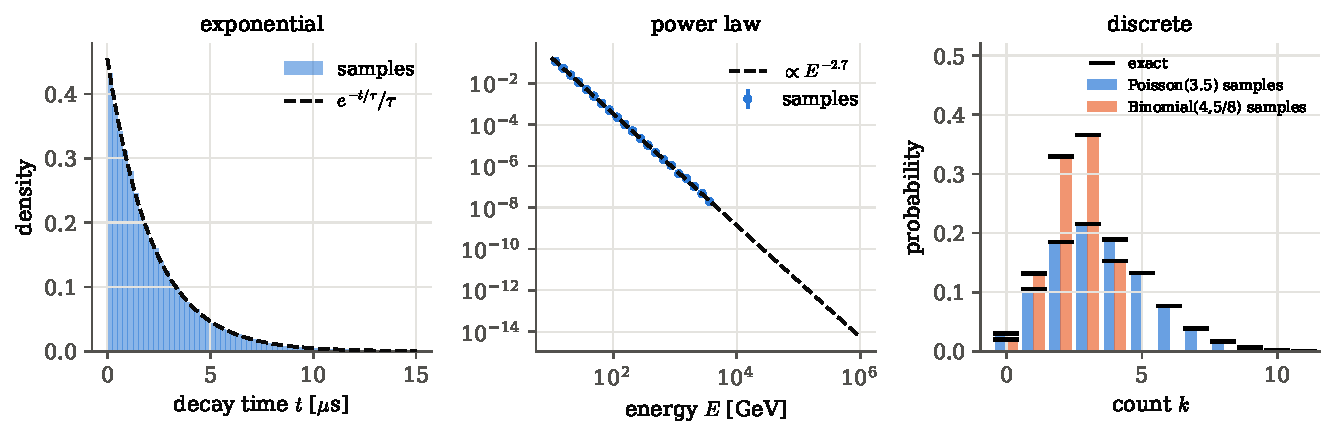
\includegraphics[width=\linewidth]{figures/ch06/inverse_cdf.pdf}
\caption{Samples made by the inverse-CDF method, against the exact
distributions (black dashed). Left: $10^5$ muon decay times. Middle: $10^6$
energies from an $E^{-2.7}$ spectrum between $10\,$GeV and $10^6\,$GeV, on
logarithmic axes, with $\sqrt n$ error bars on bins holding at least ten events; no
simulated energy comes near the upper cut-off. Right: frequencies of Poisson and
binomial counts made by cumulative sums, with the exact probabilities as black
ticks.}
\label{6b:fig:inverse-py}
\end{figure}

\begin{pitfall}[Inverting the wrong thing]
The recipe needs the inverse of the \emph{cumulative} distribution, not of the
density: $x=p^{-1}(u)$ produces nonsense. And a formula for $F$ is not enough: we
must be able to solve $F(x)=u$ for $x$. The Gaussian CDF $\Phi$ has no closed-form
inverse, which is why the next section needs a different trick.
\end{pitfall}

The inverse-CDF method has one more property that the later methods lack: it is
\emph{monotone}. Nearby values of $u$ give nearby values of $x$, and the $x$'s come
out in the same order as the $u$'s. So any structure put into the uniform numbers,
for instance the evenly spread quasi-random points of this chapter's first part or
the strata of \cref{6b:sec:varred}, passes straight through to the target
distribution. Casella and Berger call it a \emph{direct} method: one uniform in,
one draw out, with nothing thrown away \srcref{CasellaBerger}{\S5.6.1}.
\section{Gaussian numbers: Box--Muller and the Cholesky factor}
\label{6b:sec:gauss}

Gaussian noise is everywhere in a simulation. The thermal noise of an amplifier, the
detector noise of a gravitational-wave interferometer, the smearing of a
calorimeter's energy measurement and the primordial fluctuations of the CMB are all
modelled as Gaussian. So we need a fast, exact way to turn uniform numbers into
standard normal numbers $Z\sim\Normal(0,1)$, and then into correlated Gaussian
vectors with any covariance matrix we like.

The inverse-CDF method of \cref{6b:sec:inverse} stalls here, because it needs us to
solve $F(x)=u$ for $x$. The Gaussian CDF,
\[
  \Phi(z)=\frac1{\sqrt{2\pi}}\int_{-\infty}^z e^{-t^2/2}\,\dd t,
\]
has no closed form, and neither does its inverse. A second route also fails.
Sums of logarithms of uniforms build $\chi^2$, gamma and beta variables, for
example
\[
  -2\sum_{j=1}^{\nu}\ln U_j\sim\chi^2_{2\nu},
\]
since each $-2\ln U_j$ is an exponential of mean $2$, which is a $\chi^2_2$
variable. But these sums only produce an \emph{even} number of degrees of freedom.
So they never give $\chi^2_1=Z^2$, and hence never a single normal
\srcref{CasellaBerger}{(5.6.5)}. The way out is to stop asking for one Gaussian and
ask for two.

\subsection{Two Gaussians are easier than one}
\label{6b:sec:boxmuller}

\paragraph{The question.} Which pair of functions of two independent uniforms
$(U_1,U_2)$ gives two independent standard normals $(X,Y)$?

Work backwards from the answer. Two independent standard normals have joint density
\[
  p(x,y)=\frac{1}{\sqrt{2\pi}}e^{-x^2/2}\cdot\frac{1}{\sqrt{2\pi}}e^{-y^2/2}
  =\frac{1}{2\pi}\,e^{-(x^2+y^2)/2}.
\]
This depends only on the distance $r=\sqrt{x^2+y^2}$ from the origin, so it is
rotationally symmetric, like the Maxwell velocity distribution in two dimensions.
A round density is simplest in round coordinates, so switch to polar coordinates
$x=r\cos\theta$, $y=r\sin\theta$. There the area element is
$\dd x\,\dd y=r\,\dd r\,\dd\theta$ (the Jacobian of polar coordinates,
\cref{6b:fig:boxmuller-map}). The probability in a small patch must be the same
whichever coordinates we use to describe it:
\begin{align}
  p_{R,\Theta}(r,\theta)\,\dd r\,\dd\theta
  &\eqby{1}p(x,y)\,\dd x\,\dd y
   \eqby{2}\frac{1}{2\pi}e^{-r^2/2}\,r\,\dd r\,\dd\theta
   \eqby{3}\underbrace{\frac{1}{2\pi}\,\dd\theta}_{\Theta}\;
           \underbrace{r\,e^{-r^2/2}\,\dd r}_{R} .
  \label{6b:eq:polar}
\end{align}
\begin{explain}
  \item Probability is conserved under a change of variables: the patch
        $[r,r+\dd r]\times[\theta,\theta+\dd\theta]$ and its image in the plane
        hold the same probability.
  \item Insert the density, which is $e^{-r^2/2}/2\pi$, and the polar area element
        $r\,\dd r\,\dd\theta$.
  \item The expression is a product of a function of $\theta$ alone and a function
        of $r$ alone, so $R$ and $\Theta$ are independent. $\Theta$ is uniform on
        $[0,2\pi)$ with density $1/2\pi$, and $R$ has density $r\,e^{-r^2/2}$ on
        $r\ge0$ (the Rayleigh distribution of \cref{ch:02}).
\end{explain}
So the problem has split into two easy pieces: make a uniform angle, and make an
independent radius with density $r\,e^{-r^2/2}$.

\emph{The angle.} $\Theta=2\pi U_2$.

\emph{The radius.} It is easier to make its square, $S=R^2$. Since $\dd s=2r\,\dd r$,
the density of $S$ is $p_S(s)\,\dd s=r\,e^{-r^2/2}\dd r=\tfrac12e^{-s/2}\dd s$, an
exponential with mean $2$. (It is $\chi^2_2$, the sum of two squared standard
normals.) An exponential we already know how to make: \eqref{6b:eq:exp} with
$\tau=2$ gives $S=-2\ln U_1$, and $R=\sqrt S$.

Putting the pieces together gives the \newterm{Box--Muller transform}
\cite{BoxMuller1958}, \srcref{CasellaBerger}{Ex.~5.6.4}:
\begin{equation}
  R=\sqrt{-2\ln U_1},\qquad \Theta=2\pi U_2,\qquad
  X=R\cos\Theta,\qquad Y=R\sin\Theta .
  \label{6b:eq:boxmuller}
\end{equation}

We built \eqref{6b:eq:boxmuller} piece by piece, working backwards. Now check it
forwards: start from $(U_1,U_2)$, whose density is $1$ on the unit square, and
compute the density of $(X,Y)$. First invert the map: $U_1=e^{-(X^2+Y^2)/2}$ and
$U_2=\theta(X,Y)/2\pi$, with $\theta$ the polar angle of the point $(X,Y)$. For a
one-to-one change of variables, the new density is the old density times the
absolute value of the Jacobian determinant of the inverse map:
\begin{align}
  p(x,y)
  &\eqby{1}1\cdot\left|\det\begin{pmatrix}
     \partial u_1/\partial x & \partial u_1/\partial y\\
     \partial u_2/\partial x & \partial u_2/\partial y\end{pmatrix}\right|
   \eqby{2}\left|\det\begin{pmatrix}
     -x\,u_1 & -y\,u_1\\[2pt]
     -\dfrac{y}{2\pi r^2} & \dfrac{x}{2\pi r^2}\end{pmatrix}\right|
   \nonumber\\
  &\eqby{3}\left|-\frac{u_1\,(x^2+y^2)}{2\pi r^2}\right|
   \eqby{4}\frac{1}{2\pi}e^{-(x^2+y^2)/2}
   =\frac{e^{-x^2/2}}{\sqrt{2\pi}}\cdot\frac{e^{-y^2/2}}{\sqrt{2\pi}} .
  \label{6b:eq:bm-check}
\end{align}
\begin{explain}
  \item The multivariate change-of-variables rule of \cref{ch:01}, with input
        density $1$.
  \item Differentiate $u_1=e^{-(x^2+y^2)/2}$, which gives $-x\,u_1$ and $-y\,u_1$. For the angle,
        $\theta=\arctan(y/x)$ has $\partial\theta/\partial x=-y/r^2$ and
        $\partial\theta/\partial y=x/r^2$, and $u_2=\theta/2\pi$.
  \item The determinant is $(-x u_1)(x/2\pi r^2)-(-y u_1)(-y/2\pi r^2)$.
  \item $x^2+y^2=r^2$ cancels, and $u_1=e^{-r^2/2}$.
\end{explain}
The result is the product of two standard normal densities, so $X$ and $Y$ are
independent $\Normal(0,1)$: every pair of uniforms gives two Gaussians, exactly,
with no approximation and nothing thrown away.

\begin{figure}[htbp]
\centering
\begin{tikzpicture}[font=\small]
  \begin{scope}[x=3cm,y=3cm]
    \draw[softgray] (0,0) rectangle (1,1);
    \node[below] at (0.5,0) {$u_1$}; \node[left] at (0,0.5) {$u_2$};
    \node[below] at (0,0) {$0$}; \node[below] at (1,0) {$1$};
    \node[left] at (0,1) {$1$};
    \fill[fibreorange!30] (0.28,0) rectangle (0.40,1);
    \fill[formblue!25] (0,0.10) rectangle (1,0.16);
    \fill[bdryred!55] (0.28,0.10) rectangle (0.40,0.16);
    \node[fibreorange!80!black,anchor=south] at (0.34,1.0) {fixed $u_1$};
    \node[formblue,anchor=west] at (1.02,0.13) {fixed $u_2$};
  \end{scope}
  \begin{scope}[xshift=8.2cm,yshift=1.5cm,x=0.75cm,y=0.75cm]
    \draw[->,softgray] (-2.4,0) -- (2.6,0) node[right,black] {$x$};
    \draw[->,softgray] (0,-2.4) -- (0,2.4) node[above,black] {$y$};
    \fill[fibreorange!30,even odd rule] (0,0) circle (1.596) (0,0) circle (1.354);
    \fill[formblue!25] (0,0) -- (36:2.3) arc (36:57.6:2.3) -- cycle;
    \fill[bdryred!55] (36:1.354) -- (36:1.596) arc (36:57.6:1.596) -- (57.6:1.354) arc (57.6:36:1.354) -- cycle;
    \draw[fibreorange] (0,0) circle (1.469);
    \node[fibreorange!80!black,anchor=north east] at (-135:1.6) {$r=\sqrt{-2\ln u_1}$};
    \node[formblue,anchor=south west] at (47:2.3) {$\theta=2\pi u_2$};
    \draw[bdryred,thin] (47:1.6) -- (2.25,0.95);
    \node[bdryred,anchor=west,align=left] at (2.25,0.95) {area\\$r\,\dd r\,\dd\theta$};
  \end{scope}
\end{tikzpicture}
\caption{The Box--Muller map. A vertical strip of the unit square (fixed $u_1$)
becomes a thin ring of radius $\sqrt{-2\ln u_1}$; a horizontal strip (fixed $u_2$)
becomes a wedge at angle $2\pi u_2$, which reaches every radius (it is cut at the edge of the plot). Their overlap, the small red rectangle, is
carried to the red patch of area $r\,\dd r\,\dd\theta$. Small $u_1$ gives large
radii, but the logarithm makes those rare, which produces the Gaussian tails.}
\label{6b:fig:boxmuller-map}
\end{figure}

\paragraph{Example: checking a hundred thousand pairs.}
The script below applies \eqref{6b:eq:boxmuller} to $N=\SixBBmN$ pairs of uniforms.
If the outputs are independent standard normals, five things should hold, and we
check each against its expected scatter.
\begin{itemize}[itemsep=1pt,leftmargin=1.2em]
  \item Means near $0$: they are $\SixBBmMeanX$ and $\SixBBmMeanY$, with standard
        error $1/\sqrt N\approx0.003$.
  \item Variances near $1$: they are $\SixBBmVarX$ and $\SixBBmVarY$, with
        standard error $\sqrt{2/N}\approx0.0045$.
  \item No correlation: the sample correlation is $\SixBBmCorr$.
  \item $X^2+Y^2$ exponential with mean $2$: its mean is $\SixBBmRsqMean$.
  \item Gaussian tails: the fourth moment $\E[X^4]$ is $\SixBBmKurt$, against $3$
        for a Gaussian.
\end{itemize}
A Kolmogorov--Smirnov test of $X$ against $\Normal(0,1)$ (\cref{ch:04}) gives
$p=\SixBBmKS$. \Cref{6b:fig:boxmuller} shows the input square, the output cloud and
the histograms.

\pyfile[firstline=28,lastline=44,firstnumber=28]{code/ch06/22_box_muller.py}{Box--Muller
and its polar variant}

Line 29 is the radius, line 30 the angle, line 31 the two outputs. Line 34 uses
$1-u$ so that $u_1$ lies in $(0,1]$ and $\ln u_1$ is finite.

\paragraph{Example: the polar method.}
Lines 38--44 implement a variant due to Marsaglia and Bray \cite{MarsagliaBray1964}
that avoids computing a sine and a cosine. Box--Muller needs two things: a uniform
number for the radius, and the cosine and sine of a uniform angle. The polar method
gets both from one random point in the unit disc.

\emph{The recipe.} Draw $(V_1,V_2)$ uniform in the square $[-1,1]^2$, and keep the
pair only if $S=V_1^2+V_2^2<1$, that is, only if the point lies in the unit disc.
A kept point is uniform in the disc.

\emph{Why it works.} Its angle is uniform, so $V_1/\sqrt S$ and $V_2/\sqrt S$ are
the cosine and sine of a uniform angle. Its $S$ is uniform on $(0,1)$, because
the fraction of the disc within radius $\sqrt s$ is $\pi s/\pi=s$; and $S$ is
independent of the angle. So $S$ can play the role of $U_1$, and
$X=V_1\sqrt{-2\ln S/S}$, $Y=V_2\sqrt{-2\ln S/S}$ are again independent normals.

\emph{The price.} Some pairs are thrown away. The kept fraction is the area of the
disc over the area of the square, $\pi/4=0.785$, and the script finds
$\SixBBmPolarAcc$. Throwing candidates away to shape a distribution is the whole
idea of the next section.

\begin{figure}[htbp]
\centering
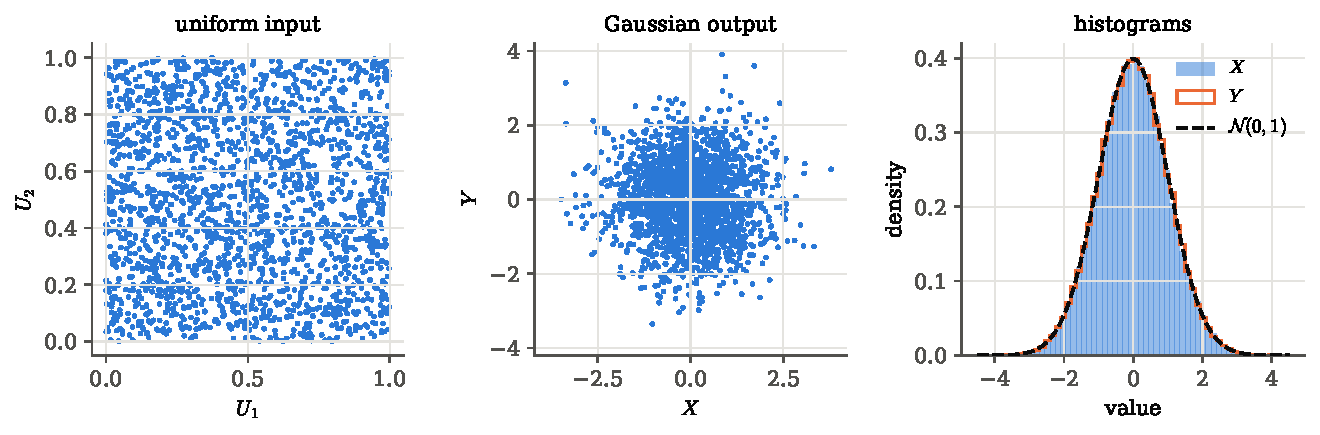
\includegraphics[width=\linewidth]{figures/ch06/box_muller.pdf}
\caption{Box--Muller in action. Left: $2000$ pairs of uniforms. Middle: the same
pairs after the map \eqref{6b:eq:boxmuller}, a round Gaussian cloud. Right: the
histograms of all $10^5$ values of $X$ and of $Y$ lie on the standard normal density
(black dashed).}
\label{6b:fig:boxmuller}
\end{figure}

\begin{pitfall}[Twelve uniforms minus six]
An old shortcut makes a ``Gaussian'' as $U_1+\dots+U_{12}-6$, which has mean $0$
and variance $12\times\tfrac1{12}=1$ and is close to normal by the central limit
theorem (\cref{ch:02}). It can never exceed $6$ in magnitude, and its tails are wrong
long before that. A simulation of the background tail beyond $5\sigma$, which is exactly
where a discovery claim lives, would be wrong. Use an exact method.
\end{pitfall}

\subsection{Correlated Gaussian vectors: the Cholesky factor}
\label{6b:sec:cholesky}

Box--Muller gives independent standard normals. Physics needs correlated ones: the
pixel values of a CMB map, the strain in two detectors driven by a common
environmental noise, the residuals of a fit with a non-diagonal covariance matrix
(\cref{ch:03}). The target is a Gaussian vector $\bm X\sim\Normal(\bm\mu,\Cmat)$ of
dimension $n$ with a prescribed mean vector $\bm\mu$ and covariance matrix $\Cmat$.

\paragraph{The question.} Which linear map turns a vector $\bm z$ of $n$ independent
standard normals, whose covariance is the identity $\Id$, into a vector with
covariance $\Cmat$?

Try $\bm X=\bm\mu+\mathbf L\bm z$ for some $n\times n$ matrix $\mathbf L$. The
transformation rule for covariance matrices under a linear map,
$\Cov(\mathbf A\bm z)=\mathbf A\Cov(\bm z)\mathbf A\T$ (\cref{ch:01}), gives
\begin{align}
  \Cov(\bm X)
  \eqby{1}\Cov(\mathbf L\bm z)
  \eqby{2}\mathbf L\,\Cov(\bm z)\,\mathbf L\T
  \eqby{3}\mathbf L\,\Id\,\mathbf L\T
  =\mathbf L\mathbf L\T .
  \label{6b:eq:cholcov}
\end{align}
\begin{explain}
  \item Adding the constant $\bm\mu$ shifts the vector but not its fluctuations.
  \item The covariance of a linear transformation: $\E[(\mathbf L\bm z)(\mathbf
        L\bm z)\T]=\mathbf L\,\E[\bm z\bm z\T]\,\mathbf L\T$, since $\bm z$ has mean
        zero.
  \item The components of $\bm z$ are independent with unit variance.
\end{explain}
So any $\mathbf L$ with $\mathbf L\mathbf L\T=\Cmat$ gives the right covariance.
The result is also Gaussian, because a linear combination of Gaussians is Gaussian
(\cref{ch:02}). For a
symmetric positive definite $\Cmat$ there is exactly one lower-triangular such
$\mathbf L$ with positive diagonal, the \newterm{Cholesky factor} \unpack{a
``square root'' of $\Cmat$ with zeros above the diagonal}. It costs about $n^3/3$
operations to compute.

\paragraph{Example: two correlated variables.}
For $n=2$ with standard deviations $\sigma_x,\sigma_y$ and correlation coefficient
$\rho$, write $\mathbf L=\bigl(\begin{smallmatrix}l_{11}&0\\l_{21}&l_{22}\end{smallmatrix}\bigr)$
and match $\mathbf L\mathbf L\T$ to $\Cmat$ entry by entry:
\begin{align}
  \begin{pmatrix}l_{11}^2 & l_{11}l_{21}\\ l_{11}l_{21} & l_{21}^2+l_{22}^2\end{pmatrix}
  \eqby{1}\begin{pmatrix}\sigma_x^2 & \rho\sigma_x\sigma_y\\ \rho\sigma_x\sigma_y & \sigma_y^2\end{pmatrix}
  \;\Longrightarrow\;
  l_{11}\eqby{2}\sigma_x,\quad l_{21}\eqby{3}\rho\sigma_y,\quad l_{22}\eqby{4}\sigma_y\sqrt{1-\rho^2}.
  \label{6b:eq:chol2}
\end{align}
\begin{explain}
  \item Multiply out $\mathbf L\mathbf L\T$ and require it to equal the $2\times2$
        covariance matrix.
  \item The top-left entry, taking the positive root.
  \item The off-diagonal entry, divided by $l_{11}=\sigma_x$.
  \item The bottom-right entry: $l_{22}^2=\sigma_y^2-\rho^2\sigma_y^2$.
\end{explain}
So $x=\mu_x+\sigma_xz_1$ and $y=\mu_y+\rho\sigma_yz_1+\sigma_y\sqrt{1-\rho^2}\,z_2$.
In words: $y$ copies a fraction $\rho$ of the fluctuation $z_1$ of $x$, in units of
its own width $\sigma_y$, and adds fresh noise $z_2$ of its own (the same example as
\cref{ch:02}). For $\sigma_x=1$,
$\sigma_y=2$, $\rho=0.8$ this gives $l_{21}=\SixBChLa$ and $l_{22}=\SixBChLb$. From
$50\,000$ draws the sample covariances are $\SixBChSxx$, $\SixBChSxy$ and $\SixBChSyy$,
against $1$, $1.6$ and $4$, and the sample correlation is $\SixBChRho$.

\paragraph{Example: a correlated field on a line.}
A random field is a random function of position. On a grid of $n$ points it is
simply a random vector of $n$ values. ``Statistically homogeneous'' means that the
covariance of the values at two points depends only on their separation $r$. Take $n=\SixBChN$ points on
$[0,20]$ and the exponential correlation $C(r)=e^{-|r|/\ell}$ with correlation length
$\ell=\SixBChEll$, so $\Cmat_{ij}=e^{-|x_i-x_j|/\ell}$. The script factors this
$200\times200$ matrix and draws $M=\SixBChM$ fields $\bm f=\mathbf L\bm z$.

\pyfile[firstline=39,lastline=45,firstnumber=39]{code/ch06/23_cholesky_field.py}{A
correlated one-dimensional Gaussian field by the Cholesky factor}

Line 41 builds the covariance matrix from the separations of all pairs of points,
line 42 factors it, and line 44 multiplies a whole stack of white-noise vectors by
$\mathbf L\T$ from the right, which is the row-vector form of $\mathbf L\bm z$.

What comes out? The realisations (\cref{6b:fig:cholesky}, left) wander smoothly
over distances of order $\ell$, while the white noise they are made from jumps
from point to point. The correlation function estimated from the realisations
follows $e^{-r/\ell}$: at $r=\ell$ it is $\SixBChCfAtEll$, against $e^{-1}=0.368$.
The sample covariance matrix has $40\,000$ entries. The largest deviation of any of
them from $\Cmat$ is $\SixBChMaxDev$. A single entry has standard error
$\sqrt{2/M}=\SixBChExpDev$, so this is about three standard errors, which is what
the largest of $40\,000$ roughly Gaussian errors should be.

\begin{figure}[htbp]
\centering
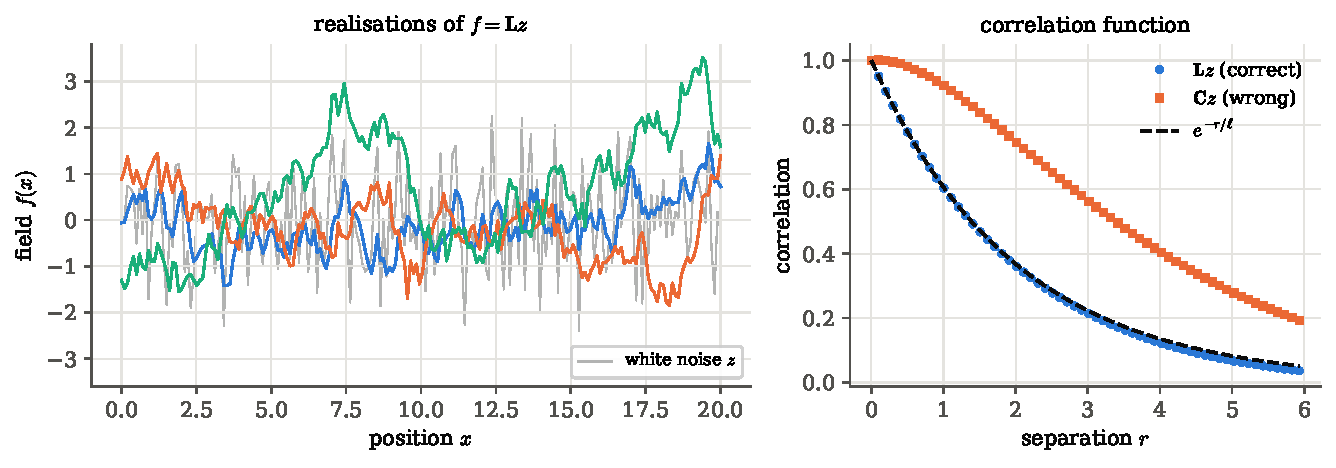
\includegraphics[width=\linewidth]{figures/ch06/cholesky_field.pdf}
\caption{A correlated Gaussian field made from white noise. Left: three realisations
of $\bm f=\mathbf L\bm z$ with correlation length $\ell=2$, and one of the
white-noise vectors $\bm z$ (grey) they are built from. Right: the correlation
function averaged over $4000$ realisations follows $e^{-r/\ell}$ (blue). Multiplying
by $\mathbf C$ instead of its Cholesky factor gives correlations that are far too
long (orange).}
\label{6b:fig:cholesky}
\end{figure}

The orange points of \cref{6b:fig:cholesky} show a tempting mistake: multiplying the
white noise by $\Cmat$ itself. By \eqref{6b:eq:cholcov} with $\mathbf L$ replaced by
$\Cmat$, the result has covariance $\Cmat\Cmat\T=\Cmat^2$, not $\Cmat$; its correlation at
$r=\ell$ is $\SixBChCfBadAtEll$ instead of $0.368$.

\begin{keyidea}[Colouring white noise]
Any Gaussian vector with covariance $\Cmat$ is a linear map of white noise:
$\bm X=\bm\mu+\mathbf L\bm z$ with $\mathbf L\mathbf L\T=\Cmat$ and $\bm z$ a vector of
independent standard normals made by Box--Muller. Conversely,
$\mathbf L^{-1}(\bm X-\bm\mu)$ is white again, which is how correlated residuals are
``whitened'' before a $\chi^2$ is formed.
\end{keyidea}

The Cholesky factor costs $n^3/3$ operations and $n^2$ memory. For a CMB map with
$5\times10^7$ pixels that is hopeless. A statistically isotropic field offers a way
round. Expand it in spherical harmonics; its harmonic coefficients $\alm$ are then
uncorrelated, with variances given by the power spectrum $\Cell$. So in the
harmonic basis the covariance is diagonal, and its ``Cholesky factor'' is simply
$\sqrt{\Cell}$ \unpack{one independent Gaussian per mode, scaled by the square root of
the power spectrum}. Simulating a CMB sky is therefore Box--Muller followed by a
spherical-harmonic transform, which is how \cref{ch:07} and \cref{ch:08} make maps.
Cholesky remains the tool for small, dense covariance matrices: the correlated
residuals of a fit, a few correlated nuisance parameters, or a masked patch of sky.
\section{Rejection sampling: throwing points under a curve}
\label{6b:sec:rejection}

In the reaction $e^+e^-\to\mu^+\mu^-$ at energies well below the $Z$ pole, the
muons come out with the angular distribution
\begin{equation}
  f(x)=\tfrac38\,(1+x^2),\qquad x=\cos\theta\in[-1,1],
  \label{6b:eq:mumu}
\end{equation}
where $\theta$ is the angle between the outgoing $\mu^-$ and the incoming $e^-$
\srcref{Cowan}{(3.8)}. To simulate events we need draws of $x$ from this density.
The inverse-CDF method of \cref{6b:sec:inverse} sets the CDF equal to a uniform
number $u$ and solves for $x$. Here that means solving the cubic
$F(x)=\tfrac18(x^3+3x+4)=u$ for every event. That can still be done. Add the
forward--backward asymmetry, or multiply by a detector efficiency, and the CDF can
no longer be inverted by hand. The posterior densities of \cref{ch:05} are worse
still: we can compute their value at any point, but we know nothing about their
CDF. So we need a method that uses only the \emph{values} of $f$.

\paragraph{The question.} If all we can do is evaluate $f(x)$, and draw from some
simpler density $g$, how do we produce draws from $f$?

\subsection{Points uniform under a curve}
\label{6b:sec:under-curve}

The key fact is geometric. Draw the graph of a density $f$ and consider the region
under it, $A_f=\{(x,y):0<y<f(x)\}$. Its area is $\int f\,\dd x=1$. Now pick a point
$(X,Y)$ uniformly in that region, so its joint density is $1$ on $A_f$ and $0$
elsewhere. The density of its horizontal coordinate alone is the marginal
(\cref{ch:01}), obtained by integrating out the vertical coordinate:
\begin{align}
  p_X(x)\eqby{1}\int p_{X,Y}(x,y)\,\dd y
        \eqby{2}\int_0^{f(x)}1\,\dd y
        \eqby{3}f(x) .
  \label{6b:eq:undercurve}
\end{align}
\begin{explain}
  \item The marginal density of $X$ averages out the nuisance coordinate $Y$.
  \item The joint density is $1$ for $0<y<f(x)$ and zero otherwise.
  \item The length of the vertical slice of $A_f$ at $x$ is the height of the curve.
\end{explain}
So \emph{the $x$-coordinates of points spread uniformly under the graph of $f$ are
draws from $f$}. In words: a tall part of the curve holds more of the points, in
proportion to its height. The same holds if we only know $f$ up to a constant
factor $c>0$. The region under $cf$ has area $c$, so a uniform point in it has
joint density $1/c$, and the $x$-marginal is $cf(x)/c=f(x)$ again. So we never
need the normalising constant of $f$.

How do we get points uniform under $f$? Doing it directly is as hard as drawing
from $f$ itself. Instead, we make points uniform under a \emph{larger} curve that we
know how to sample, and keep only those that happen to fall under $f$. The kept points cover
the region under $f$ evenly, because every part of it was covered evenly before we
threw anything away. So they are uniform under $f$. This is von Neumann's
acceptance--rejection method \srcref{Cowan}{\S3.3}.

\subsection{The algorithm and why it works}
\label{6b:sec:reject-proof}

Choose an \newterm{envelope} density $g$ \unpack{a density we can already sample, for
instance by the inverse CDF} and a constant $M$ with $f(x)\le M g(x)$ for every $x$.
Then repeat:
\begin{enumerate}[itemsep=1pt,leftmargin=1.6em]
  \item draw a candidate $V\sim g$ and, independently, $U\sim\mathrm{Uniform}(0,1)$;
  \item if $U<f(V)/\bigl(M g(V)\bigr)$, accept and return $V$; otherwise reject and go
        back to step 1.
\end{enumerate}
In the picture of points under a curve (\cref{6b:sec:under-curve}), step 1 puts the
point $(V,\,U\,Mg(V))$ uniformly under the curve $Mg$: its horizontal position $V$
has density $g$, and its height $U\,Mg(V)$ is uniform between $0$ and $Mg(V)$.
Step 2 keeps the point if it also lies under $f$, because $U\,Mg(V)<f(V)$ is the
same condition as $U<f(V)/Mg(V)$.

\emph{The question.} Why are the kept values exact draws from $f$, and not
something only close to it? A kept value is a candidate $V$ for which the event
``accept'' happened. So what we need is the CDF of $V$ given acceptance,
$\Prob(V\le y\given\text{accept})$. By the definition of conditional probability
this is $\Prob(V\le y,\ \text{accept})/\Prob(\text{accept})$, so we need two
probabilities \srcref{CasellaBerger}{Thm~5.6.8}.

\emph{First, how often is a candidate accepted?}
\begin{align}
  \Prob(\text{accept})
  &\eqby{1}\int g(v)\,\Prob\Bigl(U<\frac{f(v)}{Mg(v)}\Bigr)\,\dd v
   \eqby{2}\int g(v)\,\frac{f(v)}{Mg(v)}\,\dd v
   \eqby{3}\frac1M\int f(v)\,\dd v
   \eqby{4}\frac1M .
  \label{6b:eq:accept}
\end{align}
\begin{explain}
  \item Law of total probability over the value $v$ of the candidate, which has
        density $g$ (\cref{ch:01}).
  \item $U$ is uniform and $f(v)/Mg(v)\le1$ by the choice of $M$, so the probability
        that $U$ lies below it is the number itself.
  \item The $g$'s cancel.
  \item $f$ is a normalised density.
\end{explain}
\emph{Second, how often is a candidate both accepted and below a value $y$?} It is
the same integral, stopped at $y$. \emph{Then divide}, which gives the CDF we want:
\begin{align}
  \Prob(V\le y,\ \text{accept})
  \eqby{1}\int_{-\infty}^{y}g(v)\,\frac{f(v)}{Mg(v)}\,\dd v
  \eqby{2}\frac{F(y)}{M},
  \qquad
  \Prob(V\le y\given\text{accept})
  \eqby{3}\frac{F(y)/M}{1/M}=F(y) .
  \label{6b:eq:accept-cdf}
\end{align}
\begin{explain}
  \item As in \eqref{6b:eq:accept}, but only candidates below $y$ count.
  \item The $g$'s cancel, and $\int_{-\infty}^y f=F(y)$.
  \item The definition of conditional probability (\cref{ch:01}), with
        \eqref{6b:eq:accept} in the denominator.
\end{explain}
\emph{What it means.} The accepted values have CDF $F$, so they are exact draws
from $f$, with no approximation. In the language of \cref{ch:01}, accepting is
\emph{conditioning}. We generate candidates from a larger sample space and keep only
the outcomes in the event ``the point fell under $f$''. Keeping only that event
turns the distribution $g$ of the candidates into the distribution $f$ of the
survivors.

\begin{figure}[htbp]
\centering
\begin{tikzpicture}[x=2.3cm,y=3.6cm,font=\small]
  \draw[->,softgray] (0,0) -- (4.35,0) node[right,black] {$x$};
  \draw[->,softgray] (0,0) -- (0,1.42);
  \pgfmathsetseed{11}
  \foreach \i in {1,...,230} {
    \pgfmathsetmacro{\vx}{-ln(max(rnd,0.0005))}
    \pgfmathsetmacro{\vy}{rnd*1.3155*exp(-\vx)}
    \pgfmathsetmacro{\fx}{0.7979*exp(-\vx*\vx/2)}
    \ifdim \vx pt < 4.2pt
      \ifdim \vy pt < \fx pt
        \fill[formblue] (\vx,\vy) circle (1.1pt);
      \else
        \fill[fibreorange] (\vx,\vy) circle (1.1pt);
      \fi
    \fi
  }
  \draw[tangentgreen!70!black,thick,domain=0:4.2,samples=100] plot (\x,{1.3155*exp(-\x)});
  \draw[black,thick,domain=0:4.2,samples=100] plot (\x,{0.7979*exp(-\x*\x/2)});
  \node[tangentgreen!70!black,anchor=west] at (0.55,1.05) {envelope $Mg(x)=M e^{-x}$};
  \node[anchor=west] at (1.55,0.40) {target $f(x)=\sqrt{2/\pi}\,e^{-x^2/2}$};
  \draw[softgray] (1.0,0.484) -- (1.53,0.40);
  \node[formblue,anchor=west] at (2.7,1.25) {accepted: under $f$};
  \node[fibreorange,anchor=west] at (2.7,1.12) {rejected: between $f$ and $Mg$};
  \node[below] at (1,0) {$1$}; \node[below] at (2,0) {$2$}; \node[below] at (3,0) {$3$};
\end{tikzpicture}
\caption{Rejection sampling as throwing points under a curve. Each candidate $x$ is
drawn from the exponential density $g$ and given a height uniform between $0$ and
$Mg(x)$ (green), so the points are uniform under the green curve. The points that
fall under the target $f$ (black) are kept; their $x$-coordinates are distributed as
$f$. The fraction kept is the area under $f$ divided by the area under $Mg$, which is
$1/M$. The two curves touch at $x=1$, where $f/g$ is largest.}
\label{6b:fig:reject-geom}
\end{figure}

\emph{The cost.} Each candidate is accepted independently with probability $1/M$,
by \eqref{6b:eq:accept}.
So the number $K$ of candidates needed for one accepted value is geometric,
$\Prob(K=k)=(1-1/M)^{k-1}/M$: $k-1$ rejections followed by one acceptance. Its mean
is $\E K=\sum_k k\,(1-1/M)^{k-1}/M=M$ \srcref{CasellaBerger}{(5.6.12)}. So $M$ is
the average cost of one draw, counted in candidates.

\emph{The best envelope.} Since $M$ is the cost, the best envelope is the one with
the smallest $M$. Two choices achieve that. First, take $M=\sup_x f(x)/g(x)$
exactly: this is the smallest value that still keeps $Mg$ above $f$ everywhere.
Second, choose $g$ as close in shape to $f$ as possible, so that this supremum is
itself close to $1$.

\begin{workdef}[rejection sampling]
Target $f$ (known up to a constant), envelope $g$ that we can sample, and
$M=\sup_x f(x)/g(x)<\infty$ \unpack{the factor that lifts $g$ above $f$ everywhere}.
Draw $V\sim g$, $U\sim\mathrm{Uniform}(0,1)$; keep $V$ if $U\,Mg(V)<f(V)$.
\emph{Cost:} on average $M$ candidates per accepted draw; acceptance rate $1/M$.
\emph{Requirement:} $f/g$ must be bounded, so $g$ needs tails at least as heavy as
$f$'s.
\end{workdef}

\subsection{Three worked examples}
\label{6b:sec:reject-examples}

\paragraph{Example: the muon-pair angle in a box.}
The simplest envelope is a box. For \eqref{6b:eq:mumu} on $[-1,1]$, the largest value of
$f$ is $f_{\max}=f(\pm1)=3/4$. Take $g$ uniform on $[-1,1]$, so $g=1/2$ and
$M=f_{\max}/g=3/2$. The recipe becomes three steps: draw $x$ uniform on $[-1,1]$,
draw $u$ uniform on $[0,f_{\max}]$, and keep $x$ if $u<f(x)$ \srcref{Cowan}{\S3.3}.
The predicted acceptance is $1/M=2/3$: the area under $f$ (one) divided by the
area of the box ($2\times3/4$). Out of $\SixBRjN$ candidates the script accepts a
fraction $\SixBRjMuAcc$. To check the shape as well, compare the mean of $x^2$ over
accepted values, $\SixBRjMuMeanSq$, with its exact value,
$\int_{-1}^1x^2\cdot\frac38(1+x^2)\,\dd x=\frac38\bigl(\frac23+\frac25\bigr)=\frac25$.
\Cref{6b:fig:rejection} (left and middle) reproduces Cowan's Figure 3.2.

\paragraph{Example: a half-normal under an exponential.}
Take $f(x)=\sqrt{2/\pi}\,e^{-x^2/2}$ for $x>0$, the distribution of $|Z|$ for a standard
normal $Z$, and the envelope $g(x)=e^{-x}$, which we sample as $-\ln(1-u)$. The ratio and
its maximum:
\begin{align}
  \frac{f(x)}{g(x)}
  \eqby{1}\sqrt{\frac2\pi}\;e^{\,x-x^2/2}
  \eqby{2}\sqrt{\frac2\pi}\;e^{1/2}\,e^{-(x-1)^2/2}
  \quad\Longrightarrow\quad
  M=\sup_x\frac fg\eqby{3}\sqrt{\frac{2e}{\pi}}=\SixBRjHnM .
  \label{6b:eq:halfnormal}
\end{align}
\begin{explain}
  \item Divide the two densities: $e^{-x^2/2}/e^{-x}=e^{x-x^2/2}$.
  \item Complete the square: $x-\tfrac12x^2=\tfrac12-\tfrac12(x-1)^2$.
  \item The Gaussian factor is at most $1$, reached at $x=1$, where the two curves
        touch (\cref{6b:fig:reject-geom}).
\end{explain}
So a fraction $1/M=\SixBRjHnInvM$ of candidates should survive; the script finds
$\SixBRjHnAcc$. The number of candidates per accepted value averages
$\SixBRjTrialsMean$, against $M$, and its histogram is the geometric distribution
(\cref{6b:fig:rejection-trials}). The accepted values have mean $\SixBRjHnMean$, against
$\E|Z|=\sqrt{2/\pi}=\SixBRjHnExactMean$. Attaching a random sign to each accepted
value gives a full standard normal. That is a third Gaussian generator, after
Box--Muller and the polar method.

\paragraph{Example: a Beta density with non-integer parameters.}
Take $Y\sim\mathrm{Beta}(a,b)$ with $a=2.7$ and $b=6.3$. The recipes of
\cref{6b:sec:gauss} that build gamma and beta variables from logarithms of uniforms
need integer parameters, so they do not apply here, and there is no other simple
transformation from uniforms. Rejection needs none: put the density on
$[0,1]$ inside a box of width $1$ and height $c=\max_yf_Y(y)$
\srcref{CasellaBerger}{Ex.~5.6.7}. Here $g$ is uniform on $[0,1]$, so $M=c$. The
maximum is at the mode $y=(a-1)/(a+b-2)=1.7/7$, where $c=\SixBRjBetaC$. So the
acceptance should be $1/c=\SixBRjBetaInvC$; the script finds $\SixBRjBetaAcc$. The
mean of accepted values is $\SixBRjBetaMean$, against $a/(a+b)=0.3$.

Can a better envelope help? A $\mathrm{Beta}(2,6)$ envelope is closer in shape
to the target, and needs only $M=1.67$ candidates per draw instead of $2.67$. But each
$\mathrm{Beta}(2,6)$ candidate itself costs several uniforms. So which algorithm is
faster depends on the cost of a candidate as well as on $M$
\srcref{CasellaBerger}{Ex.~5.6.9}.

\begin{figure}[htbp]
\centering
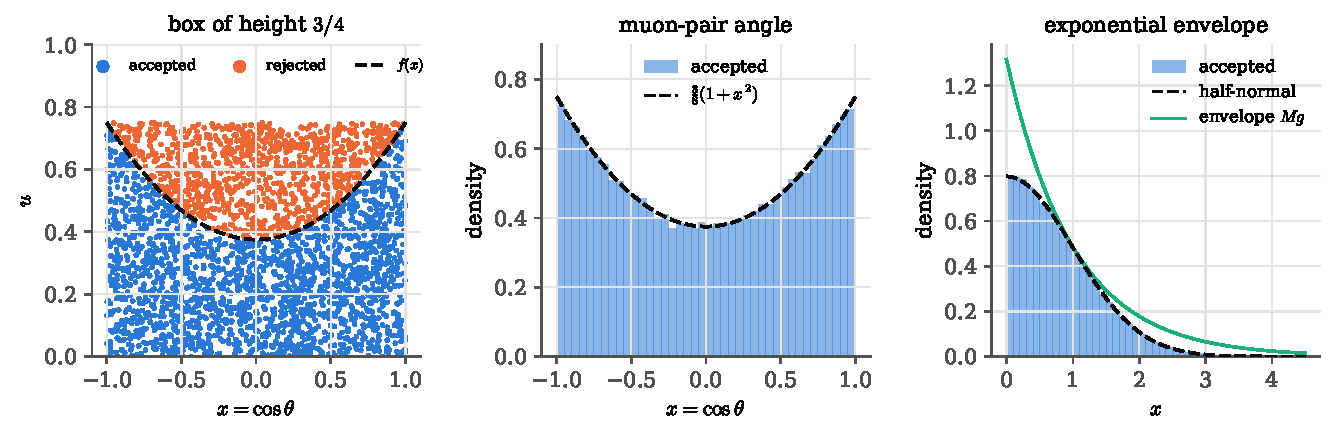
\includegraphics[width=\linewidth]{figures/ch06/rejection.pdf}
\caption{Rejection sampling at work. Left: $3000$ candidate points uniform in the box
of height $3/4$; those under $f(x)=\tfrac38(1+x^2)$ (blue) are kept. Middle: the
histogram of all kept $x=\cos\theta$ values follows the muon-pair angular distribution.
Right: half-normal values kept from exponential candidates, with the envelope $Mg$
(green) touching the target at $x=1$.}
\label{6b:fig:rejection}
\end{figure}

\pyfile[firstline=39,lastline=45,firstnumber=39]{code/ch06/24_rejection.py}{Half-normal
draws from exponential candidates}

Line 41 draws the candidates by the inverse CDF of \cref{6b:sec:inverse}, line 43
computes the acceptance probability $f(V)/Mg(V)$ for all of them at once, and line 44 keeps
the candidates whose uniform number falls below it. The loop ``repeat until accepted'' of
the algorithm has become a filter applied to a fixed number of candidates at once.
This is how rejection is usually coded in numpy. The price is that $N$ candidates
give about $N/M$ accepted values, not exactly $N$.

\begin{figure}[htbp]
\centering
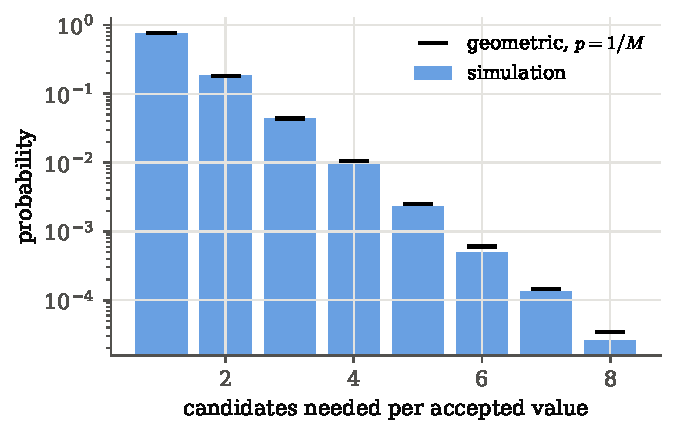
\includegraphics[width=0.55\linewidth]{figures/ch06/rejection_trials.pdf}
\caption{How many exponential candidates it takes to get one half-normal value. The
frequencies (bars, logarithmic scale) fall by a factor $1-1/M$ per extra candidate,
the geometric distribution with success probability $1/M$ (black ticks).}
\label{6b:fig:rejection-trials}
\end{figure}

\subsection{When rejection fails: tails and dimension}
\label{6b:sec:reject-limits}

Rejection fails in two ways. The first is in the tails. The method needs a finite
$M=\sup f/g$, so that $Mg$ lies above $f$ everywhere. If the target has heavier tails
than the envelope, then far out $f$ is much larger than $g$, the ratio $f/g$ grows
without bound, and no finite $M$ exists. A Cauchy envelope for a Gaussian
target works, since the Cauchy tails, falling as $x^{-2}$, outlast $e^{-x^2/2}$. A
Gaussian envelope for a Cauchy target cannot work, however large we make $M$
\srcref{CasellaBerger}{p.~207}. The same condition on the tails comes back, in a sharper
form, for importance sampling in \cref{6b:sec:importance}.

The second failure is in high dimension, and it is worse because nothing visibly
breaks: the acceptance rate just collapses. In $d$ dimensions the envelope has to
cover the target in every direction at once, and the wasted volume multiplies. The cleanest example
is the uniform distribution in the unit ball, sampled from the cube $[-1,1]^d$ around it.
The acceptance is the volume of the ball over the volume of the cube:
\begin{align}
  \frac1M
  &\eqby{1}\frac{\pi^{d/2}/\Gamma(d/2+1)}{2^d},
  \qquad\text{so}\qquad \frac1M=\frac{\pi}{4}=0.785\ \text{ for } d=2, \nonumber\\
  \frac1M&\eqby{2}\frac{\pi^5}{5!\;2^{10}}=0.0025\ \text{ for } d=10,\qquad
  \frac1M\eqby{3}\frac{\pi^{10}}{10!\;2^{20}}=2.5\times10^{-8}\ \text{ for } d=20 .
  \label{6b:eq:ball}
\end{align}
\begin{explain}
  \item The volume of the unit ball in $d$ dimensions is $\pi^{d/2}/\Gamma(d/2+1)$;
        the cube of side $2$ has volume $2^d$.
  \item $\Gamma(6)=5!=120$, so $306.0/(120\times1024)$.
  \item $\Gamma(11)=10!=3\,628\,800$, and $\pi^{10}=93\,648$.
\end{explain}
In two dimensions (the polar method of \cref{6b:sec:boxmuller}) we keep $79\%$ of the
candidates. In twenty dimensions we keep one candidate in forty million. A
cosmological posterior with twenty parameters is far more concentrated inside its
prior than a ball is inside a cube, so rejection from the prior is hopeless there.
This is the practical reason for the Markov chain methods of \cref{ch:09}, which
never try to cover the whole space at once.

Rejection also hides inside some recipes that do not use the word. In a
dose--response study, ten response probabilities $p_1,\dots,p_{10}$, one per dose,
each have an independent Beta posterior, but physics says they must be ordered,
$p_1\le\dots\le p_{10}$. The recipe is: draw all ten, and throw the draw away if it
is not ordered \mainref{Ex.~24.4, p.~407}. That is rejection sampling. By exactly
the argument of \eqref{6b:eq:accept-cdf}, the kept draws come from the posterior
restricted to the ordered region, and the acceptance rate is the posterior
probability of that region.

\begin{keyidea}[Accepting is conditioning]
Points uniform under the graph of a density have $x$-coordinates distributed as that
density. Rejection sampling makes points uniform under an easy envelope $Mg$ and keeps
those under $f$; the survivors are exact draws from $f$, at an average cost of $M$
candidates each. It needs only values of $f$ up to a constant, and it breaks down when
$f/g$ is unbounded or when the dimension is large.
\end{keyidea}
\section{Monte Carlo integration and the $1/\sqrt N$ law}
\label{6b:sec:mcint}

Almost every number we want out of a probability model is an integral. The
posterior mean of a parameter is $\int\theta\,p(\theta\given\data)\,\dd\theta$. The
marginal posterior of one cosmological parameter is an integral over the other five.
The normalising constant of Bayes' theorem, the evidence, is an integral of likelihood
times prior over the whole parameter space \mainref{\S24.1, p.~403},
\srcref{Lambert}{\S12.3}. The acceptance of a detector is an integral of the emission
density over the directions that hit it. Most of these integrals have no closed form.
Even a one-parameter model with a Poisson likelihood and a log-normal prior gives one,
and each added parameter makes it harder \srcref{Lambert}{\S12.3}. Grids and
quadrature rules work in one or two dimensions. Beyond that the number of grid
points, $n^D$ for $n$ points per axis in $D$ dimensions, becomes too large to evaluate
\srcref{Lambert}{\S12.4--12.5}.

The samplers built so far (the inverse CDF, Box--Muller and rejection) give another
way, resting on two facts: an average over random draws estimates an expectation, and
every integral can be written as an expectation. Lambert tells the first fact as a
story about a box with a die inside. We cannot see the die, but we can shake the box and
read the face through a small window. The average of many readings estimates the
mean of the die, without our knowing how many faces it has or how it is loaded
\srcref{Lambert}{\S12.6}.

\paragraph{The question.} If we estimate an integral by averaging a function over $N$
random draws, how large is the error, and how does it depend on $N$ and on the dimension?

\subsection{An integral is an expectation}
\label{6b:sec:int-expect}

Start with a one-dimensional integral $I=\int_a^bh(x)\,\dd x$. Multiply and divide by
$b-a$ \mainref{(24.1)}:
\begin{align}
  I
  \eqby{1}\int_a^b\underbrace{h(x)\,(b-a)}_{w(x)}\;\underbrace{\frac{1}{b-a}}_{f(x)}\,\dd x
  \eqby{2}\E_f\bigl[w(X)\bigr],\qquad X\sim\mathrm{Uniform}(a,b) .
  \label{6b:eq:int-expect}
\end{align}
\begin{explain}
  \item Nothing has changed: we multiplied and divided by the same constant.
  \item $f(x)=1/(b-a)$ is the uniform density on $[a,b]$, and an integral of a function
        against a density is the expectation of that function.
\end{explain}
More generally, any integral of the form $I=\int h(x)f(x)\,\dd x$ with $f$ a density is
$\E_f[h(X)]$ \mainref{(24.3)}, and the variable $x$ can have any number of dimensions.
Draw $X_1,\dots,X_N$ independently from $f$ and average:
\begin{equation}
  \hat I=\frac1N\sum_{i=1}^Nh(X_i) .
  \label{6b:eq:mc-estimator}
\end{equation}
By the law of large numbers (\cref{ch:03}), $\hat I\to I$ as $N\to\infty$
\mainref{(24.2)}, \srcref{CasellaBerger}{(5.6.4)}.

\begin{workdef}[Monte Carlo estimate of an integral]
Write the integral as an expectation, $I=\E_f[h(X)]$ \unpack{choose a density $f$ we can
sample, and put everything else into $h$}. Draw $N$ independent $X_i\sim f$ and report
\[
  \hat I=\frac1N\sum_ih(X_i)\ \pm\ \frac{s}{\sqrt N},\qquad
  s^2=\frac{1}{N-1}\sum_i\bigl(h(X_i)-\hat I\bigr)^2 .
\]
The error bar is itself estimated from the same draws.
\end{workdef}

\subsection{Why the error falls as $1/\sqrt N$}
\label{6b:sec:sqrtN}

The estimator $\hat I$ of \eqref{6b:eq:mc-estimator} is an average of $N$
independent terms $h(X_i)$. How far is it from $I$? Call $\mu=\E_f[h(X)]=I$ and
$\sigma^2=\Var_f[h(X)]$ the mean and variance of a single term. The mean and the
variance of the average then follow in two lines each:
\begin{align}
  \E[\hat I]&\eqby{1}\frac1N\sum_{i=1}^N\E[h(X_i)]\eqby{2}I,\nonumber\\
  \Var[\hat I]&\eqby{3}\frac1{N^2}\sum_{i=1}^N\Var[h(X_i)]
               \eqby{4}\frac{N\sigma^2}{N^2}=\frac{\sigma^2}{N} .
  \label{6b:eq:mc-var}
\end{align}
\begin{explain}
  \item Expectation is linear.
  \item Each $X_i$ has density $f$, so each term has mean $I$.
  \item The $X_i$ are independent, so the variance of the sum is the sum of the
        variances, and a constant factor $1/N$ comes out squared.
  \item Each term has variance $\sigma^2$.
\end{explain}
So $\hat I$ is unbiased, and its standard error, the square root of its variance, is
$\sigma/\sqrt N$. This is the same law that made the error of a sample mean shrink in
\cref{ch:03}. The central limit theorem (\cref{ch:02}) adds the shape: for large $N$,
$\hat I$ is approximately Gaussian, $\hat I\approx\Normal(I,\sigma^2/N)$. We do not know
$\sigma$, so we replace it by $s$, the standard deviation of the $N$ values $h(X_i)$,
$s^2=\frac{1}{N-1}\sum_i\bigl(h(X_i)-\hat I\bigr)^2$. Then $\hat I\pm1.96\,s/\sqrt N$ is an approximate
$95\%$ confidence interval: in $95\%$ of repeated Monte Carlo runs it covers the true
$I$ \mainref{p.~405}. The CLT needs $\sigma^2<\infty$; \cref{6b:sec:importance} shows
what happens when it is not.

Two facts about $\sigma/\sqrt N$ matter most. First, the factor $1/\sqrt N$ is
slow: to gain one decimal digit we need a hundred times more draws. Second, nothing in
\eqref{6b:eq:mc-var} refers to the dimension of $x$. A thousand-dimensional integral has
error $\sigma/\sqrt N$ exactly like a one-dimensional one; only $\sigma$ can depend on the
problem.

\begin{keyidea}[The Monte Carlo error law]
The average of $h$ over $N$ independent draws from $f$ estimates $\int hf$ with standard
error $\sigma/\sqrt N$, where $\sigma^2=\Var_f[h]$. The rate $N^{-1/2}$ does not depend
on the dimension; the constant $\sigma$ does depend on how well $f$ matches where $h$ is
large, and every variance-reduction method works on $\sigma$.
\end{keyidea}

\paragraph{Example: $\int_0^1x^3\,\dd x$.}
Here $f$ is uniform on $[0,1]$ and $h(x)=x^3$, so $I=1/4$ and
$\sigma^2=\E[U^6]-(\E[U^3])^2=\tfrac17-\tfrac1{16}=\tfrac{9}{112}$, that is
$\sigma=\SixBMcCubeSig$. With $N=\SixBMcCubeN$ uniforms the script finds
$\hat I=\SixBMcCube\pm\SixBMcCubeSe$, where the error bar is $s/\sqrt N$; the prediction
is $\sigma/\sqrt N=0.0028$, and Wasserman reports $0.248\pm0.0028$
\mainref{Ex.~24.1}. To see the law itself, the script repeats the estimate $2000$ times at
each of thirteen values of $N$ from $10$ to $10^5$ and measures the root-mean-square
error. On a log--log plot the points fall on a line of slope $\SixBMcSlope$
(\cref{6b:fig:mc-error}, left), and at $N=10^5$ the measured RMS error is $\SixBMcRmsRatio$
times $\sigma/\sqrt N$.

\paragraph{Example: a probability is the mean of an indicator.}
To compute $\Phi(2)=\Prob(Z\le2)$ for $Z\sim\Normal(0,1)$, write it as
$\int h(s)\,\varphi(s)\,\dd s$ with $\varphi$ the standard normal density and $h(s)=1$ if $s\le2$,
$0$ otherwise \mainref{Ex.~24.2}. The Monte Carlo estimate is then the fraction of
normal draws below $2$. Each term is a Bernoulli variable with $\sigma^2=p(1-p)$, so the
standard error is the binomial $\sqrt{p(1-p)/N}$. The script gives $\SixBMcPhiFour\pm\SixBMcPhiSeFour$
for $N=10^4$ and $\SixBMcPhiFive\pm\SixBMcPhiSeFive$ for $N=10^5$, against $\SixBMcPhiExact$.
Every probability of an event can be computed this way: simulate the experiment and count.
Casella and Berger's example asks for the probability that at least $t$ of $c$ electronic
components with exponential lifetimes survive $h$ hours; the Monte Carlo answer is the
fraction of simulated batches in which they do \srcref{CasellaBerger}{Ex.~5.6.2}.

\subsection{Grids lose in high dimension}
\label{6b:sec:grid-vs-mc}

A grid rule beats $1/\sqrt N$ easily in one dimension, and loses that advantage as the
dimension grows. Take the midpoint rule with spacing $\Delta$: it replaces $h$ on each cell
by its value at the cell's midpoint. For a smooth integrand its error is of order
$\Delta^2$. Why? Expand $h$ in a Taylor series about the midpoint. The linear term is odd
about the midpoint, so it integrates to zero over the cell, and the first term that
survives is quadratic. Now spend $N$ points in $d$ dimensions. A grid gives only
$n=N^{1/d}$ points per axis, so
\begin{align}
  \text{grid error}\;\propto\;\Delta^2\eqby{1}\Bigl(\frac{1}{n}\Bigr)^{2}\eqby{2}N^{-2/d},
  \qquad
  \text{Monte Carlo error}\;=\;\sigma\,N^{-1/2} .
  \label{6b:eq:grid-vs-mc}
\end{align}
\begin{explain}
  \item On the unit cube the spacing is $\Delta=1/n$.
  \item $N=n^d$ points on a grid with $n$ points per axis.
\end{explain}
The two rates are equal when $2/d=1/2$, at $d=4$. Below four dimensions the grid wins;
above it Monte Carlo wins, and by a margin that grows with $d$ \srcref{Cowan}{\S3.4}.
(Gaussian quadrature or Simpson's rule raise the power $2$, which moves the crossover but
not the conclusion; the grid still needs $n^d$ points.)

\paragraph{Example: the same integral in 1, 2, 4 and 8 dimensions.}
On the unit cube take the product
\[
  h(\bm x)=\prod_{i=1}^d\tfrac\pi2\sin(\pi x_i).
\]
Each factor integrates to one, so $I_d=1$ in every dimension. For Monte Carlo with uniform
draws,
\begin{align}
  \sigma_d^2\eqby{1}\E[h^2]-I_d^2
  \eqby{2}\prod_{i=1}^d\E\Bigl[\tfrac{\pi^2}{4}\sin^2(\pi U_i)\Bigr]-1
  \eqby{3}\Bigl(\frac{\pi^2}{8}\Bigr)^{d}-1 .
  \label{6b:eq:sigma-d}
\end{align}
\begin{explain}
  \item The variance is the mean square minus the square of the mean.
  \item The coordinates are independent, so the expectation of the product is the product
        of the expectations.
  \item $\E[\sin^2(\pi U)]=\tfrac12$ for $U$ uniform on $[0,1]$.
\end{explain}
So $\sigma_1=\SixBMcSigOne$ and $\sigma_8=\SixBMcSigEight$. \Cref{6b:fig:mc-error} (right)
compares the two methods for the same number of function evaluations. With about $10^6$
points, the grid error is $\SixBMcGridErrOne$ in one dimension, $\SixBMcGridErrTwo$ in two,
$\SixBMcGridErrFour$ in four ($\SixBMcNptsFour$ points) and $\SixBMcGridErrEight$ in eight
($6^8=\SixBMcNptsEight$ points), while the Monte Carlo errors are $\SixBMcMcErrOne$,
$\SixBMcMcErrTwo$, $\SixBMcMcErrFour$ and $\SixBMcMcErrEight$. In eight dimensions a grid of
$1.7$ million points has only six points per axis, and it is sixty times worse than the
same number of random points.

\begin{figure}[htbp]
\centering
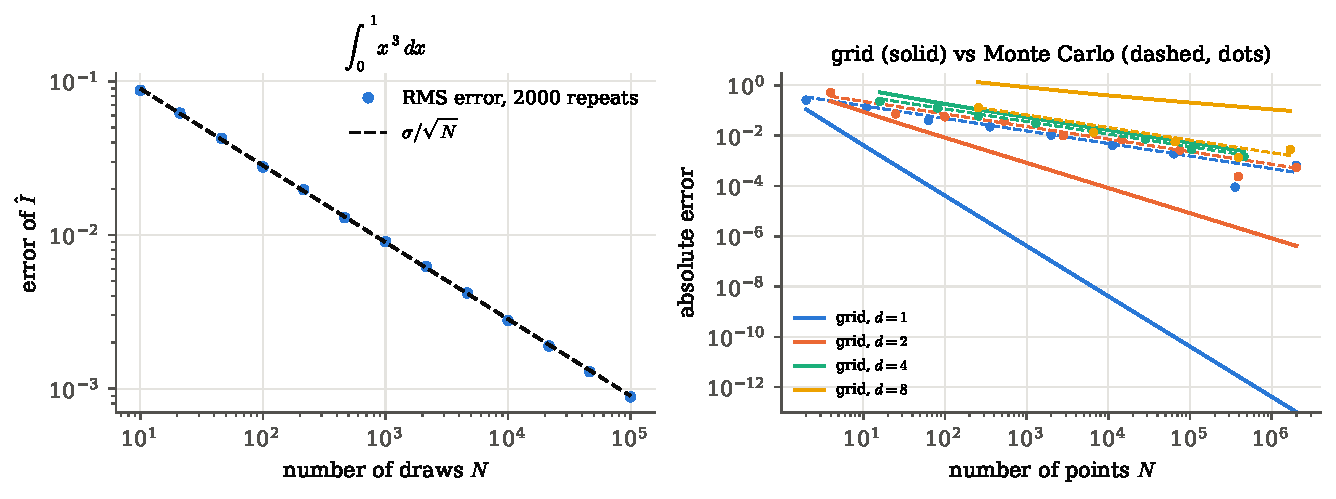
\includegraphics[width=\linewidth]{figures/ch06/mc_error.pdf}
\caption{The $1/\sqrt N$ law. Left: RMS error of the Monte Carlo estimate of
$\int_0^1x^3\dd x$ over $2000$ repeats, against $\sigma/\sqrt N$ (black dashed). Right: the
error for $\int\prod\tfrac\pi2\sin(\pi x_i)\,\dd^dx=1$ with $N$ points. Solid lines: midpoint
grid, error $\propto N^{-2/d}$. Dashed lines and dots: Monte Carlo, error
$\sigma_d/\sqrt N$ with slope $-1/2$ in every dimension. The grid wins for $d=1,2$, roughly
ties at $d=4$ and loses badly at $d=8$.}
\label{6b:fig:mc-error}
\end{figure}

\begin{pitfall}[Dimension-independent is not dimension-free]
The \emph{rate} $N^{-1/2}$ does not depend on $d$, but $\sigma_d$ can grow exponentially
with $d$, as \eqref{6b:eq:sigma-d} shows: $(\pi^2/8)^{d/2}$. It grows much faster when the
integrand is concentrated in a small part of the region we sample. The evidence estimated by
averaging the likelihood over prior draws was exactly that failure (\cref{ch:05}). Monte
Carlo beats the curse of dimensionality only when the sampling density $f$ follows the
integrand, which is what importance sampling and MCMC are for.
\end{pitfall}

\paragraph{Example: a posterior by simulation.}
Integrals over posteriors are where Monte Carlo pays most. Suppose
$X\sim\mathrm{Binomial}(n,p_1)$ and $Y\sim\mathrm{Binomial}(m,p_2)$ are the numbers of
events passing a selection cut in two runs, out of $n$ and $m$ events. We want the
difference of the two efficiencies, $\delta=p_2-p_1$ \mainref{Ex.~24.3}. With flat priors
the posterior factorises into $p_1\given X\sim\mathrm{Beta}(X+1,n-X+1)$ and
$p_2\given Y\sim\mathrm{Beta}(Y+1,m-Y+1)$ (\cref{ch:05}). So we can draw $(p_1,p_2)$ pairs
exactly, form $\delta=p_2-p_1$ for each pair, and make a histogram. The posterior of
$\delta$ is a double integral, and we never have to write it down.

For $n=m=10$, $X=8$, $Y=6$, $\SixBMcDeltaN$ draws give:
\begin{itemize}[itemsep=1pt,leftmargin=1.2em]
  \item a posterior mean $\SixBMcDeltaMean\pm\SixBMcDeltaSe$ (exact:
        $\tfrac7{12}-\tfrac9{12}=-\tfrac16$);
  \item a $95\%$ posterior interval $[\SixBMcDeltaLo,\,\SixBMcDeltaHi]$, from the $2.5\%$
        and $97.5\%$ quantiles of the draws (Wasserman: $(-0.52,0.20)$ from $1000$ draws);
  \item a posterior probability $\Prob(\delta<0\given\data)=\SixBMcDeltaPneg$ that the
        second run has the lower efficiency (\cref{6b:fig:two-binomials}).
\end{itemize}
Each of these is a summary of the draws standing in for the same summary of the
posterior. A quantile of the draws estimates a quantile of the posterior. The fraction of
draws in a region estimates the probability of the region. The histogram estimates the
density, which is the subject of \cref{6b:sec:histogram}.

\begin{figure}[htbp]
\centering
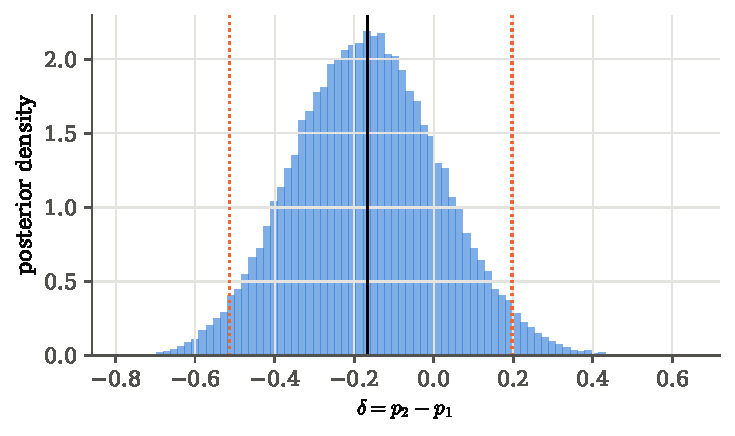
\includegraphics[width=0.55\linewidth]{figures/ch06/mc_two_binomials.pdf}
\caption{Posterior of the difference $\delta=p_2-p_1$ of two binomial probabilities, from
$10^5$ pairs of Beta draws. The solid line is the posterior mean, the dotted lines the
$2.5\%$ and $97.5\%$ quantiles of the draws.}
\label{6b:fig:two-binomials}
\end{figure}

\subsection{Example: the acceptance of a detector}
\label{6b:sec:acceptance}

A radioactive source sits at distance $d$ in front of a flat square scintillator of side
$a$, centred on the axis. It emits isotropically, that is, equally in all directions. What fraction of the decays
hits the scintillator? The answer is the \newterm{geometric acceptance}
$\epsilon=\Omega/4\pi$ \unpack{the solid angle subtended by the detector as a fraction of
the full sphere}. In the Monte Carlo form it is the mean of an indicator: emit $N$
particles in isotropic directions (\cref{6b:sec:inverse-cont}: $\cos\theta=2u_1-1$,
$\phi=2\pi u_2$), follow each straight line to the plane $z=d$, and count the fraction that
lands inside the square.

\begin{figure}[htbp]
\centering
\begin{tikzpicture}[font=\small,x=1cm,y=1cm]
  \fill[formblue!15] (4,-2) rectangle (4.25,2);
  \draw[formblue,thick] (4,-2) -- (4,2);
  \fill (0,0) circle (2pt);
  \node[anchor=east] at (-0.1,0) {source};
  \draw[softgray,dashed] (0,0) -- (6,0);
  \foreach \ang in {-24,-12,5,17} \draw[tangentgreen,->] (0,0) -- ({4/cos(\ang)*cos(\ang)},{4*tan(\ang)});
  \foreach \ang in {40,-45,150,-120} \draw[fibreorange,->] (0,0) -- (\ang:2.6);
  \draw[softgray,<->] (0,-2.6) -- (4,-2.6);
  \node[below] at (2,-2.6) {$d$};
  \draw[softgray,<->] (4.6,-2) -- (4.6,2);
  \node[anchor=west] at (4.7,0.9) {$a$};
  \draw[softgray] (1.3,0) arc (0:17:1.3);
  \node[anchor=south west] at (1.3,0.55) {$\theta$};
  \node[formblue,anchor=north east] at (4.25,-2.08) {detector};
  \node[tangentgreen!70!black,anchor=south] at (3.0,1.25) {hit};
  \node[fibreorange,anchor=east] at (-1.4,1.5) {miss};
  \begin{scope}[xshift=9.2cm]
    \fill[formblue!15] (-2,-2) rectangle (2,2);
    \draw[formblue,thick] (-2,-2) rectangle (2,2);
    \fill[bdryred!25] (-0.2,-2) rectangle (0.2,2);
    \fill[bdryred!25] (0,0) circle (0.6);
    \draw[bdryred] (-0.2,-2) -- (-0.2,2) (0.2,-2) -- (0.2,2);
    \draw[bdryred] (0,0) circle (0.6);
    \node[bdryred,anchor=south] at (0,2.05) {dead strip and hole};
    \node[anchor=north] at (0,-2.05) {front view};
  \end{scope}
\end{tikzpicture}
\caption{Left: side view of a point source at distance $d$ from a square detector of
side $a$. Isotropic rays either hit the detector (green) or miss it (orange); the
acceptance is the fraction that hits. Right: the same detector seen from the source, with
an insensitive strip and a central hole, the kind of geometry for which no closed form
exists.}
\label{6b:fig:detector}
\end{figure}

\paragraph{Verification.} For the plain square the solid angle can be computed. With the
detector in the plane $z=d$, a surface element $\dd x\,\dd y$ at distance
$\rho=\sqrt{x^2+y^2+d^2}$ subtends $\dd\Omega=d\,\dd x\,\dd y/\rho^3$ (area times the
cosine of the angle of incidence $d/\rho$, divided by $\rho^2$). Doing the $y$ integral and
then the $x$ integral with the standard antiderivatives gives
\begin{align}
  \Omega
  &\eqby{1}\int_{-a/2}^{a/2}\!\!\int_{-a/2}^{a/2}\frac{d\,\dd y\,\dd x}{(x^2+y^2+d^2)^{3/2}}
   \eqby{2}\int_{-a/2}^{a/2}\frac{a\,d\,\dd x}{(x^2+d^2)\sqrt{x^2+d^2+a^2/4}}
   \nonumber\\
  &\eqby{3}4\arctan\frac{a^2}{2d\sqrt{2a^2+4d^2}}
   \eqby{4}4\arcsin\frac{a^2}{a^2+4d^2} .
  \label{6b:eq:solidangle}
\end{align}
\begin{explain}
  \item The solid angle is the integral of $\dd\Omega$ over the square.
  \item With $q^2=x^2+d^2$: $\int_{-a/2}^{a/2}\dd y/(q^2+y^2)^{3/2}
        =\bigl[y/(q^2\sqrt{q^2+y^2})\bigr]_{-a/2}^{a/2}=a/\bigl(q^2\sqrt{q^2+a^2/4}\bigr)$.
  \item With $p=d$ and $r^2=d^2+a^2/4$, use the antiderivative (check it by
        differentiating)
        \[
          \int\frac{\dd x}{(x^2+p^2)\sqrt{x^2+r^2}}
          =\frac{1}{p\sqrt{r^2-p^2}}\arctan\frac{x\sqrt{r^2-p^2}}{p\sqrt{x^2+r^2}},
        \]
        with $\sqrt{r^2-p^2}=a/2$. The two limits contribute equally.
  \item If $\tan\alpha=T$ then $\sin\alpha=T/\sqrt{1+T^2}$; here
        $1+T^2=(a^2+4d^2)^2/\bigl(4d^2(2a^2+4d^2)\bigr)$.
\end{explain}
For $d=a/2$ the square is one face of a cube centred on the source, so by symmetry it must
catch exactly $1/6$ of the particles; indeed \eqref{6b:eq:solidangle} gives
$4\arcsin\tfrac12=2\pi/3=4\pi/6$. With $a=10\,$cm and $N=\SixBAcN$ particles the Monte Carlo
acceptance is $\SixBAcCube\pm\SixBAcCubeSe$ at $d=5\,$cm (exact $1/6$, pull
$\SixBAcCubePull$), $\SixBAcFar\pm\SixBAcFarSe$ at $d=10\,$cm (exact $\SixBAcFarExact$, pull
$\SixBAcFarPull$) and $\SixBAcVeryFar\pm\SixBAcVeryFarSe$ at $d=20\,$cm (exact
$\SixBAcVeryFarExact$). The error bars are binomial, $\sqrt{\epsilon(1-\epsilon)/N}$, and the
pulls \unpack{the difference from the exact value in units of the error bar} are of order
one, as they should be.

\pyfile[firstline=33,lastline=45,firstnumber=33]{code/ch06/26_acceptance.py}{Isotropic
emission and the crossing point with the detector plane}

Lines 34--35 are the isotropic directions of \cref{6b:sec:inverse-cont}. Lines 41--45 follow
each upward-going particle to the plane $z=d$: it travels a transverse distance
$d\tan\theta$ before reaching it, in the azimuthal direction $\phi$.

\paragraph{Research.} Now put a $\SixBAcDeadW\,$cm insensitive strip down the middle of the
scintillator (a gap between two tiles) and a hole of radius $\SixBAcHoleR\,$cm for the beam
pipe (\cref{6b:fig:detector}, right). No formula is at hand, but the Monte Carlo number is as
easy as before: at $d=5\,$cm the live acceptance is $\SixBAcLive\pm\SixBAcLiveSe$, a fraction
$\SixBAcLiveRatio$ of the full square's. The same code with realistic geometry, a
position-dependent efficiency, multiple scattering and energy thresholds is how every
experiment computes its acceptance (\cref{6b:fig:acceptance}).

\begin{figure}[htbp]
\centering
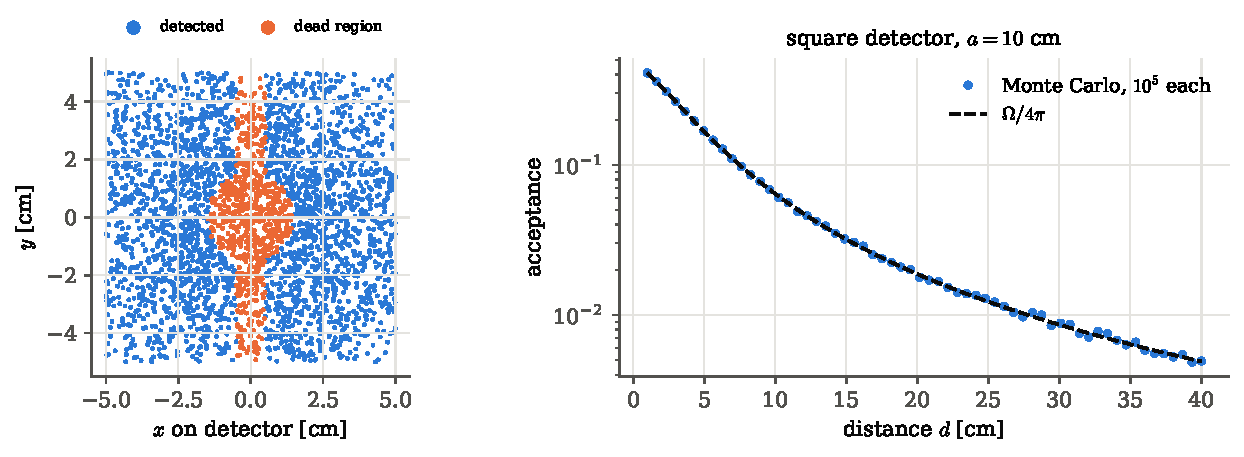
\includegraphics[width=\linewidth]{figures/ch06/acceptance.pdf}
\caption{Detector acceptance by Monte Carlo. Left: where the particles that reach the
square cross it, for $d=5\,$cm; those in the dead strip and the central hole (orange) are
lost. Right: acceptance of the plain square against distance, $10^5$ particles per point,
on the exact $\Omega/4\pi$ of \eqref{6b:eq:solidangle}.}
\label{6b:fig:acceptance}
\end{figure}

\begin{inpractice}[Why physics runs on sampling]
The two uses of the acceptance calculation are the two uses of Monte Carlo in research.
Against \eqref{6b:eq:solidangle} it \emph{verifies}: the code, the random numbers and the
error bars are checked against a known answer. With the dead strip it \emph{is the
answer}: no formula exists and the simulation is the instrument. A collider analysis
chains the two stages Cowan describes \srcref{Cowan}{\S3.4}. An \newterm{event generator}
such as \textsc{Pythia} \cite{Pythia83} samples the four-momenta of the final-state particles
from the differential cross section: hard scattering, parton showers and hadronisation,
each by inverse-CDF, rejection and veto steps of exactly the kinds in this chapter. A
\newterm{detector simulation} such as \textsc{Geant4} \cite{Geant4} then samples each
particle's interactions with the material: ionisation, multiple scattering, showers. The
output is treated like real data: it gives the acceptance and efficiency, the response
matrix for unfolding, and the distribution of a test statistic under the background-only
hypothesis (\cref{ch:04}). In cosmology the same role is played by simulated skies pushed
through the mask, beam and noise of the instrument (\cref{ch:08}). In the pipeline from physical model to inference, sampling is how we
\emph{derive the sampling distribution of a summary} whenever the
algebra gives out.
\end{inpractice}
\section{Importance sampling, and why $g$ needs thicker tails than $f$}
\label{6b:sec:importance}

A search for a rare background fluctuation needs the probability that a standard normal
test statistic exceeds $3$, $\Prob(Z>3)=\SixBIsTailP$. Estimated by plain Monte Carlo
with $N=\SixBIsTailN$ draws, it is the fraction of draws above $3$ (\cref{6b:sec:sqrtN}).
Most runs of $100$ draws contain no such draw at all: in $\SixBIsTailR$ repeated runs, a
fraction $\SixBIsPlainZero$ returned exactly zero. Why? The integrand is the indicator
$h(x)=\mathbf 1[x>3]$, equal to $1$ above $3$ and $0$ below. Nearly every draw lands
below $3$, where $h$ is zero, and tells us nothing. So the trouble is not the factor
$1/\sqrt N$ but the constant $\sigma$ in front of it: we sampled from a density that
rarely visits the region that matters.

A second problem has the same shape. In Bayesian inference the density we need to
average over, the posterior, is usually one we cannot sample at all, while a simpler
density that resembles it is easy to sample \mainref{\S24.3}. Both problems have the
same fix: draw from a density of our choosing, and correct each draw with a weight.

\paragraph{The question.} If we draw from a density $g$ instead of $f$, how do we still
estimate $\int hf$, and which $g$ make the estimate better or worse?

\subsection{Reweighting}
\label{6b:sec:is-derive}

Let $g$ be any density that is positive wherever $h(x)f(x)\ne0$. Multiply and divide by it
\mainref{(24.4)}:
\begin{align}
  I=\int h(x)f(x)\,\dd x
  \eqby{1}\int\frac{h(x)f(x)}{g(x)}\,g(x)\,\dd x
  \eqby{2}\E_g\Bigl[h(X)\,w(X)\Bigr],\qquad w(x)\equiv\frac{f(x)}{g(x)} .
  \label{6b:eq:is}
\end{align}
\begin{explain}
  \item Multiplying and dividing by $g(x)$ changes nothing where $g>0$; where $g=0$ the
        integrand $hf$ vanishes by assumption, so no part of the integral is lost.
  \item An integral against the density $g$ is an expectation under $g$.
\end{explain}
So draw $X_1,\dots,X_N\sim g$ and average the weighted values \mainref{(24.5)}:
\begin{equation}
  \hat I_g=\frac1N\sum_{i=1}^Nh(X_i)\,w(X_i) .
  \label{6b:eq:is-est}
\end{equation}
The \newterm{importance weight} $w=f/g$ \unpack{how much more often $f$ would have produced
this value than $g$ did} corrects for sampling from the wrong density: values that $g$
over-produces get weights below one, values it under-produces get weights above one. By
\eqref{6b:eq:mc-var} applied to the terms $hw$ under $g$, $\hat I_g$ is unbiased and its
variance is $\Var_g[hw]/N$, with \mainref{(24.6)}
\begin{align}
  \Var_g[hw]
  \eqby{1}\E_g\bigl[h^2w^2\bigr]-I^2
  \eqby{2}\int\frac{h^2(x)f^2(x)}{g^2(x)}\,g(x)\,\dd x-I^2
  \eqby{3}\int\frac{h^2(x)f^2(x)}{g(x)}\,\dd x-I^2 .
  \label{6b:eq:is-var}
\end{align}
\begin{explain}
  \item Variance is the mean square minus the square of the mean, and the mean of $hw$
        under $g$ is $I$ by \eqref{6b:eq:is}.
  \item Write the expectation under $g$ as an integral, with $w=f/g$.
  \item One factor of $g$ cancels.
\end{explain}
Everything about the quality of importance sampling is in the last integral, and the
key feature is that $g$ sits in its \emph{denominator}. Where $g$ is much smaller than
$f$ (and $h\ne0$), the integrand $h^2f^2/g$ is large. If $g$ falls off faster than $f$ in
the tails, the integrand grows there instead of dying away, and the integral diverges.

\begin{workdef}[importance sampling]
To estimate $I=\int hf$, draw $X_i\sim g$ and average $h(X_i)\,f(X_i)/g(X_i)$
\unpack{each draw weighted by how much likelier it is under $f$ than under $g$}.
\emph{Unbiased} whenever $g>0$ where $hf\ne0$. \emph{Standard error}
$\sqrt{(\int h^2f^2/g-I^2)/N}$, estimated by the sample standard deviation of the
$h_iw_i$ over $\sqrt N$ when it is finite.
\end{workdef}

\subsection{The tail rule, shown}
\label{6b:sec:tail-rule}

We can see the divergence in the simplest possible case. Let the target be the standard
normal, $f=\Normal(0,1)$, and estimate its normalisation: take $h=1$, so $I=\int f=1$.
Put another way, if we knew only the unnormalised curve $e^{-x^2/2}$, we would be
estimating its area $Z=\sqrt{2\pi}$, and the ratio $\hat Z/Z$ is the same number as
$\hat I$. This is the evidence problem of \cref{ch:05} in miniature. Sample from
$g=\Normal(0,s^2)$, a Gaussian of adjustable width $s$. With $h=1$ the second moment of
the terms in \eqref{6b:eq:is-var} is the mean square weight,
\begin{align}
  \E_g[w^2]=\int\frac{f^2}{g}\,\dd x
  &\eqby{1}\int\frac{e^{-x^2}/2\pi}{e^{-x^2/2s^2}/\sqrt{2\pi}\,s}\,\dd x
   \eqby{2}\frac{s}{\sqrt{2\pi}}\int\exp\Bigl[-x^2\Bigl(1-\frac1{2s^2}\Bigr)\Bigr]\dd x
   \nonumber\\
  &\eqby{3}\frac{s}{\sqrt{2\pi}}\sqrt{\frac{\pi}{1-1/2s^2}}
   \eqby{4}\frac{s^2}{\sqrt{2s^2-1}}\qquad\text{if } s^2>\tfrac12,
  \qquad\text{and } \infty \text{ if } s^2\le\tfrac12 .
  \label{6b:eq:gauss-is}
\end{align}
\begin{explain}
  \item $f^2=e^{-x^2}/2\pi$ and $g=e^{-x^2/2s^2}/(\sqrt{2\pi}\,s)$.
  \item Collect the constants and the exponents: $-x^2+x^2/2s^2$.
  \item $\int e^{-cx^2}\dd x=\sqrt{\pi/c}$ for $c>0$. If $c=1-1/2s^2\le0$ the integrand does
        not decay and the integral is infinite.
  \item $s\sqrt{1/(2-1/s^2)}=s\cdot s/\sqrt{2s^2-1}$.
\end{explain}
Since $I=1$, the variance of one weight is $\E_g[w^2]-1=s^2/\sqrt{2s^2-1}-1$, and this
is also its variance relative to the answer. It is zero at $s=1$, when $g=f$ and every
weight is exactly $1$. For $s>1$ ($g$ wider than $f$) it grows only slowly:
at $s=1.5$ it is $\SixBIsThickRelVar$. For $s<1$ ($g$ narrower) it grows fast and becomes
infinite at $s=1/\sqrt2$, although $g$ is still a perfectly good Gaussian that covers the
whole real line. \Cref{6b:fig:is-tails} shows the measured scatter of $\hat Z/Z$ over
$400$ runs of $N=1000$ draws against $s$: on the theory curve for $s>1/\sqrt2$, erratic and
large below.

\begin{figure}[htbp]
\centering
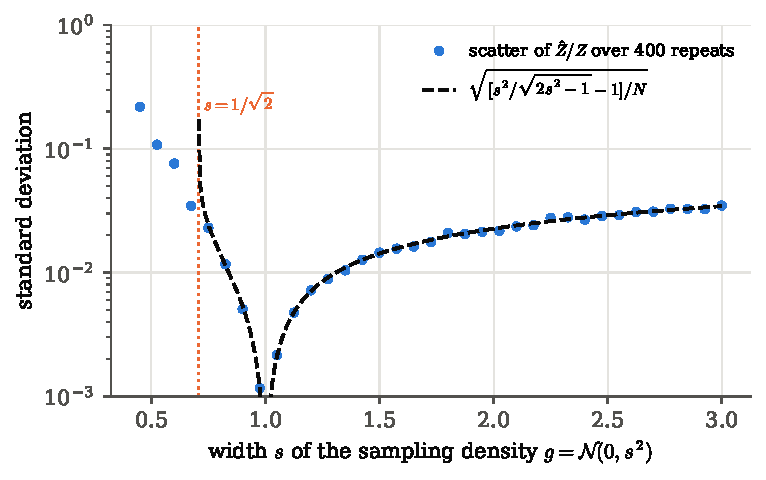
\includegraphics[width=0.62\linewidth]{figures/ch06/importance_tails.pdf}
\caption{How the width of the sampling density controls importance sampling. Each point is
the standard deviation of the estimate of the normalisation of a standard normal, from $400$
runs of $1000$ draws from $g=\Normal(0,s^2)$. It vanishes at $s=1$ ($g=f$), rises gently for
wider $g$, and diverges at $s=1/\sqrt2$; below that the variance is infinite and the scatter
over a finite number of runs is erratic.}
\label{6b:fig:is-tails}
\end{figure}

What does an infinite variance look like in a single run? The weights are
$w=f/g=s\,e^{x^2(1/2s^2-1/2)}$. For $s=0.5$ that is $\tfrac12e^{3x^2/2}$: modest near
the centre, and astronomically large for the rare draw far out in the tail of $g$. The mean
of $w$ is still finite, so the estimate still converges, by the law of large numbers. But
the central limit theorem needs a finite variance, so it no longer applies, and the
error does not shrink as $1/\sqrt N$. In practice, most of the time the running estimate
sits a little \emph{low}, because the large weights that should balance it have not been
drawn yet. Then one draw lands in the tail and the estimate jumps
(\cref{6b:fig:is-running}, left). With
$\SixBIsNrun$ draws, three independent runs at $s=0.5$ end with a spread of
$\SixBIsThinSpread$ in $\hat Z/Z$, against $\SixBIsThickSpread$ at $s=1.5$. The
\newterm{effective sample size} $(\sum w_i)^2/\sum w_i^2$ \unpack{the number of equally
weighted draws that would carry the same information} is a fraction $\SixBIsThinEss$ of $N$ at
$s=0.5$ and $\SixBIsThickEss$ at $s=1.5$.

\begin{keyidea}[Thicker tails than the target]
A basic rule in importance sampling is to sample from a density $g$ with thicker tails
than $f$ \mainref{p.~409}. The variance of the estimate contains $\int h^2f^2/g$, with $g$ in
the denominator. If $g$ falls off faster than $f$, the weights $f/g$ grow without bound in the
tails and the variance is infinite. A good $g$ is similar in shape to $f$ (or to $\lvert
h\rvert f$) and a little wider.
\end{keyidea}

\begin{figure}[htbp]
\centering
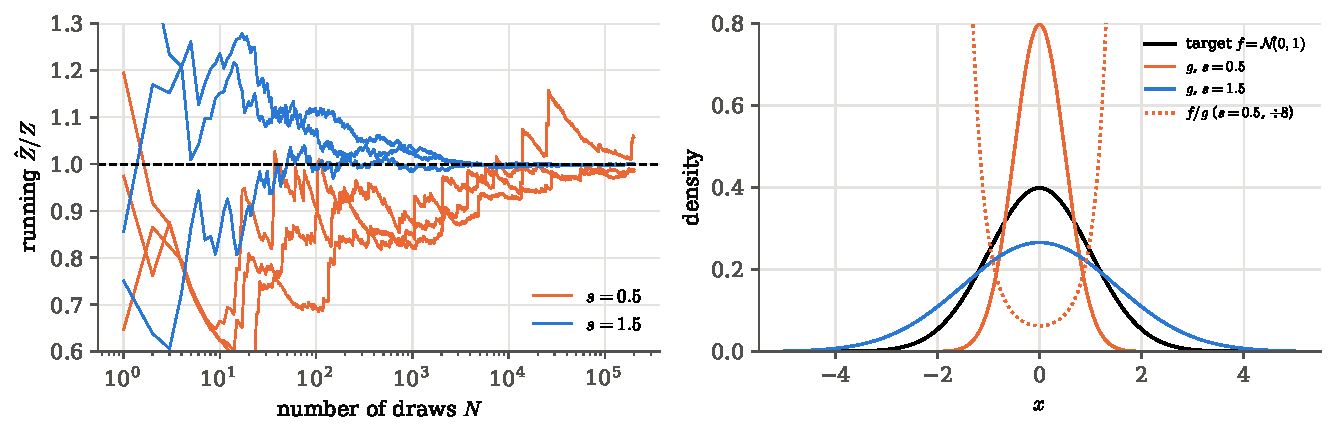
\includegraphics[width=\linewidth]{figures/ch06/importance_running.pdf}
\caption{Left: running estimates of the normalisation of a standard normal, three runs each,
with a narrow sampling density ($s=0.5$, orange) and a wide one ($s=1.5$, blue). The narrow
one drifts and jumps whenever a rare tail draw arrives with a huge weight. Right: the target
and the two sampling densities; the dotted curve is the weight $f/g$ for $s=0.5$ (scaled down
by $8$), which grows without bound in the tails.}
\label{6b:fig:is-running}
\end{figure}

\begin{pitfall}[The error bar lies before the estimate does]
With infinite variance the sample standard deviation of the weights is finite in every run,
so $s/\sqrt N$ always prints a number. It is too small most of the time, because the draws
that would reveal the true spread are the rare ones that have not happened yet. Check the
effective sample size and the largest single weight's share of the total, and plot the running
estimate.
\end{pitfall}

\subsection{The best $g$, and a tail probability}
\label{6b:sec:is-optimal}

Which $g$ minimises the variance? In \eqref{6b:eq:is-var} the term $I^2$ is fixed, so only
the second moment $\E_g[h^2w^2]$ depends on $g$. We first find a floor below which it
cannot go, whatever $g$ we pick. The tool is the inequality $\E[Y^2]\ge(\E\lvert Y\rvert)^2$,
a case of Jensen's inequality, which holds because the variance of $\lvert Y\rvert$ cannot be
negative. With $Y=hw$ it gives
\begin{align}
  \E_g\bigl[h^2w^2\bigr]
  \relby{1}{\ge}\Bigl(\E_g\bigl[\lvert h\rvert w\bigr]\Bigr)^2
  \eqby{2}\Bigl(\int\lvert h(x)\rvert\,\frac{f(x)}{g(x)}\,g(x)\,\dd x\Bigr)^2
  \eqby{3}\Bigl(\int\lvert h\rvert f\,\dd x\Bigr)^2 .
  \label{6b:eq:jensen}
\end{align}
\begin{explain}
  \item $\E[Y^2]-(\E\lvert Y\rvert)^2=\Var\lvert Y\rvert\ge0$, with $Y=hw$.
  \item Write the expectation as an integral against $g$.
  \item $g$ cancels.
\end{explain}
Can any $g$ reach this floor? Equality needs $\lvert h\rvert w$ to have zero variance, that
is, to take the same value at every draw. The choice
$g^*(x)=\lvert h(x)\rvert f(x)/\int\lvert h\rvert f$ does exactly that: then
$\lvert h\rvert w=\lvert h\rvert f/g^*=\int\lvert h\rvert f$ for every draw \mainref{Thm~24.5}. For
$h\ge0$ the estimator itself then has zero variance: every single draw returns the exact
answer. This is only of theoretical interest. To normalise $g^*$ we need
$\int\lvert h\rvert f$, which is the integral we wanted in the first place
\mainref{p.~410}. What it teaches in practice is a guideline: make $g$ resemble
$\lvert h\rvert f$, the place where the integrand actually lives, and give it thicker tails.

\paragraph{Example: $\Prob(Z>3)$.}
For $h=\mathbf 1[x>3]$ and $f=\Normal(0,1)$, the ideal $g^*$ is the normal density truncated to
$x>3$. A simple imitation is $g=\Normal(4,1)$, centred beyond the threshold
\mainref{Ex.~24.6}. The weight is $w=f/g=\exp[-x^2/2+(x-4)^2/2]=e^{8-4x}$, and the second moment
of the estimator's terms can be done exactly:
\begin{align}
  \E_g[h^2w^2]
  \eqby{1}\int_3^\infty\frac{f^2}{g}\,\dd x
  \eqby{2}\int_3^\infty\frac{1}{\sqrt{2\pi}}\,e^{-x^2+(x-4)^2/2}\,\dd x
  \eqby{3}e^{16}\int_3^\infty\frac{e^{-(x+4)^2/2}}{\sqrt{2\pi}}\,\dd x
  \eqby{4}e^{16}\bigl[1-\Phi(7)\bigr] .
  \label{6b:eq:tail-is}
\end{align}
\begin{explain}
  \item \eqref{6b:eq:is-var} with $h^2=h=\mathbf 1[x>3]$.
  \item $f^2/g=\bigl(e^{-x^2}/2\pi\bigr)\big/\bigl(e^{-(x-4)^2/2}/\sqrt{2\pi}\bigr)$.
  \item Complete the square: $-x^2+\tfrac12(x-4)^2=-\tfrac12x^2-4x+8=-\tfrac12(x+4)^2+16$.
  \item Substitute $t=x+4$: the integral is the normal tail beyond $7$.
\end{explain}
This is $\SixBIsSecond$, so the standard deviation of $\hat I_g$ with $N=100$ is
$\sqrt{(\SixBIsSecond-p^2)/100}=\SixBIsIsSdTh$, against the plain binomial
$\sqrt{p(1-p)/100}=\SixBIsPlainSdTh$. Over $\SixBIsTailR$ repeated runs the script measures
$\SixBIsPlainSd$ for plain Monte Carlo and $\SixBIsIsSd$ for importance sampling, a gain of
$\SixBIsGain$ in standard deviation, or about $140$ in the number of draws needed for a given
precision.\footnote{Wasserman reports the reduction as ``a factor of 20''
\mainref{p.~410}, from simulated values $0.0039$ and $0.0002$ that he labels as variances but
that are standard deviations. (A variance of $0.0039$ is impossible here: the plain estimator's variance is
$p(1-p)/100\approx1.3\times10^{-5}$.) The exact standard deviations from \eqref{6b:eq:tail-is}
are $0.0037$ and $0.00031$, a factor of $11.9$, which our simulation reproduces; his second
value, $0.0002$, is low, and the ratio of his rounded numbers, $19.5$, is quoted as $20$.} The means of the two estimators are $\SixBIsPlainMean$ and $\SixBIsIsMean$, both
unbiased for $p=\SixBIsTailP$.

The same device is how particle physicists reweight simulated events. Events generated
under one set of parameters (a parton distribution set, a value of a coupling, a
Wilson coefficient) are reused for another by the weight $w=f_{\text{new}}/f_{\text{old}}$ of
each event's kinematics, and the effective sample size tells us when the old sample is too
far from the new model to be trusted. The tail rule applies exactly: reweighting towards a
harder spectrum than the one generated puts huge weights on the few high-energy events.

\subsection{Self-normalised importance sampling for posteriors}
\label{6b:sec:self-norm}

For a posterior we know $f(\theta)\propto\Like(\theta)\pi(\theta)$, the likelihood times
the prior, only up to the evidence, which is the unknown normalising constant. So
importance sampling as written cannot be used directly: the weight $f/g$ needs $f$
itself. The way round it is to work with the unnormalised posterior $\tilde f=\Like\pi$
and the weight $w=\tilde f/g$. The posterior mean is a ratio of two integrals, and each
can be estimated from the same draws $\theta_j\sim g$ \mainref{Ex.~24.7}:
\begin{align}
  \E[\theta\given\data]
  \eqby{1}\frac{\int\theta\,\tilde f(\theta)\,\dd\theta}{\int\tilde f(\theta)\,\dd\theta}
  \eqby{2}\frac{\E_g[\theta\,w(\theta)]}{\E_g[w(\theta)]}
  \;\approx\;\frac{\sum_j\theta_j\,w_j}{\sum_jw_j} .
  \label{6b:eq:selfnorm}
\end{align}
\begin{explain}
  \item The evidence $\int\tilde f$ normalises the posterior, so it divides the unnormalised
        integral.
  \item Importance sampling \eqref{6b:eq:is} applied to numerator and denominator
        separately.
\end{explain}
The unknown constant cancels between numerator and denominator. The price is a small
bias: a ratio of two unbiased averages is not itself unbiased for finite $N$. The bias
vanishes as $N$ grows (the estimator is \newterm{consistent}), and the tail rule applies to
it just as before.

\paragraph{Example: a measurement with an outlier.}
Model three measurements as $x_i=\theta+\epsilon_i$ with Student-$t$ noise of $\nu=3$ degrees of
freedom, a heavy-tailed noise model that tolerates occasional wild values
\mainref{Ex.~24.7}, and a flat prior on $\theta$. Take the data $x=(\SixBIsPostXa,\SixBIsPostXb,
\SixBIsPostXc)$, where the first point is an outlier. The posterior mean, by numerical
quadrature, is $\SixBIsPostTrue$.

\emph{The tails decide the sampler.} The $t_3$ density is proportional to
$(1+t^2/3)^{-2}$, so each likelihood factor falls off as $\lvert\theta\rvert^{-4}$, and the
posterior, a product of three such factors, has polynomial tails
$\propto\lvert\theta\rvert^{-12}$. Try $g=\Normal(0,1)$, whose tails are Gaussian: the weight
$\tilde f/g$ grows like $e^{\theta^2/2}\lvert\theta\rvert^{-12}$, and the variance
\eqref{6b:eq:is-var} is infinite. Try $g=\mathrm{Cauchy}(0,1)$, with tails
$\propto\theta^{-2}$, heavier than the posterior's: the weight is bounded.

\emph{The numbers.} Over $2000$ runs of $1000$ draws each, the Normal sampler gives estimates
with median $\SixBIsPostNormMed$, standard deviation $\SixBIsPostNormSd$ and a $1$--$99\%$ range
$[\SixBIsPostNormLo,\SixBIsPostNormHi]$; the Cauchy sampler gives median $\SixBIsPostCauchyMed$,
standard deviation $\SixBIsPostCauchySd$ and range $[\SixBIsPostCauchyLo,\SixBIsPostCauchyHi]$.
The typical Normal-sampler answer is pulled towards the bulk of the data. The reason is
that the region around the outlier, which pulls the posterior mean down, is almost never
sampled. Wasserman's
two-point version shows the same: $-0.74$ from a Normal sampler and $-0.53$ from a Cauchy sampler,
against the true $-0.54$ \mainref{p.~411}.

\pyfile[firstline=120,lastline=125,firstnumber=120]{code/ch06/27_importance.py}{Self-normalised
importance sampling of a posterior mean}

Line 124 is the weight, the unnormalised posterior over the sampling density, and line 125 is
\eqref{6b:eq:selfnorm}. Nothing in the loop knows the evidence.

Importance sampling returns in the rest of the book. Nested sampling and the evidence
estimators of \cref{ch:05} are importance sampling with cleverly chosen $g$. An MCMC chain
(\cref{ch:09}) can be reweighted to a slightly different prior or likelihood with the weights
$p_{\text{new}}/p_{\text{old}}$, subject to the same tail rule. And Casella and Berger's
condition $M<\infty$ for rejection sampling (\cref{6b:sec:reject-limits}) is the same requirement
in its strongest form: rejection needs $f/g$ bounded, importance sampling needs only
$\int f^2/g<\infty$.
\section{A histogram of samples approximates the density}
\label{6b:sec:histogram}

To see the distribution that a pile of samples came from, we histogram them. Every method
so far ends with such a pile: decay times, directions, posterior draws of the difference
$\delta=p_2-p_1$ of two efficiencies. From \cref{ch:09} on, a Markov chain will hand us a
pile of parameter values and nothing else, with no formula for the posterior at all.
Wasserman states the idea for posterior draws: if
$\theta_1,\dots,\theta_B$ are drawn from $p(\theta\given\data)$, then a histogram of
$\theta_1,\dots,\theta_B$ approximates the posterior density \mainref{\S11.4, p.~180}.
Kruschke builds his whole approach to Bayesian computation on it. A distribution is
represented by a large sample of representative values, as an opinion poll represents a
population, and the larger the sample, the better the representation
\srcref{Kruschke}{\S7.1}.

The idea is not special to posteriors. It also gives the probability distribution of the
position of a particle: we plot the histogram of $x$ for a large set of random values of the
time $t$. Take a classical oscillator $x(t)=A\cos\omega t$, observed at a random moment.
It is found at position $x$ with some probability density, and we can obtain that density
without any algebra: sample many random times, compute $x$ at each, and histogram. Here the
sampling prescription is ``the time is uniform''. As \cref{1b:ex:arcsine} showed, the
equation of motion alone fixes no distribution; choosing the position uniformly instead
would give a different one.

\paragraph{The question.} How close is a histogram of $N$ samples to the density that
produced them, and what error bar belongs on each bin?

\subsection{What a bin count is}
\label{6b:sec:bin-count}

Divide the range into bins of width $\Delta$, and let bin $k$ be the interval
$[b_k,b_{k+1})$. Each sample falls into bin $k$ with probability
\[
  p_k=\int_{b_k}^{b_{k+1}}f(x)\,\dd x=F(b_{k+1})-F(b_k),
\]
independently of the other samples. So the count $n_k$ in bin $k$ is the number of successes
in $N$ independent trials with success probability $p_k$: it is
$\mathrm{Binomial}(N,p_k)$ (\cref{ch:02}). The natural estimate of the density is the
fraction of samples in the bin per unit length, $\hat f_k=n_k/(N\Delta)$.

\begin{workdef}[histogram density estimate]
$\hat f_k=n_k/(N\Delta)$ \unpack{the fraction of the $N$ samples that fell in bin $k$, divided
by the bin width}. It estimates the \emph{bin-averaged} density $p_k/\Delta$, with standard
error
\[
  \delta\hat f_k=\frac{\sqrt{N p_k(1-p_k)}}{N\Delta}\approx\frac{\sqrt{n_k(1-n_k/N)}}{N\Delta}
  \approx\frac{\sqrt{n_k}}{N\Delta}\quad(p_k\ll1).
\]
\end{workdef}

The mean and variance follow from those of the binomial:
\begin{align}
  \E[\hat f_k]\eqby{1}\frac{\E[n_k]}{N\Delta}\eqby{2}\frac{Np_k}{N\Delta}=\frac{p_k}{\Delta},
  \qquad
  \Var[\hat f_k]\eqby{3}\frac{\Var[n_k]}{N^2\Delta^2}\eqby{4}\frac{p_k(1-p_k)}{N\Delta^2},
  \qquad
  \frac{\delta\hat f_k}{\E[\hat f_k]}\eqby{5}\sqrt{\frac{1-p_k}{Np_k}} .
  \label{6b:eq:bin-error}
\end{align}
\begin{explain}
  \item $N\Delta$ is a constant.
  \item A binomial count has mean $Np_k$.
  \item A constant factor comes out of a variance squared.
  \item A binomial count has variance $Np_k(1-p_k)$.
  \item The standard deviation divided by the mean.
\end{explain}
So the relative error of a bin is about $1/\sqrt{Np_k}$, one over the square root of the
expected count in that bin. A bin expected to hold $100$ samples is good to $10\%$, whatever
$N$ is. When there are many bins, each $p_k$ is small, $1-p_k\approx1$, and the binomial is
close to a Poisson distribution with mean $Np_k$. This gives the familiar $\sqrt n$ error bar.

Are the bins independent of each other? With $N$ fixed, not quite: the counts must add up to
$N$, so a sample in one bin is a sample missing from the others. They are multinomial and
slightly anticorrelated, $\Cov(n_j,n_k)=-Np_jp_k$, which is negligible when all the $p_k$ are
small. If $N$ is itself a Poisson count, as in a counting experiment with a fixed exposure,
the bin counts are exactly independent Poisson variables.

What a bin estimates is the density \emph{averaged over the bin}, not its value at the centre.
Expand $f$ about the bin centre $c$ to see the difference:
\begin{align}
  \frac{p_k}{\Delta}
  \eqby{1}\frac1\Delta\int_{-\Delta/2}^{\Delta/2}f(c+s)\,\dd s
  \eqby{2}\frac1\Delta\int_{-\Delta/2}^{\Delta/2}\Bigl[f(c)+f'(c)\,s+\tfrac12f''(c)\,s^2+\dots\Bigr]\dd s
  \eqby{3}f(c)+\frac{\Delta^2}{24}f''(c)+\dots
  \label{6b:eq:bin-bias}
\end{align}
\begin{explain}
  \item Substitute $x=c+s$ in the integral over the bin.
  \item Taylor expansion of $f$ about the centre.
  \item The linear term integrates to zero over a symmetric interval, and
        $\int_{-\Delta/2}^{\Delta/2}s^2\,\dd s=\Delta^3/12$.
\end{explain}
So a histogram is biased by $\Delta^2f''/24$ as an estimate of $f$ at the bin centres, and the
bias is largest where the density curves sharply.

How wide should the bins be? Narrow bins reduce the bias but, by \eqref{6b:eq:bin-error},
raise the relative error, since each bin holds fewer samples. The squared bias falls like
$\Delta^4$ and the variance rises like $1/(N\Delta)$. Their sum is smallest where the two
are balanced, $\Delta^4\propto1/(N\Delta)$, that is $\Delta\propto N^{-1/5}$. Both terms are
then of order $N^{-4/5}$, so the error falls like $N^{-2/5}$: the histogram converges to
the density more slowly than $1/\sqrt N$. For comparing a histogram with a model, the
bias can be avoided altogether: compare $n_k$ with the model's expected count $Np_k$
computed from the CDF, which is exact for any bin width.

\subsection{The oscillator seen at random times}
\label{6b:sec:oscillator}

We now put the histogram to work on the oscillator of the opening of this section,
$x(t)=A\cos\omega t$ with amplitude $A$ and angular frequency $\omega$. We pick the
observation time $t$ uniformly over one period $T=2\pi/\omega$. To have something to
compare the histogram with, we first need the exact density of $x$. It follows from the
change of variables of \cref{ch:01}. Each value of $x$ in $(-A,A)$ is reached at two times
per period, once moving left and once moving right, and at each of them the speed is
$\lvert\dd x/\dd t\rvert=A\omega\lvert\sin\omega t\rvert=\omega\sqrt{A^2-x^2}$:
\begin{align}
  p(x)
  \eqby{1}\sum_{\text{2 times}}p_t(t)\,\Bigl\lvert\frac{\dd t}{\dd x}\Bigr\rvert
  \eqby{2}2\cdot\frac1T\cdot\frac{1}{\omega\sqrt{A^2-x^2}}
  \eqby{3}\frac{1}{\pi\sqrt{A^2-x^2}},
  \qquad
  F(x)\eqby{4}\frac12+\frac1\pi\arcsin\frac xA .
  \label{6b:eq:arcsine}
\end{align}
\begin{explain}
  \item The probability of finding $x$ in $\dd x$ is the probability that $t$ falls in the
        time intervals that map onto $\dd x$, summed over both branches.
  \item $t$ is uniform over the period, $p_t=1/T$, and the speed is the same on both
        branches.
  \item $\omega T=2\pi$.
  \item Integrate: $\int\dd x/\sqrt{A^2-x^2}=\arcsin(x/A)$, with $F(-A)=0$.
\end{explain}
This is the arcsine density of \cref{1b:ex:arcsine}. It diverges at the turning points
$x=\pm A$, where the oscillator is slow and spends most of its time. It is lowest at the
centre, where the oscillator moves fastest. The divergence is integrable, so the total
probability is still one. Classical statistical mechanics makes the same statement: picking a
random time is the same as picking a random point on the phase-space orbit, so the fraction of
time the system spends in a region is the probability of finding it there. A Markov chain
(\cref{ch:09}) uses exactly this: the fraction of time the chain spends in a region is its
estimate of the region's probability.

\pyfile[firstline=30,lastline=41,firstnumber=30]{code/ch06/28_histogram_density.py}{The
oscillator position at random times, histogrammed with binomial error bars}

Line 31 draws the random times and line 32 evaluates the trajectory at each; nothing else is
needed to generate the distribution. Lines 33--38 build the histogram and convert counts into
a density. Line 37 computes the exact bin probabilities $p_k$ from the CDF
\eqref{6b:eq:arcsine}, line 39 the error bars of \eqref{6b:eq:bin-error}, and lines 40--41 the
pull of each bin and the $\chi^2$ of the whole histogram.

\paragraph{Example: how good is it?}
With $N=\SixBHoN$ random times and $K=\SixBHoK$ bins on $[-A,A]$
(\cref{6b:fig:oscillator}), the Pearson statistic $\sum_k(n_k-Np_k)^2/Np_k$ is $\SixBHoChi$
for $\SixBHoDof$ degrees of freedom ($K$ bins minus one, because the counts must add up to
$N$), a $p$-value of $\SixBHoPval$ (\cref{ch:04}). The pulls $(n_k-Np_k)/\sqrt{Np_k(1-p_k)}$ have
standard deviation $\SixBHoPullSd$, close to one, which says that the binomial error bars are
the right size. The relative error in a central bin is $\SixBHoRelErrMid$ and in the end bin
$\SixBHoRelErrEdge$, because the end bins hold many more samples.

\paragraph{Example: the bin average is not the value at the centre.}
In the central bin the bin-averaged density $p_k/\Delta=\SixBHoMidAvg$ equals the density at
the centre, $\SixBHoMidCen$, to four digits, because the density is flat there. In the last bin,
$[0.95A,A)$, the average is $\SixBHoEdgeAvg/A$ while the density at the bin centre is only
$\SixBHoEdgeCen/A$: the divergence at $x=A$ lies inside the bin, and the Taylor expansion
\eqref{6b:eq:bin-bias} fails completely there. A histogram drawn over the curve
$1/\pi\sqrt{A^2-x^2}$ therefore seems to overshoot at the ends, and a $\chi^2$ against the density at the
bin centres would reject a perfect sample. The green staircase in \cref{6b:fig:oscillator},
the exact bin averages, is what the histogram estimates.

\begin{figure}[htbp]
\centering
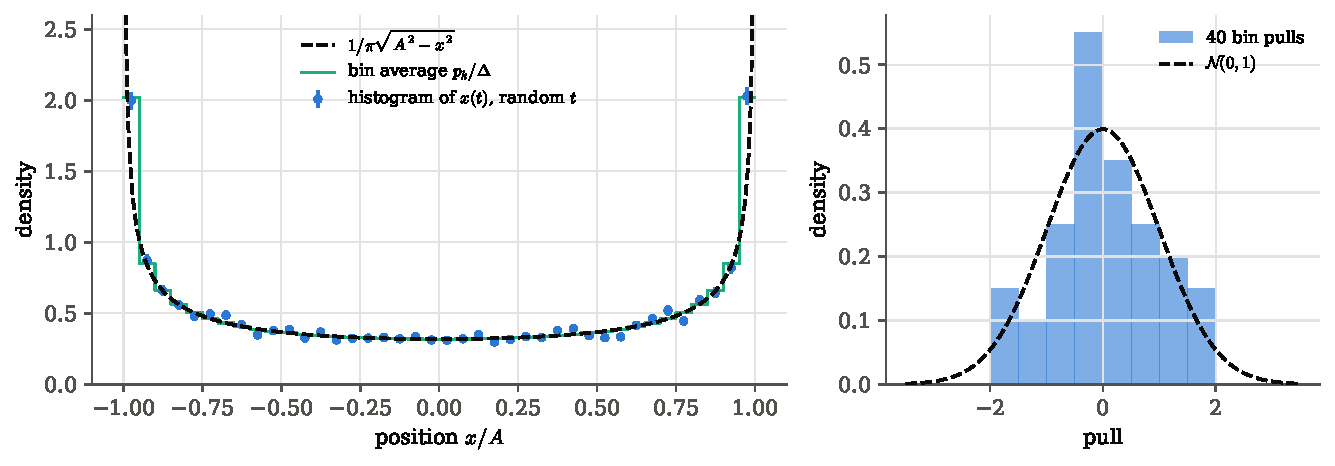
\includegraphics[width=\linewidth]{figures/ch06/oscillator_histogram.pdf}
\caption{The position of a classical oscillator at $10^4$ random times. Left: the histogram as
a density with binomial error bars, the arcsine density (black dashed) and its exact bin
averages (green staircase); the histogram follows the staircase, which lies above the curve in
the end bins because the density diverges inside them. Right: the pulls of the $40$ bins are
distributed as a standard normal.}
\label{6b:fig:oscillator}
\end{figure}

\paragraph{Example: summaries from a representative sample.}
Kruschke's illustration represents a $\mathrm{Beta}(15,7)$ density, which could be the posterior
for the probability of heads after $14$ heads in $20$ tosses with a flat prior, by random samples
of increasing size \srcref{Kruschke}{Fig.~7.1}. The exact mode is $\SixBKrModeExact$ and the exact
$95\%$ highest-density interval (the shortest interval holding $95\%$ of the probability,
\cref{ch:05}) is $[\SixBKrLoExact,\SixBKrHiExact]$. From the samples we estimate the mode as the
centre of the tallest histogram bin and the HDI as the shortest interval containing $95\%$ of the
sorted draws. With $N=\SixBKrNA$ the script finds a mode of $\SixBKrModeA$ and an HDI of
$[\SixBKrLoA,\SixBKrHiA]$; with $N=\SixBKrNB$, $\SixBKrModeB$ and $[\SixBKrLoB,\SixBKrHiB]$; with
$N=\SixBKrNC$, $\SixBKrModeC$ and $[\SixBKrLoC,\SixBKrHiC]$ (\cref{6b:fig:beta-samples}). The
interval limits settle to within $0.01$ of the exact ones at $N=5000$, as the $1/\sqrt N$ law
predicts. The mode is the slowest summary to settle, because it depends on the height of a
single bin, which is the noisiest thing a histogram offers. Kruschke's numbers ($0.723$ and
$[0.477,0.875]$ at $N=500$) scatter about the truth in the same way.

\begin{figure}[htbp]
\centering
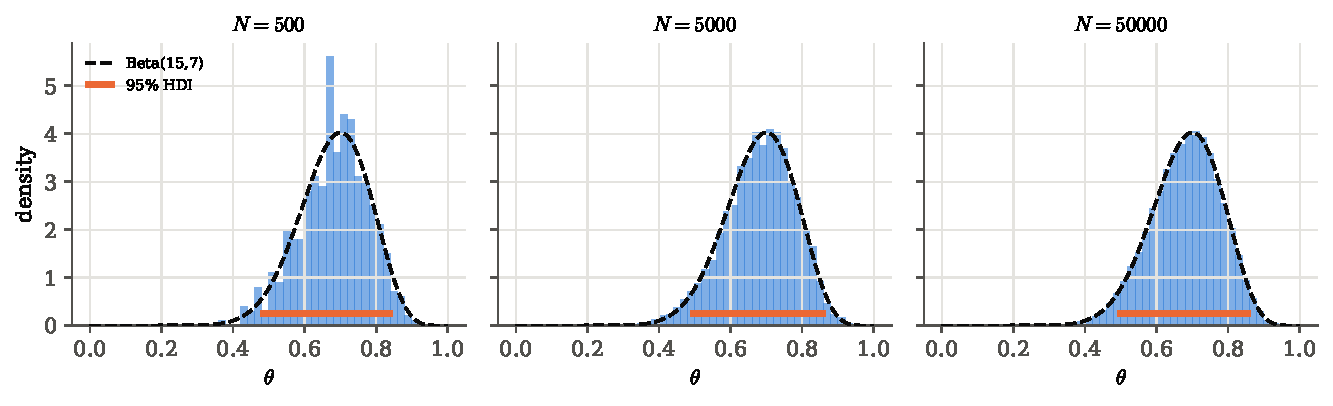
\includegraphics[width=\linewidth]{figures/ch06/beta_samples.pdf}
\caption{A $\mathrm{Beta}(15,7)$ density represented by $500$, $5000$ and $50\,000$ random
samples, with the $95\%$ highest-density interval found from each sample (orange bar). The
histogram becomes smoother and the interval converges on the exact one as $N$ grows.}
\label{6b:fig:beta-samples}
\end{figure}

\begin{pitfall}[Empty bins and the density at the centre]
Two mistakes are common when a simulated histogram is compared with a model. The first is to
compare $n_k/(N\Delta)$ with $f$ at the bin centre instead of with $p_k/\Delta$; it fails wherever
$f$ curves sharply or diverges. The second is to put bins with zero or very few expected counts
into a Pearson $\chi^2$, where the Gaussian approximation behind $\chi^2$ fails; use the
Poisson likelihood of \cref{ch:03} instead, or merge the sparse bins.
\end{pitfall}
\providecommand{\SixBUfM}{}\renewcommand{\SixBUfM}{20}
\providecommand{\SixBUfMuTot}{}\renewcommand{\SixBUfMuTot}{20\,000}
\providecommand{\SixBUfNmc}{}\renewcommand{\SixBUfNmc}{2\times10^{6}}
\providecommand{\SixBUfSigmaBins}{}\renewcommand{\SixBUfSigmaBins}{1.5}
\providecommand{\SixBUfStay}{}\renewcommand{\SixBUfStay}{25.7}
\providecommand{\SixBUfOne}{}\renewcommand{\SixBUfOne}{41.6}
\providecommand{\SixBUfTwo}{}\renewcommand{\SixBUfTwo}{32.7}
\providecommand{\SixBUfEffEdge}{}\renewcommand{\SixBUfEffEdge}{0.628}
\providecommand{\SixBUfEffMid}{}\renewcommand{\SixBUfEffMid}{1}
\providecommand{\SixBUfModelDep}{}\renewcommand{\SixBUfModelDep}{3.94}
\providecommand{\SixBUfMCrelerr}{}\renewcommand{\SixBUfMCrelerr}{0.62}
\providecommand{\SixBUfSmax}{}\renewcommand{\SixBUfSmax}{0.976}
\providecommand{\SixBUfSmin}{}\renewcommand{\SixBUfSmin}{2.018\times10^{-4}}
\providecommand{\SixBUfCond}{}\renewcommand{\SixBUfCond}{4834}
\providecommand{\SixBUfLamMinFormula}{}\renewcommand{\SixBUfLamMinFormula}{4.447\times10^{-5}}
\providecommand{\SixBUfNrelLo}{}\renewcommand{\SixBUfNrelLo}{2.5}
\providecommand{\SixBUfNrelHi}{}\renewcommand{\SixBUfNrelHi}{7.1}
\providecommand{\SixBUfInvRelMid}{}\renewcommand{\SixBUfInvRelMid}{73.4}
\providecommand{\SixBUfInvSdMid}{}\renewcommand{\SixBUfInvSdMid}{32000}
\providecommand{\SixBUfInvRho}{}\renewcommand{\SixBUfInvRho}{-0.726}
\providecommand{\SixBUfMuMid}{}\renewcommand{\SixBUfMuMid}{436}
\providecommand{\SixBUfInvAmp}{}\renewcommand{\SixBUfInvAmp}{1120}
\providecommand{\SixBUfTauMSE}{}\renewcommand{\SixBUfTauMSE}{1.413\times10^{-5}}
\providecommand{\SixBUfTauL}{}\renewcommand{\SixBUfTauL}{1.000\times10^{-6}}
\providecommand{\SixBUfMSEmin}{}\renewcommand{\SixBUfMSEmin}{5268}
\providecommand{\SixBUfBiasAtMin}{}\renewcommand{\SixBUfBiasAtMin}{53.1}
\providecommand{\SixBUfSdAtMin}{}\renewcommand{\SixBUfSdAtMin}{49.4}
\providecommand{\SixBUfMSEinv}{}\renewcommand{\SixBUfMSEinv}{1.752\times10^{9}}
\providecommand{\SixBUfRmsInv}{}\renewcommand{\SixBUfRmsInv}{41200}
\providecommand{\SixBUfRmsMin}{}\renewcommand{\SixBUfRmsMin}{72.6}
\providecommand{\SixBUfRmsPoisson}{}\renewcommand{\SixBUfRmsPoisson}{31.6}
\providecommand{\SixBUfTikChiTrue}{}\renewcommand{\SixBUfTikChiTrue}{60.9}
\providecommand{\SixBUfKbest}{}\renewcommand{\SixBUfKbest}{20}
\providecommand{\SixBUfMSEibu}{}\renewcommand{\SixBUfMSEibu}{2969}
\providecommand{\SixBUfRmsIbu}{}\renewcommand{\SixBUfRmsIbu}{54.5}
\providecommand{\SixBUfItLast}{}\renewcommand{\SixBUfItLast}{500}
\providecommand{\SixBUfMSEibuLast}{}\renewcommand{\SixBUfMSEibuLast}{31300}
\providecommand{\SixBUfCfBiasPeak}{}\renewcommand{\SixBUfCfBiasPeak}{-23.3}
\providecommand{\SixBUfCfBiasDip}{}\renewcommand{\SixBUfCfBiasDip}{87.4}
\providecommand{\SixBUfInvBiasPull}{}\renewcommand{\SixBUfInvBiasPull}{1.98}
\providecommand{\SixBUfNtoy}{}\renewcommand{\SixBUfNtoy}{2000}
\providecommand{\SixBUfNominal}{}\renewcommand{\SixBUfNominal}{68.3}
\providecommand{\SixBUfCovInvMean}{}\renewcommand{\SixBUfCovInvMean}{67.9}
\providecommand{\SixBUfCovTikMean}{}\renewcommand{\SixBUfCovTikMean}{46.1}
\providecommand{\SixBUfCovTikMin}{}\renewcommand{\SixBUfCovTikMin}{19.7}
\providecommand{\SixBUfCovIbuMean}{}\renewcommand{\SixBUfCovIbuMean}{53.4}
\providecommand{\SixBUfCovIbuMin}{}\renewcommand{\SixBUfCovIbuMin}{14.4}
\providecommand{\SixBUfCovCfMean}{}\renewcommand{\SixBUfCovCfMean}{0.1}
\providecommand{\SixBUfCovCfMin}{}\renewcommand{\SixBUfCovCfMin}{0}
\providecommand{\SixBUfCovTikPeak}{}\renewcommand{\SixBUfCovTikPeak}{28.8}
\providecommand{\SixBUfCovIbuPeak}{}\renewcommand{\SixBUfCovIbuPeak}{67.2}
\providecommand{\SixBUfCovSe}{}\renewcommand{\SixBUfCovSe}{1}
 \section{Unfolding: undoing the detector with a response matrix from simulation}
\label{6b:sec:unfolding}

A calorimeter never tells us the energy a photon had. It tells us the energy it measured,
which is the true energy plus a random error, and sometimes it tells us nothing because the
photon went through a crack. So the histogram an experiment records is not the spectrum
nature produced. It is that spectrum smeared out by the resolution and thinned out by the
efficiency. A sharp peak comes out broad, two nearby peaks merge, a steep edge is
softened. To compare our measurement with another experiment's, whose detector smears
differently, or with a theory written down twenty years later, we would like to report the
spectrum \emph{before} the detector touched it. Undoing the detector is called
\newterm{unfolding} \srcref{Cowan}{\S11}.

We have met both halves of this before. In \cref{1b:ex:smearing} a falling exponential
spectrum of true photon energies (mean $\beta=20\,$GeV) was pushed through a Gaussian
resolution of $\sigma=5\,$GeV, and the measured spectrum came out as the marginal
$f(x)=\int f(x\given E)f(E)\,\dd E$: the tail was raised by a constant factor and some events
were measured at negative energy. That was the forward direction, from truth to measurement,
and it had a closed form because the detector was a perfect Gaussian. In
\cref{6b:sec:acceptance} the detector had a dead strip and a hole, no closed form existed, and
a Monte Carlo of particles thrown at it was the only way to learn what fraction it caught;
there we noted that the same kind of simulation supplies the ``response matrix for
unfolding''. And in \cref{6b:sec:bin-count} we learned what a bin count is: a binomial,
nearly Poisson, number whose error is about the square root of its expectation. Unfolding
puts the three together and turns them around. The forward map is now a matrix that we
learn by simulation, the data are Poisson bin counts, and the direction is backward, from
the measured histogram to the true one. The backward direction is where all the difficulty
lives.

\paragraph{The question.} Given a measured histogram $n_1,\dots,n_N$ and a simulation of the
detector, what is our best estimate of the true histogram, and how far can we trust the
error bars we put on it?

\subsection{From the true histogram to the measured one}
\label{6b:sec:unf-forward}

Every event has two numbers attached to it: its true value $y$ (the energy the photon really
had), which we never see, and its measured value $x$. Two things can happen between them
\srcref{Cowan}{\S11.1}. The event may not be recorded at all; the probability that it is
recorded is the \newterm{efficiency} $\varepsilon(y)$, which can depend on the true value (low
energies may fall below threshold). And if it is recorded, the measured value scatters around
the true one with a conditional density $s(x\given y)$, the \newterm{resolution function}
\unpack{the density of the measured $x$ for an event whose true value is $y$, given that it was
recorded}, normalised so that $\int s(x\given y)\,\dd x=1$.

We describe the truth by a histogram, because we do not know its functional form. Split the
range of $y$ into $M$ bins. Let $\mu_j$ be the \emph{expected} number of events whose true value
falls in bin $j$; this is $\mu_{\rm tot}\,p_j$, with $p_j=\int_{\text{bin }j}f_{\rm true}(y)\,\dd y$
the probability of bin $j$ and $\mu_{\rm tot}$ the expected total. The vector $\bm\mu=(\mu_1,
\dots,\mu_M)$ is the \newterm{true histogram} we want. The measured values are histogrammed
into $N$ bins with counts $\bm n=(n_1,\dots,n_N)$ and expectations $\nu_i=\E[n_i]$. How is
$\nu_i$ built from $\bm\mu$? An event lands in observed bin $i$ by first having some true value
$y$, then being recorded, then being measured inside bin $i$. Summing over the ways this can
happen is the law of total probability (\cref{ch:01}):
\begin{align}
  \nu_i
  &\eqby{1}\mu_{\rm tot}\int\dd y\;f_{\rm true}(y)\,\varepsilon(y)\int_{\text{bin }i}s(x\given y)\,\dd x
   \nonumber\\
  &\eqby{2}\sum_{j=1}^{M}\mu_{\rm tot}\int_{\text{bin }j}\!\dd y\;f_{\rm true}(y)\,\varepsilon(y)
     \int_{\text{bin }i}s(x\given y)\,\dd x
   \eqby{3}\sum_{j=1}^{M}R_{ij}\,\mu_j ,
  \label{6b:eq:unf-forward}
\end{align}
with
\begin{equation}
  R_{ij}=\frac{\int_{\text{bin }j}\dd y\,f_{\rm true}(y)\,\varepsilon(y)\int_{\text{bin }i}s(x\given y)\,\dd x}
              {\int_{\text{bin }j}f_{\rm true}(y)\,\dd y}
        =\frac{\Prob(\text{true in bin }j\text{ and observed in bin }i)}{\Prob(\text{true in bin }j)} .
  \label{6b:eq:unf-R}
\end{equation}
\begin{explain}
  \item The expected number in bin $i$ is $\mu_{\rm tot}$ times the probability that one event
        ends there: average over the true value $y$ (density $f_{\rm true}$) the probability of
        being recorded ($\varepsilon$) and then measured inside bin $i$ (the integral of $s$).
  \item Cut the $y$ integral into the $M$ true bins.
  \item Multiply and divide each term by $\mu_j=\mu_{\rm tot}\int_{\text{bin }j}f_{\rm true}\,\dd y$;
        the ratio left over is $R_{ij}$.
\end{explain}
The second form of \eqref{6b:eq:unf-R} is a joint probability divided by a marginal, so $R_{ij}$
is a conditional probability.

\begin{workdef}[response matrix]
$R_{ij}=\Prob(\text{observed in bin }i\given\text{true value in bin }j)$ \unpack{of the events
created in true bin $j$, the fraction that are recorded and land in measured bin $i$}. It maps
the true histogram to the expected measured one, $\bm\nu=\mathbf R\bm\mu+\bm\beta$, where
$\beta_i$ is the expected background in bin $i$ \srcref{Cowan}{eqs.~11.9, 11.12}.
\end{workdef}

Each column of $\mathbf R$ says where the events of one true bin go. If we add up a column, we
add up the probabilities of all the places a recorded event can land, and what is missing is
the probability that it was not recorded:
\begin{align}
  \sum_{i=1}^{N}R_{ij}
  \eqby{1}\frac{\int_{\text{bin }j}\dd y\,f_{\rm true}(y)\,\varepsilon(y)\int s(x\given y)\,\dd x}
              {\int_{\text{bin }j}f_{\rm true}(y)\,\dd y}
  \eqby{2}\frac{\int_{\text{bin }j}f_{\rm true}(y)\,\varepsilon(y)\,\dd y}{\int_{\text{bin }j}f_{\rm true}(y)\,\dd y}
  \equiv\varepsilon_j .
  \label{6b:eq:unf-eff}
\end{align}
\begin{explain}
  \item The $N$ observed bins together cover the whole measured range, so the sum of the
        integrals over bin $i$ is one integral over all $x$.
  \item $\int s(x\given y)\,\dd x=1$; what remains is the efficiency averaged over bin $j$.
\end{explain}
So the column sums are the efficiencies of the true bins, and they are less than one whenever
events can be lost. The off-diagonal elements are \newterm{migrations}: events created in one
bin and measured in another. They are what smears out fine structure.

\paragraph{The response matrix comes from simulation.} Look again at \eqref{6b:eq:unf-R}: it
contains $f_{\rm true}$, the very thing we want to find. Inside a narrow bin, however, the
efficiency and resolution hardly change with $y$, and then $f_{\rm true}$ cancels between
numerator and denominator. In practice we therefore build $\mathbf R$ from a simulation that
uses a plausible guess for the truth, exactly as in \cref{6b:sec:acceptance}: generate $N_j$
events with true value in bin $j$, push each through the detector simulation, and count how
many, $N_{ij}$, land in measured bin $i$. Then $\hat R_{ij}=N_{ij}/N_j$, a binomial fraction with
error $\sqrt{R_{ij}(1-R_{ij})/N_j}$ (\cref{6b:sec:bin-count}). The residual dependence on the guessed
truth is a systematic error of the method, and so is any imperfection of the detector
simulation \srcref{Cowan}{p.~157}.

\paragraph{Example: a two-peak spectrum and a Gaussian detector.} We use a test case modelled on
Cowan's \srcref{Cowan}{Fig.~11.1}. The true variable $y$ lives on $[0,1]$, split into
$M=N=\SixBUfM$ bins of width $\Delta=0.05$. The truth is a flat floor holding $20\%$ of the
events plus two Gaussian peaks of width $0.08$ at $y=0.3$ and $0.7$, with
$\mu_{\rm tot}=\SixBUfMuTot$ expected events. The detector records $x=y+\Normal(0,\sigma^2)$ with
$\sigma=\SixBUfSigmaBins$ bin widths; an event smeared outside $[0,1]$ is lost, which is our
efficiency. We build $\mathbf R$ from $\SixBUfNmc$ simulated events generated \emph{flat} in $y$,
since the analyser does not know the truth.

\pyfile[firstline=56,lastline=63,firstnumber=56]{code/ch06/30_unfolding.py}{The response matrix
from simulated events}

Lines 57--58 are the whole detector: a flat truth and a Gaussian error. Line 59 fills the
two-dimensional histogram $N_{ij}$ of (measured, true) bins, line 60 counts the generated events
per true bin, and line 61 divides, which is $\hat R_{ij}=N_{ij}/N_j$. Line 62 takes the column sums
\eqref{6b:eq:unf-eff} and line 63 folds the truth, $\bm\nu=\mathbf R\bm\mu$.

An event created in a central bin stays there with probability $\SixBUfStay\%$, moves one bin
left or right with probability $\SixBUfOne\%$ in total, and moves two or more bins with
probability $\SixBUfTwo\%$. The central columns sum to $\SixBUfEffMid$, while the two edge
columns sum to $\SixBUfEffEdge$: more than a third of the events created in an edge bin are
smeared out of the range. The binomial error of a central element is $\SixBUfMCrelerr\%$ of its
value. Had we simulated with the true two-peak shape instead of a flat one, the folded
histogram $\mathbf R\bm\mu$ would change by up to $\SixBUfModelDep\%$ in some bin. That is the
size of the model dependence that our bins, which are not narrow compared with the peaks,
leave behind. \Cref{6b:fig:unf-chain} shows the chain from truth to data.

\begin{figure}[htbp]
\centering
\begin{tikzpicture}[font=\small,
    box/.style={draw, rounded corners=2pt, align=center, minimum height=1.25cm, text width=2.35cm},
    arr/.style={-{Stealth[length=2.2mm]}, thick}]
  \node[box, fill=formblue!8]   (mu) at (0,0)    {true histogram\\ $\bm\mu$ ($M$ bins)};
  \node[box, fill=fibreorange!10] (R)  at (3.3,0)  {detector\\ $\mathbf R$ from simulation};
  \node[box, fill=formblue!8]   (nu) at (6.6,0)  {expected counts\\ $\bm\nu=\mathbf R\bm\mu+\bm\beta$};
  \node[box, fill=formblue!8]   (n)  at (9.9,0)  {data\\ $n_i\sim\mathrm{Pois}(\nu_i)$};
  \draw[arr] (mu) -- (R);
  \draw[arr] (R) -- (nu);
  \draw[arr] (nu) -- (n);
  \draw[arr, dashed, bdryred] (n.south) to[out=-150, in=-30] (mu.south);
  \node[align=center, text width=3.4cm, font=\footnotesize] at (1.65,1.0) {smear and lose events};
  \node[align=center, text width=3.4cm, font=\footnotesize] at (8.25,1.0) {Poisson fluctuations};
\end{tikzpicture}
\caption{The forward chain. The true histogram is pushed through the response matrix, which
smears it and loses some events, and adds a background; the counts we record fluctuate about
the result. Unfolding is the dashed return path, from the data back to the true histogram.}
\label{6b:fig:unf-chain}
\end{figure}

\subsection{The obvious answer: invert the matrix}
\label{6b:sec:unf-inverse}

If $M=N$ and $\mathbf R$ is invertible, the forward relation can be solved for the truth,
$\bm\mu=\mathbf R^{-1}(\bm\nu-\bm\beta)$. We do not know $\bm\nu$, but the data $\bm n$ estimate it
without bias, so the obvious estimator is \srcref{Cowan}{\S11.2}
\begin{equation}
  \hat{\bm\mu}=\mathbf R^{-1}(\bm n-\bm\beta).
  \label{6b:eq:unf-inverse}
\end{equation}
Is it a good estimator? Its mean and covariance follow from linearity, with $\mathbf V$ the
covariance matrix of the data, $V_{ij}=\Cov(n_i,n_j)$:
\begin{align}
  \E[\hat{\bm\mu}]
  &\eqby{1}\mathbf R^{-1}\bigl(\E[\bm n]-\bm\beta\bigr)
   \eqby{2}\mathbf R^{-1}(\bm\nu-\bm\beta)
   \eqby{3}\bm\mu ,
  \nonumber\\
  \mathbf U\equiv\Cov(\hat{\bm\mu})
  &\eqby{4}\mathbf R^{-1}\,\mathbf V\,(\mathbf R^{-1})\T ,
  \qquad
  U_{ij}\eqby{5}\sum_k(R^{-1})_{ik}(R^{-1})_{jk}\,\nu_k .
  \label{6b:eq:unf-inv-cov}
\end{align}
\begin{explain}
  \item The expectation of a fixed matrix times a random vector is the matrix times the
        expectation; $\bm\beta$ is a constant.
  \item $\E[n_i]=\nu_i$ by definition.
  \item The forward relation $\bm\nu=\mathbf R\bm\mu+\bm\beta$.
  \item The covariance of a linear map, $\Cov(\mathbf A\bm n)=\mathbf A\Cov(\bm n)\mathbf A\T$,
        as in \eqref{6b:eq:cholcov}; the constant $\bm\beta$ does not fluctuate.
  \item Independent Poisson counts have $V_{kl}=\delta_{kl}\nu_k$.
\end{explain}
So the naive inverse is \emph{unbiased}. It is also the maximum-likelihood estimator. With
independent Poisson counts the log-likelihood (\cref{3b:sec:poisson-like}) is
$\ln L(\bm\mu)=\sum_i(n_i\ln\nu_i-\nu_i)$ up to a constant, with $\nu_i=\sum_jR_{ij}\mu_j+\beta_i$,
and setting its derivatives to zero gives
\begin{equation}
  \frac{\partial\ln L}{\partial\mu_k}
  \eqby{1}\sum_i\frac{\partial\ln L}{\partial\nu_i}\frac{\partial\nu_i}{\partial\mu_k}
  \eqby{2}\sum_i\Bigl(\frac{n_i}{\nu_i}-1\Bigr)R_{ik}=0 .
  \label{6b:eq:unf-ml}
\end{equation}
\begin{explain}
  \item Chain rule through the $\nu_i$.
  \item $\partial(n_i\ln\nu_i-\nu_i)/\partial\nu_i=n_i/\nu_i-1$ and $\partial\nu_i/\partial\mu_k=R_{ik}$.
\end{explain}
For an invertible $\mathbf R$ the only way all $M$ sums vanish is $n_i/\nu_i-1=0$ for every $i$, so
$\hat{\bm\nu}=\bm n$ and $\hat{\bm\mu}$ is \eqref{6b:eq:unf-inverse}. Its covariance is even the
smallest any unbiased estimator can have: the Fisher information
(\cref{3b:sec:fisher-info}) is $-\E[\partial^2\ln L/\partial\mu_k\partial\mu_l]
=\sum_iR_{ik}R_{il}/\nu_i$, that is $\mathbf R\T\mathbf V^{-1}\mathbf R$, and its inverse is
$\mathbf R^{-1}\mathbf V(\mathbf R\T)^{-1}$, the $\mathbf U$ of \eqref{6b:eq:unf-inv-cov}
\srcref{Cowan}{eqs.~11.21--11.26}. Unbiased, maximum likelihood, minimum variance: on paper it is
the best estimator there is.

\paragraph{Example: what it gives.} \Cref{6b:fig:unf-inverse} shows our two-peak truth (a), its
folded version $\bm\nu=\mathbf R\bm\mu$ (b), one Poisson data set (c), and the naive inverse of
that data set (d). The data have relative errors between $\SixBUfNrelLo\%$ and
$\SixBUfNrelHi\%$. The inverse oscillates wildly from bin to bin, with values of both signs in
the tens of thousands, and its error bars are as large as the values. In the central bin the
true content is $\SixBUfMuMid$ and the standard deviation of the estimate is $\SixBUfInvSdMid$,
which is $\SixBUfInvAmp$ times the Poisson error of a single measured bin. Neighbouring bins have
correlation coefficient $\SixBUfInvRho$: when one bin goes up, its neighbour goes down. A toy
study (\cref{6b:sec:unf-coverage}) confirms that the estimator is nevertheless unbiased: the mean
of $\SixBUfNtoy$ toy unfoldings agrees with $\bm\mu$ in every bin, the largest deviation being
$\SixBUfInvBiasPull$ standard errors of that mean.

\begin{figure}[htbp]
\centering
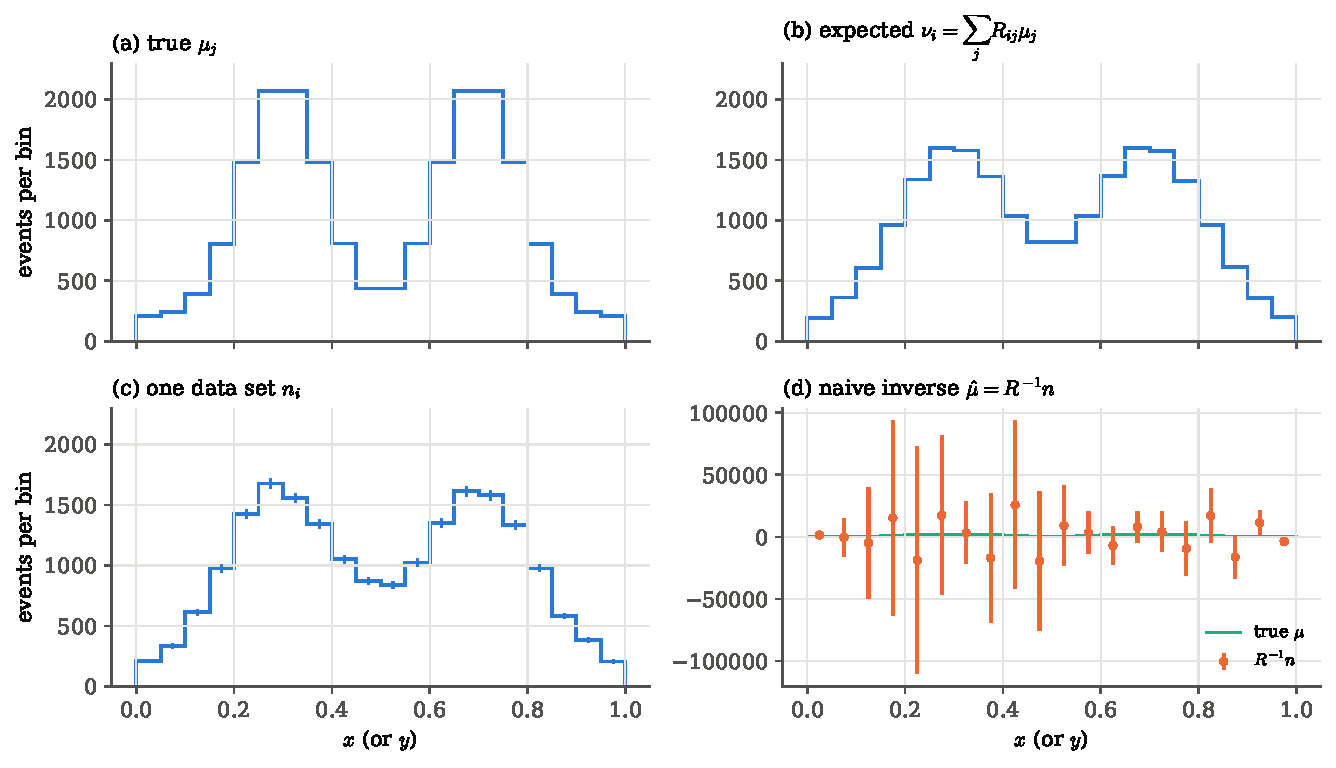
\includegraphics[width=\linewidth]{figures/ch06/unfold_inverse.pdf}
\caption{(a) The true histogram: two peaks on a flat floor. (b) What the detector makes of it on
average: the peaks are lower and broader and the dip is filled in. (c) One simulated data set,
with Poisson error bars of a few per cent. (d) The data set unfolded by inverting the response
matrix. Note the vertical scale: the estimates swing between about $\pm10^5$ and the true
histogram (green) is a thin line near zero.}
\label{6b:fig:unf-inverse}
\end{figure}

\paragraph{Why it fails: the simplest smearing first.} The failure is not a bug, and to see where
it comes from we shrink the problem to two bins \cite{HoeckerKartvelishvili1996}. Let an event
stay in its bin with probability $(1+\epsilon)/2$ and cross to the other with probability
$(1-\epsilon)/2$, with $0<\epsilon\le1$. A perfect detector has $\epsilon=1$; a detector that
can hardly tell the bins apart has $\epsilon\ll1$. No event is lost, so
\[
  \mathbf R=\frac12\begin{pmatrix}1+\epsilon&1-\epsilon\\1-\epsilon&1+\epsilon\end{pmatrix}.
\]
Which patterns does this matrix leave alone, apart from a factor? Try the sum pattern
$\bm u_+=(1,1)/\sqrt2$ and the difference pattern $\bm u_-=(1,-1)/\sqrt2$:
\begin{align}
  \mathbf R\bm u_+
  \eqby{1}\frac{1}{2\sqrt2}\begin{pmatrix}(1+\epsilon)+(1-\epsilon)\\(1-\epsilon)+(1+\epsilon)\end{pmatrix}
  =1\cdot\bm u_+ ,
  \qquad
  \mathbf R\bm u_-
  \eqby{2}\frac{1}{2\sqrt2}\begin{pmatrix}(1+\epsilon)-(1-\epsilon)\\(1-\epsilon)-(1+\epsilon)\end{pmatrix}
  =\epsilon\,\bm u_- .
  \label{6b:eq:unf-2bin-eig}
\end{align}
\begin{explain}
  \item Each component is a row of $\mathbf R$ times $(1,1)/\sqrt2$.
  \item The same with $(1,-1)/\sqrt2$.
\end{explain}
So the detector passes the total number of events unchanged (eigenvalue $1$) and multiplies the
difference between the bins by $\epsilon$ (eigenvalue $\epsilon$). Write the truth in these
patterns, $\bm\mu=s\,\bm u_++d\,\bm u_-$, with $s=(\mu_1+\mu_2)/\sqrt2$ and $d=(\mu_1-\mu_2)/\sqrt2$.
Then $\bm\nu=s\,\bm u_++\epsilon d\,\bm u_-$: the measured difference is the true difference
shrunk by $\epsilon$. Inverting means dividing the measured difference by $\epsilon$.

Now add the noise. Suppose both bins expect about $\bar\nu$ events, so that $\mathbf V\approx\bar\nu\,\Id$.
A rotation to the patterns $\bm u_\pm$ keeps this covariance as it is, so the measured sum and
measured difference, $n_s=\bm u_+\cdot\bm n$ and $n_d=\bm u_-\cdot\bm n$, each carry noise of
variance $\bar\nu$, independently. The inverse estimates $\hat s=n_s$ and $\hat d=n_d/\epsilon$, so
\begin{align}
  &\Var(\hat d)\eqby{1}\frac{\bar\nu}{\epsilon^2},
  \qquad
  \Var(\hat\mu_1)\eqby{2}\frac{\Var(\hat s)+\Var(\hat d)}{2}
  =\frac{\bar\nu}{2}\Bigl(1+\frac1{\epsilon^2}\Bigr),
  \nonumber\\
  &\rho(\hat\mu_1,\hat\mu_2)\eqby{3}\frac{\Var(\hat s)-\Var(\hat d)}{\Var(\hat s)+\Var(\hat d)}
  =\frac{\epsilon^2-1}{\epsilon^2+1}.
  \label{6b:eq:unf-2bin-var}
\end{align}
\begin{explain}
  \item Dividing by $\epsilon$ multiplies a variance by $1/\epsilon^2$.
  \item $\hat\mu_1=(\hat s+\hat d)/\sqrt2$ and $\hat s,\hat d$ are independent.
  \item $\hat\mu_2=(\hat s-\hat d)/\sqrt2$, so $\Cov(\hat\mu_1,\hat\mu_2)=(\Var\hat s-\Var\hat d)/2$;
        divide by the common variance of \textup{(2)}.
\end{explain}
Put in numbers: $\bar\nu=1000$ and $\epsilon=0.1$. Each measured bin is good to
$\sqrt{1000}\approx32$ events, but each unfolded bin has standard deviation
$\sqrt{500\times101}\approx225$, seven times worse, and the two unfolded bins are correlated with
$\rho=-0.98$. The reason is plain. With $\epsilon=0.1$ the detector shrinks a true difference of
$100$ events to a measured difference of $10$, which is smaller than the Poisson noise of that difference, $\sqrt{2\times1000}\approx45$.
The measured difference is then mostly noise, and dividing by $\epsilon$ blows that noise up ten
times and paints it back onto the two bins with opposite signs.

\paragraph{Gaussian smearing: many patterns, each shrunk.} A real detector has many bins, and
the same reasoning applies pattern by pattern. Take Gaussian smearing on a ring of $M$ bins of
width $\Delta$ (a periodic range of length $L=M\Delta$, so that no bin is at an edge), and let
$R_{ij}=r(i-j)$ depend only on how many bins the event moved, with $r(m)\approx\Delta\,g(m\Delta)$
and $g$ the Gaussian density of standard deviation $\sigma$. Which patterns does it leave alone?
On a ring every bin looks the same, so try a wave, $v_j=e^{\mathrm i q j\Delta}/\sqrt M$ with
wavenumber $q=2\pi k/L$, $k=0,1,\dots,M-1$:
\begin{align}
  (\mathbf R\bm v)_i
  \eqby{1}\sum_j r(i-j)\,\frac{e^{\mathrm i qj\Delta}}{\sqrt M}
  \eqby{2}\frac{e^{\mathrm i qi\Delta}}{\sqrt M}\sum_m r(m)\,e^{-\mathrm i qm\Delta}
  \eqby{3}v_i\int g(x)\,e^{-\mathrm i qx}\,\dd x
  \eqby{4}e^{-q^2\sigma^2/2}\,v_i .
  \label{6b:eq:unf-gauss-eig}
\end{align}
\begin{explain}
  \item Matrix times vector.
  \item Substitute $m=i-j$; on the ring $m$ runs over all $M$ shifts, and $e^{\mathrm iqj\Delta}
        =e^{\mathrm iqi\Delta}e^{-\mathrm iqm\Delta}$.
  \item $r(m)\approx\Delta\,g(m\Delta)$, and a sum of $\Delta$ times a smooth function over a
        grid of spacing $\Delta$ is its integral, with $x=m\Delta$.
  \item The Fourier transform of a Gaussian density. Complete the square as in
        \cref{1b:ex:smearing}: $-x^2/2\sigma^2-\mathrm iqx=-(x+\mathrm iq\sigma^2)^2/2\sigma^2-q^2\sigma^2/2$;
        the shifted Gaussian still integrates to one.
\end{explain}
A wave of wavenumber $q$ is passed through with its amplitude multiplied by
$\lambda_q=e^{-q^2\sigma^2/2}$. Long waves ($q\sigma\ll1$) pass almost untouched; waves shorter than
the resolution are crushed. This is the precise sense in which ``smearing removes fine
structure''. The data contain the shrunken waves plus Poisson noise, and the noise is spread
evenly over all waves: with $\mathbf V\approx\bar\nu\Id$, each wave component of $\bm n$ has variance
$\bar\nu$, as in the two-bin case. Inverting divides wave $k$ by $\lambda_k$, so using
$\mathbf R^{-1}=\sum_k\lambda_k^{-1}\bm v_k\bm v_k^\dagger$ in \eqref{6b:eq:unf-inv-cov},
\begin{equation}
  U_{jj}\eqby{1}\bar\nu\sum_k\lambda_k^{-2}\,\lvert v_{k,j}\rvert^2
  \eqby{2}\frac{\bar\nu}{M}\sum_{k}e^{q_k^2\sigma^2} .
  \label{6b:eq:unf-gauss-var}
\end{equation}
\begin{explain}
  \item $\mathbf U=\bar\nu\,\mathbf R^{-1}(\mathbf R^{-1})^\dagger=\bar\nu\sum_k\lambda_k^{-2}\bm v_k\bm v_k^\dagger$,
        because the waves are orthonormal and the $\lambda_k$ are real.
  \item $\lvert v_{k,j}\rvert^2=1/M$ for every wave, and $\lambda_k^{-2}=e^{q_k^2\sigma^2}$.
\end{explain}
The sum is dominated by the shortest wave. In our test case $\sigma=1.5\Delta$, and on an interval
with edges, rather than a ring, the natural waves are cosines with a whole number of half
wavelengths, $q_k=\pi k/L$. The shortest has $q\sigma=\pi\times19\times0.075\approx4.5$, so the
formula predicts a gain of $\SixBUfLamMinFormula$ for it. The singular values of our simulated
$\mathbf R$ (the gains of its patterns; for a symmetric matrix they are the absolute eigenvalues)
run from $\SixBUfSmax$ down to $\SixBUfSmin$, a ratio of $\SixBUfCond$, and follow the Gaussian
formula over three decades (\cref{6b:fig:unf-response}); the last few lie above it because a
finite matrix with edges is not exactly a ring. A wave that the detector shrinks to $\SixBUfSmin$ of its size must be
stretched back by the inverse of that factor, noise included. Averaged over the bins, the
standard deviation of the naive inverse is $\SixBUfRmsInv$ events for a true content of about
$1000$.

\begin{keyidea}[Why unfolding is hard]
Smearing multiplies each pattern of the true histogram by a gain $\lambda_k$ (for Gaussian
resolution $\lambda_k=e^{-q_k^2\sigma^2/2}$), small for patterns finer than the resolution. The
noise of the data is not shrunk. Inverting the response divides every pattern by its gain, so
the fine patterns of the answer are noise amplified by $1/\lambda_k$. The inverse is unbiased and
efficient, and useless whenever some gain is smaller than the relative noise.
\end{keyidea}

\begin{figure}[htbp]
\centering
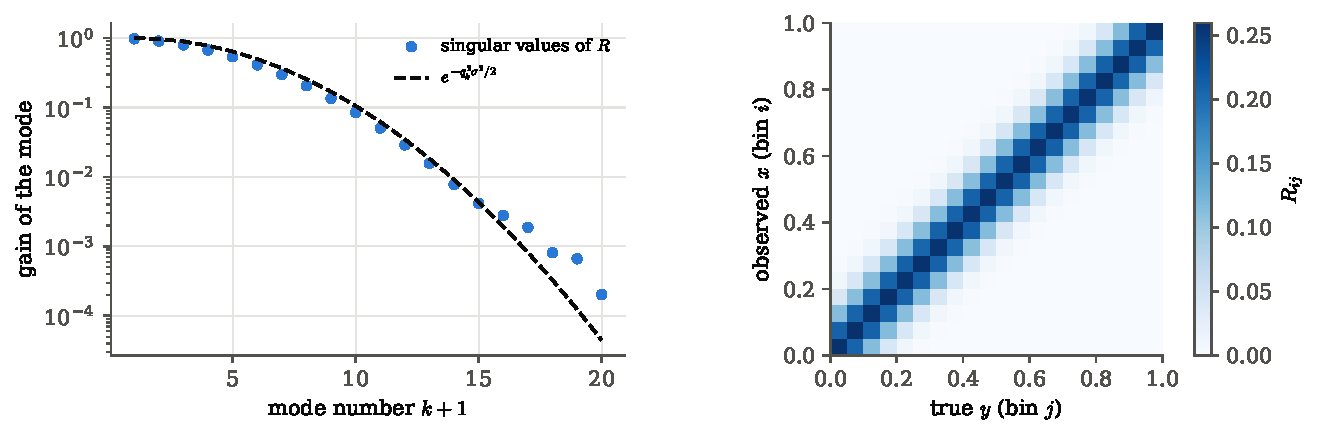
\includegraphics[width=\linewidth]{figures/ch06/unfold_response.pdf}
\caption{Right: the simulated response matrix of the test case; each column spreads the events
of one true bin over about five measured bins, and the edge columns lose events. Left: its
singular values, the factors by which it shrinks its patterns, from the smoothest to the
roughest, against the Gaussian prediction $e^{-q_k^2\sigma^2/2}$ with $q_k=\pi k/L$ (dashed).}
\label{6b:fig:unf-response}
\end{figure}

The analysis also says what helps. Wider bins remove the shortest waves from the problem
altogether, so the covariance of the inverse shrinks quickly once the bins are wider than the
resolution \srcref{Cowan}{p.~163}. And if one keeps the naive inverse, it is still an honest
result as long as the \emph{full} covariance $\mathbf U$ goes with it: a $\chi^2$ comparison with
a theory, $(\hat{\bm\mu}-\bm\mu_0)\T\mathbf U^{-1}(\hat{\bm\mu}-\bm\mu_0)$, is valid, whereas the same
$\chi^2$ with only the diagonal of $\mathbf U$ is meaningless, because the off-diagonal elements are
as large as the diagonal ones.

\subsection{Trading bias for variance: regularisation}
\label{6b:sec:unf-tikhonov}

The naive inverse is unbiased and has the smallest variance of any unbiased estimator. So any
estimator with a smaller variance must be \emph{biased}. That is the whole art of unfolding:
accept a bias that is small if some belief about the truth is right (usually, that it is
smooth) in exchange for a large cut in variance \srcref{Cowan}{\S11.4}. The tool is the
mean squared error of \cref{3a:sec:mse}, $\text{MSE}=\text{bias}^2+\text{variance}$, which
puts the two on one scale.

\paragraph{Smoothest among the acceptable.} Cowan states the strategy in two steps. First, a
whole region of true histograms fits the data acceptably: those whose log-likelihood is within
some $\Delta\ln L$ of the maximum, $\ln L(\bm\mu)\ge\ln L_{\max}-\Delta\ln L$. The naive inverse is the
single best fit, but its wild neighbours fit almost as well, which is exactly what the large
$\mathbf U$ said. Second, among the acceptable histograms, pick the smoothest, as measured by a
\newterm{regularisation function} $S(\bm\mu)$ that is larger for smoother histograms. Maximising
$S$ subject to the likelihood constraint is, with a Lagrange multiplier $\alpha$, maximising
$\alpha\ln L(\bm\mu)+S(\bm\mu)$ \srcref{Cowan}{eqs.~11.34--11.37}. A large $\alpha$ gives back the
naive inverse; $\alpha\to0$ ignores the data and returns the smoothest histogram there is.

\paragraph{Tikhonov regularisation.} The most common smoothness measure is the mean squared
curvature, Tikhonov's choice
\srcref{Cowan}{\S11.5.1}. For a histogram the second derivative becomes the second difference
$\mu_i-2\mu_{i+1}+\mu_{i+2}$, and
\begin{equation}
  S(\bm\mu)=-\sum_{i=1}^{M-2}(\mu_i-2\mu_{i+1}+\mu_{i+2})^2=-\lvert\mathbf C\bm\mu\rvert^2
  =-\bm\mu\T\mathbf G\bm\mu ,
  \qquad \mathbf G=\mathbf C\T\mathbf C ,
  \label{6b:eq:unf-curv}
\end{equation}
where row $i$ of the $(M-2)\times M$ matrix $\mathbf C$ is $(\dots,0,1,-2,1,0,\dots)$ starting in
column $i$. ($\mathbf G$ is Cowan's matrix in \srcref{Cowan}{eq.~11.48}: $6$ on most of the
diagonal, $-4$ and $1$ beside it.) A straight line has zero second differences, so
$S$ does not penalise the overall level or slope at all; those are left entirely to the data,
and a truth that is linear is unfolded without bias \srcref{Cowan}{p.~177}.

With many events per bin the Poisson log-likelihood is close to the Gaussian
$\ln L=-\tfrac12\chi^2(\bm\mu)$, $\chi^2=(\bm n-\mathbf R\bm\mu)\T\mathbf V^{-1}(\bm n-\mathbf R\bm\mu)$, taking
$\bm\beta=0$ for brevity. Maximising $\alpha\ln L+S$ is then minimising
\begin{equation}
  \chi^2(\bm\mu)+\tau\,\bm\mu\T\mathbf G\bm\mu ,
  \qquad \tau=2/\alpha ,
  \label{6b:eq:unf-tik-objective}
\end{equation}
and since this is quadratic in $\bm\mu$, the minimum has a closed form. Set the gradient to zero:
\begin{align}
  0
  &\eqby{1}-2\mathbf R\T\mathbf V^{-1}(\bm n-\mathbf R\hat{\bm\mu})+2\tau\mathbf G\hat{\bm\mu}
  \nonumber\\
  \Rightarrow\quad
  \hat{\bm\mu}_\tau
  &\eqby{2}\bigl(\mathbf R\T\mathbf V^{-1}\mathbf R+\tau\mathbf G\bigr)^{-1}\mathbf R\T\mathbf V^{-1}\,\bm n
  \equiv\mathbf A_\tau\bm n .
  \label{6b:eq:unf-tik}
\end{align}
\begin{explain}
  \item The gradient of a quadratic form: $\nabla_{\bm\mu}(\bm a-\mathbf R\bm\mu)\T\mathbf V^{-1}(\bm a-\mathbf R\bm\mu)
        =-2\mathbf R\T\mathbf V^{-1}(\bm a-\mathbf R\bm\mu)$ for symmetric $\mathbf V$, and
        $\nabla_{\bm\mu}\bm\mu\T\mathbf G\bm\mu=2\mathbf G\bm\mu$ for symmetric $\mathbf G$.
  \item Collect the terms in $\hat{\bm\mu}$ and multiply by the inverse of the bracket.
\end{explain}
At $\tau=0$ the bracket is $\mathbf R\T\mathbf V^{-1}\mathbf R$ and $\mathbf A_0=\mathbf R^{-1}$, the naive inverse. The
estimator is linear in the data, so its bias and covariance are exact, by the same two steps as
\eqref{6b:eq:unf-inv-cov}:
\begin{equation}
  \bm b_\tau=\E[\hat{\bm\mu}_\tau]-\bm\mu\eqby{1}(\mathbf A_\tau\mathbf R-\Id)\,\bm\mu ,
  \qquad
  \mathbf U_\tau\eqby{2}\mathbf A_\tau\mathbf V\mathbf A_\tau\T .
  \label{6b:eq:unf-tik-bv}
\end{equation}
\begin{explain}
  \item $\E[\mathbf A_\tau\bm n]=\mathbf A_\tau\bm\nu=\mathbf A_\tau\mathbf R\bm\mu$.
  \item Covariance of a linear map.
\end{explain}
The bias vanishes when $\mathbf A_\tau\mathbf R=\Id$, which happens only at $\tau=0$; but it also
vanishes for any truth with $\mathbf G\bm\mu=0$, the straight lines. The bias formula contains the
unknown $\bm\mu$, which is why the bias of an unfolding can be estimated but never known
\srcref{Cowan}{\S11.6}.

\paragraph{The two bins again: how regularisation filters.} Go back to the two-bin detector of
\eqref{6b:eq:unf-2bin-eig} and penalise the difference between the bins, $\tau(\mu_1-\mu_2)^2=2\tau
d^2$ (with two bins there is no curvature; the first difference plays its role). In the
patterns $\bm u_\pm$, with $\mathbf V=\bar\nu\Id$, the objective \eqref{6b:eq:unf-tik-objective} splits into
a part for $s$ and a part for $d$, and only the second is touched:
\begin{align}
  \frac{\partial}{\partial d}\Bigl[\frac{(n_d-\epsilon d)^2}{\bar\nu}+2\tau d^2\Bigr]
  &\eqby{1}-\frac{2\epsilon(n_d-\epsilon d)}{\bar\nu}+4\tau d=0
  \nonumber\\
  \Rightarrow\quad
  \hat d_\tau
  &\eqby{2}\frac{\epsilon\,n_d}{\epsilon^2+2\tau\bar\nu}
   \eqby{3}F\cdot\frac{n_d}{\epsilon},
  \qquad
  F=\frac{\epsilon^2}{\epsilon^2+2\tau\bar\nu} .
  \label{6b:eq:unf-filter}
\end{align}
\begin{explain}
  \item The measured difference is $n_d=\epsilon d+\text{noise}$, so its $\chi^2$ term is
        $(n_d-\epsilon d)^2/\bar\nu$.
  \item Solve the linear equation for $d$.
  \item Multiply and divide by $\epsilon$: the regularised estimate is the naive one, $n_d/\epsilon$,
        times a factor $F$ between $0$ and $1$.
\end{explain}
So regularisation does not smooth in some vague sense: it multiplies the badly measured pattern
by a \newterm{filter factor} $F$, and leaves the well-measured total alone. Hoecker and
Kartvelishvili show that this is the general structure \cite{HoeckerKartvelishvili1996}: after
the data are rescaled to unit errors and $\mathbf R$ is decomposed into its patterns (its singular
value decomposition), the regularised solution multiplies the $k$-th pattern of the naive inverse by
$s_k^2/(s_k^2+\tau)$, where $s_k$ is that pattern's gain. Patterns with $s_k^2\gg\tau$ pass; those with
$s_k^2\ll\tau$ are cut. It is a low-pass filter.

Which $F$ is best? With $E[n_d]=\epsilon d$ and $\Var(n_d)=\bar\nu$, the estimate $\hat d_\tau$ has
bias $(F-1)d$ and variance $F^2\bar\nu/\epsilon^2$, so
\begin{equation}
  \text{MSE}(F)\eqby{1}F^2\frac{\bar\nu}{\epsilon^2}+(1-F)^2d^2,
  \qquad
  F^\ast\eqby{2}\frac{d^2}{d^2+\bar\nu/\epsilon^2},
  \qquad
  \text{MSE}(F^\ast)\eqby{3}\frac{d^2\,\bar\nu/\epsilon^2}{d^2+\bar\nu/\epsilon^2} .
  \label{6b:eq:unf-wiener}
\end{equation}
\begin{explain}
  \item Variance plus squared bias (\cref{3a:sec:mse}).
  \item Set $\dd\,\text{MSE}/\dd F=2F\bar\nu/\epsilon^2-2(1-F)d^2$ to zero.
  \item Insert $F^\ast$; both terms share the denominator $(d^2+\bar\nu/\epsilon^2)^2$, and their
        numerators add to $d^2(\bar\nu/\epsilon^2)(d^2+\bar\nu/\epsilon^2)$.
\end{explain}
The best filter keeps the pattern in proportion to how much of it is signal: $d^2$ is the
squared size of the true pattern and $\bar\nu/\epsilon^2$ the variance of its naive estimate.
With $\bar\nu=1000$, $\epsilon=0.1$ and a true difference $\mu_1-\mu_2=200$ ($d^2=20\,000$), the naive
estimate has $\text{MSE}=10^5$ (an error of $316$ in $d$), setting the difference to zero costs
$d^2=20\,000$ (an error of $141$), and the best filter, $F^\ast=1/6$, gets the error down to $129$.
The optimum strength follows from $F^\ast$: $2\tau\bar\nu=\epsilon^2(1/F^\ast-1)$ gives $\tau^\ast=1/(2d^2)$.
It depends on the size of the true structure, which is unknown. This is why choosing $\tau$ is the
hard part of every unfolding.

\paragraph{Other smoothness measures.} The curvature is not the only choice. The entropy of the
normalised histogram, $H=-\sum_ip_i\ln p_i$ with $p_i=\mu_i/\mu_{\rm tot}$, is largest for a flat
histogram, and it counts the number of ways $\Omega=\mu_{\rm tot}!/(\mu_1!\cdots\mu_M!)$ of
distributing the events over the bins: with Stirling's $\ln m!\approx m\ln m-m$,
$\ln\Omega\approx\mu_{\rm tot}\ln\mu_{\rm tot}-\sum_i\mu_i\ln\mu_i=-\sum_i\mu_i\ln(\mu_i/\mu_{\rm tot})=\mu_{\rm
tot}H$ \srcref{Cowan}{eqs.~11.51--11.54}. Using $S=H$ is \newterm{maximum-entropy} unfolding. It
keeps every bin positive, which Tikhonov does not, and it is popular for images with sharp
features; read as a Bayesian prior $\pi(\bm\mu)\propto\Omega$ it pulls far too hard towards a flat
histogram, so in practice its strength is tuned like $\tau$. A cross-entropy relative to a
reference histogram $\bm q$ pulls towards $\bm q$ instead of towards flatness
\srcref{Cowan}{\S\S11.5.2--11.5.4}. Each choice is unbiased for a different kind of truth:
curvature for straight lines, entropy for flat histograms, cross-entropy for $\bm q$.

\subsection{Choosing the strength}
\label{6b:sec:unf-choose}

In a test case we know the truth, so the exact bias and covariance \eqref{6b:eq:unf-tik-bv} give
the exact mean squared error averaged over the bins,
$\text{MSE}(\tau)=\frac1M\sum_i\bigl(U_{\tau,ii}+b_{\tau,i}^2\bigr)$ \srcref{Cowan}{eq.~11.79}, for every
$\tau$. \Cref{6b:fig:unf-regularised}(b) shows it for our two-peak spectrum. As $\tau$ grows the
variance falls from the naive inverse's $\SixBUfMSEinv$ per bin and the squared bias rises;
their sum has a minimum at $\tau=\SixBUfTauMSE$, where the root-mean-square error per bin is
$\SixBUfRmsMin$ events: a bias of $\SixBUfBiasAtMin$ and a standard deviation of
$\SixBUfSdAtMin$. At the optimum the bias and the statistical error are about equal; that is
what an optimal trade looks like. For scale, the Poisson error of a single bin with the mean
content would be $\SixBUfRmsPoisson$. Unfolding costs information, and no method gets it back.

\pyfile[firstline=119,lastline=128,firstnumber=119]{code/ch06/30_unfolding.py}{Tikhonov
unfolding as one linear solve}

Lines 119--122 build the second-difference matrix $\mathbf C$ of \eqref{6b:eq:unf-curv} and
$\mathbf G=\mathbf C\T\mathbf C$. The function on lines 125--128 returns $\mathbf A_\tau$ of
\eqref{6b:eq:unf-tik}: line 127 forms $\mathbf R\T\mathbf V^{-1}$ for a diagonal $\mathbf V$, and line 128
solves $(\mathbf R\T\mathbf V^{-1}\mathbf R+\tau\mathbf G)\mathbf A=\mathbf R\T\mathbf V^{-1}$ rather than forming an inverse.

\paragraph{Without the truth.} A real analysis does not know $\bm\mu$, so it needs a rule that uses
the data only. Three are common. (i) \emph{Estimate the bias.} Replace $\bm\mu$ in
\eqref{6b:eq:unf-tik-bv} by the estimate itself, $\hat{\bm b}=(\mathbf A_\tau\mathbf R-\Id)\hat{\bm\mu}_\tau$, and
lower $\tau$ until the estimated biases are no longer significant compared with their own
statistical errors \srcref{Cowan}{eqs.~11.76--11.83}. (ii) \emph{The effective rank.}
Hoecker and Kartvelishvili rotate the rescaled data into the patterns of $\mathbf R$; the
coefficients fall with the pattern number until they reach the noise level, which is one. If
that happens at pattern $k$, they set $\tau=s_k^2$, so that the filter passes exactly the patterns
the data can see \cite{HoeckerKartvelishvili1996}. They also recommend checking the choice on a
test distribution close to, but different from, the simulated one, which is what our toys do.
(iii) \emph{The L-curve.} Plot, for each $\tau$, how badly the solution fits the data,
$\chi^2(\hat{\bm\mu}_\tau)$, against how rough it is, $\lvert\mathbf C\hat{\bm\mu}_\tau\rvert^2$, both on log
scales. Small $\tau$ gives tiny misfit and huge roughness, large $\tau$ the reverse, and in between
the curve turns a corner; the corner, the point of largest curvature, is the compromise. For our
one data set the corner sits at $\tau=\SixBUfTauL$, close to the minimum-MSE value
(\cref{6b:fig:unf-regularised}c).

\begin{figure}[htbp]
\centering
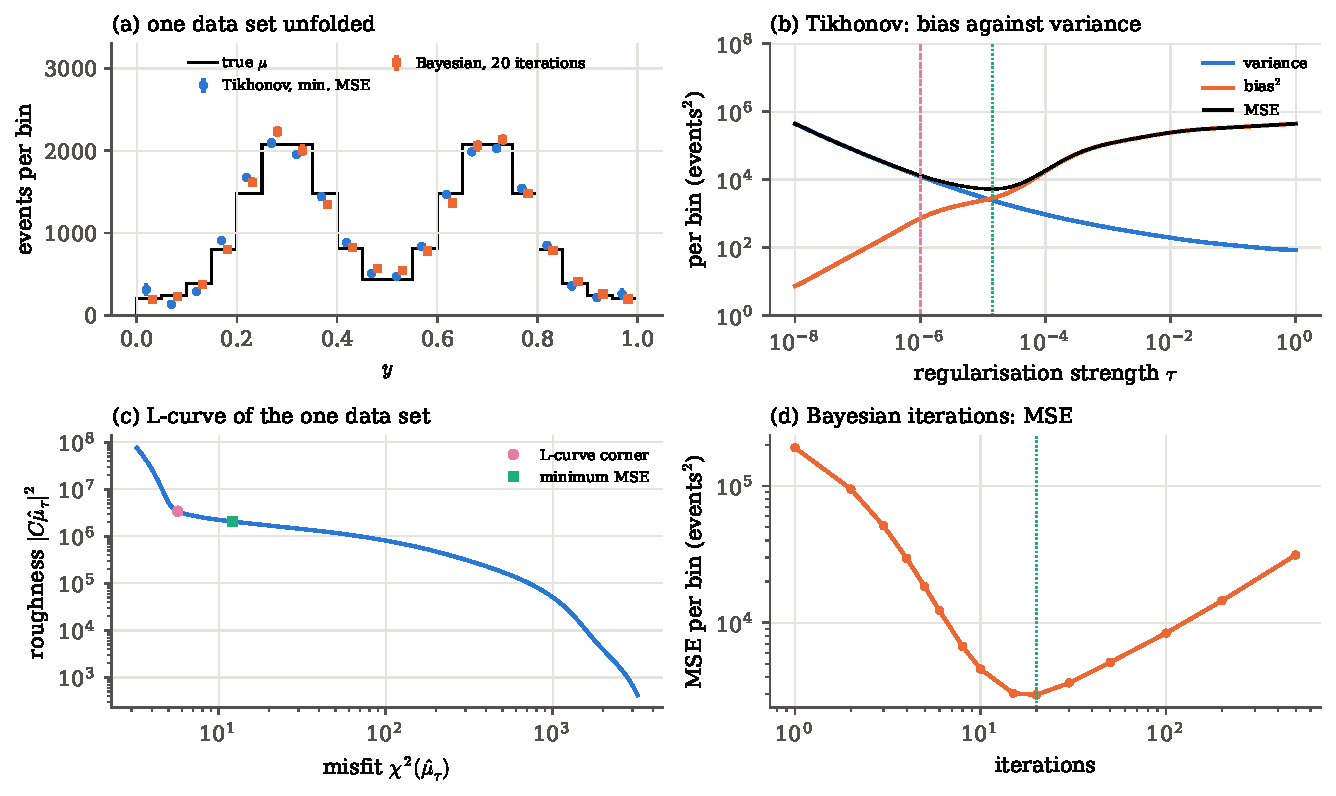
\includegraphics[width=\linewidth]{figures/ch06/unfold_regularised.pdf}
\caption{(a) The data set of \cref{6b:fig:unf-inverse} unfolded with curvature regularisation at
the minimum-MSE strength (blue) and with $\SixBUfKbest$ Bayesian iterations (orange), on the truth (black).
(b) Exact variance, squared bias and their sum, the MSE, per bin against $\tau$; the dotted line
marks the minimum, the dashed one the L-curve choice. (c) The L-curve of this data set: misfit
against roughness as $\tau$ runs from small (upper left) to large (lower right). (d) For the
Bayesian iterations, the MSE from $1000$ toys against the number of iterations.}
\label{6b:fig:unf-regularised}
\end{figure}

\subsection{Unfolding with Bayes' theorem, iterated}
\label{6b:sec:unf-bayes}

D'Agostini's method starts from a different question \cite{DAgostini1995}. \emph{The event.} An
event has been recorded in measured bin $i$. \emph{What could have produced it?} An event created
in any of the true bins $j=1,\dots,M$. These are the hypotheses. \emph{How probable was the event
under each hypothesis?} If the event was created in true bin $j$, the probability that it was
recorded and landed in bin $i$ is the response matrix element $R_{ij}$: that is exactly what
\eqref{6b:eq:unf-R} defined. \emph{Only then the priors.} Before looking at this event, the
probability that an event comes from true bin $j$ is the fraction $p_j=\mu_j/\mu_{\rm tot}$ of the
truth in that bin. We do not know it, so we start from a guess $p_j^{(0)}$, flat for instance.
\emph{Normalise.} Bayes' theorem (\cref{ch:05}) gives the probability that an event seen in bin $i$
came from true bin $j$:
\begin{equation}
  \Prob(j\given i)=\frac{R_{ij}\,p_j^{(0)}}{\sum_{l}R_{il}\,p_l^{(0)}} .
  \label{6b:eq:unf-bayes}
\end{equation}
Now share out the data. The $n_i$ events of measured bin $i$ are assigned to the true bins in these
proportions, so true bin $j$ receives $\sum_in_i\Prob(j\given i)$ recorded events. Recorded events
are only the fraction $\varepsilon_j$ of those created, so divide by the efficiency:
\begin{equation}
  \hat\mu_j^{(1)}=\frac{1}{\varepsilon_j}\sum_{i}n_i\,\Prob(j\given i)
  =\frac{\hat\mu_j^{(0)}}{\varepsilon_j}\sum_iR_{ij}\,\frac{n_i}{\hat\nu_i^{(0)}},
  \qquad \hat\nu_i^{(0)}=\sum_lR_{il}\hat\mu_l^{(0)} .
  \label{6b:eq:unf-ibu}
\end{equation}
The second form follows by inserting \eqref{6b:eq:unf-bayes} with $p_j^{(0)}=\hat\mu_j^{(0)}/\hat\mu^{(0)}_{\rm
tot}$; the total cancels between numerator and denominator. The result depends on the prior guess,
which was the weak point of a Bayesian unfolding. D'Agostini's remedy is to iterate: use
$\hat{\bm\mu}^{(1)}$ as the new prior, apply \eqref{6b:eq:unf-ibu} again, and so on.

Where do the iterations go? At a fixed point, $\hat\mu_j^{(t+1)}=\hat\mu_j^{(t)}$, the second form of
\eqref{6b:eq:unf-ibu} says
\begin{equation}
  \frac{1}{\varepsilon_j}\sum_iR_{ij}\frac{n_i}{\hat\nu_i}\eqby{1}1
  \quad\Longleftrightarrow\quad
  \sum_iR_{ij}\frac{n_i}{\hat\nu_i}\eqby{2}\sum_iR_{ij}
  \quad\Longleftrightarrow\quad
  \sum_iR_{ij}\Bigl(\frac{n_i}{\hat\nu_i}-1\Bigr)=0 ,
  \label{6b:eq:unf-fixed}
\end{equation}
\begin{explain}
  \item Divide the fixed-point condition by $\hat\mu_j$ (for a bin with $\hat\mu_j\neq0$).
  \item The efficiency is the column sum, \eqref{6b:eq:unf-eff}.
\end{explain}
which is the maximum-likelihood condition \eqref{6b:eq:unf-ml}. So iterating forever leads towards
the maximum-likelihood solution, the naive inverse whenever that is positive, with all its noise.
(The iteration is the expectation--maximisation algorithm for Poisson data, known in astronomy
as Richardson--Lucy deconvolution.) Stopping early leaves the answer between the prior guess and
the maximum-likelihood solution, and the number of iterations plays the role of $\tau$. The smooth
patterns, which have large gains, converge in a few iterations; the rough ones, with tiny gains,
would take thousands. Stopping early is therefore a filter too.

\pyfile[firstline=172,lastline=179,firstnumber=172]{code/ch06/30_unfolding.py}{Iterative
Bayesian unfolding}

Line 175 sets the starting guess: the observed total spread flat over the true bins. In each
iteration line 177 folds the current guess, $\hat\nu_i=\sum_jR_{ij}\hat\mu_j$, and line 178 is the second
form of \eqref{6b:eq:unf-ibu}. Written this way it works on a whole stack of toy data sets at once.

\paragraph{Example: how many iterations?} With $1000$ toy data sets drawn from our $\bm\nu$, the
mean squared error per bin falls steeply at first, while the iterations move the flat guess
towards the peaks, reaches its minimum of $\SixBUfMSEibu$ (an error of $\SixBUfRmsIbu$ events
per bin) at $\SixBUfKbest$ iterations, and rises again as noise creeps in: after $\SixBUfItLast$
iterations it is $\SixBUfMSEibuLast$ (\cref{6b:fig:unf-regularised}d). A small fixed number of iterations, chosen once and for all, would be far from optimal here,
because our peaks are narrow and the flat start is far from them. The right number depends on the problem, and has to be chosen with the same care
as $\tau$. The error bars of an iterative unfolding cannot be read off a formula as simply as
\eqref{6b:eq:unf-tik-bv}; we get them by unfolding $400$ Poisson resamplings of the data and taking
the spread.

\paragraph{The method of correction factors.} The simplest unfolding of all, and perhaps the most
widely used, has no matrix: multiply each measured bin by a factor from the simulation,
$\hat\mu_i=C_i(n_i-\beta_i)$ with $C_i=\mu_i^{\rm MC}/\nu_i^{\rm MC}$, the ratio of true to measured
content of bin $i$ in the simulation \srcref{Cowan}{\S11.3}. Its expectation is
$C_i\nu_i^{\rm sig}$, with $\nu_i^{\rm sig}=\nu_i-\beta_i$ the expected signal in the bin, so its bias is
\[
  b_i=\Bigl(\frac{\mu_i^{\rm MC}}{\nu_i^{\rm MC}}-\frac{\mu_i}{\nu_i^{\rm sig}}\Bigr)\nu_i^{\rm sig},
\]
zero only if the simulation has the same ratio of true to measured content as nature. When
migrations are large this fails badly. With our flat simulation $C_i\approx1$ in the interior, so the
method returns essentially the smeared histogram: the peak bins come out $\SixBUfCfBiasPeak\%$
low and the central dip $\SixBUfCfBiasDip\%$ high. The estimate is pulled towards the shape of the
simulation, which may be the very model the measurement was meant to test.

\subsection{Do the error bars cover? Toys}
\label{6b:sec:unf-coverage}

An error bar is a promise: in about $68\%$ of repeated experiments, the interval
$\hat\mu_j\pm\hat\sigma_j$ should contain the true $\mu_j$ (\cref{4b:sec:coverage}). For a regularised
unfolding the promise is in doubt, because $\hat\sigma_j$ describes only the spread of $\hat\mu_j$, not
its offset from the truth. We check it with toys, the Monte Carlo of everything in this chapter.
Draw $\SixBUfNtoy$ data sets $n_i\sim\mathrm{Poisson}(\nu_i)$ from the known truth. Unfold each one
exactly as a real analysis would, with error bars computed from that data set alone: for the naive
inverse and for Tikhonov from \eqref{6b:eq:unf-inv-cov} and \eqref{6b:eq:unf-tik-bv} with
$\mathbf V=\mathrm{diag}(\bm n)$, for the Bayesian iterations from $100$ Poisson resamplings, and for
the correction factors as $C_i\sqrt{n_i}$. Then count, bin by bin, the fraction of toys whose
interval contains $\mu_j$. The binomial error of each fraction is $\SixBUfCovSe\%$.

The naive inverse covers $\SixBUfCovInvMean\%$ of the time averaged over the bins, against the
nominal $\SixBUfNominal\%$: its enormous error bars are honest. The regularised methods do not
keep the promise (\cref{6b:fig:unf-coverage}). Tikhonov at the minimum-MSE strength covers
$\SixBUfCovTikMean\%$ on average and only $\SixBUfCovTikPeak\%$ in the bin at the top of a
peak; the worst bin reaches $\SixBUfCovTikMin\%$. The Bayesian iterations cover
$\SixBUfCovIbuMean\%$ on average, down to $\SixBUfCovIbuMin\%$ in the central dip, while the peak
bin is fine ($\SixBUfCovIbuPeak\%$). The correction factors almost never cover
($\SixBUfCovCfMean\%$): their error bars are the small Poisson errors of the data, and their bias is
tens of per cent.

\begin{figure}[htbp]
\centering
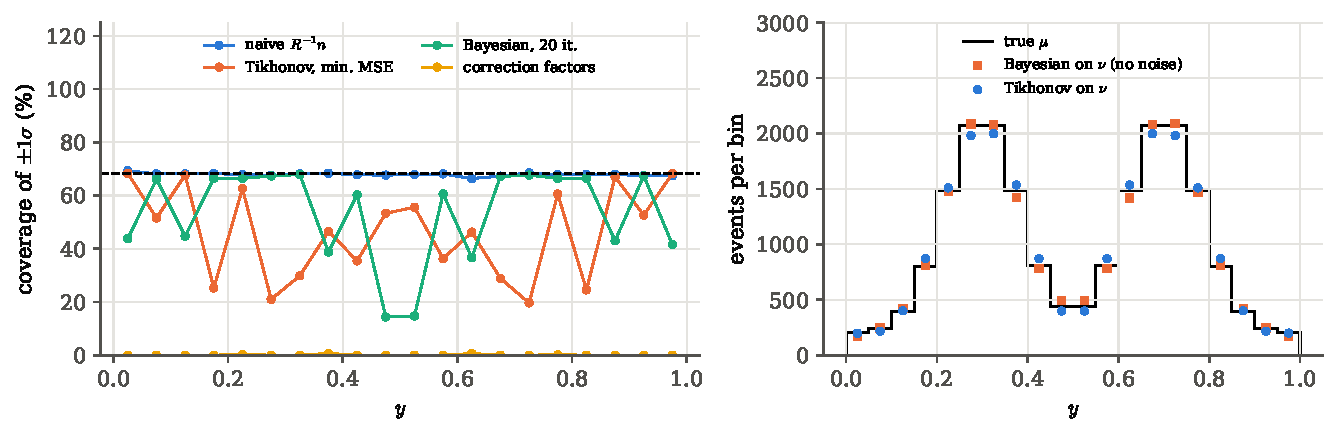
\includegraphics[width=\linewidth]{figures/ch06/unfold_coverage.pdf}
\caption{Left: the fraction of $2000$ toy experiments in which the $\pm1\sigma$ error bar of each bin
contains the true value, for four unfoldings; the dashed line is the nominal $\SixBUfNominal\%$. Right: the
two regularised methods applied to the noise-free expectation $\bm\nu$, which shows their bias
alone. Curvature regularisation shaves the peaks; the Bayesian iterations, started flat, leave
the dip partly filled.}
\label{6b:fig:unf-coverage}
\end{figure}

Why does each method fail where it does? The right panel of \cref{6b:fig:unf-coverage} unfolds the
expectation $\bm\nu$ itself, with no noise, so that only the bias is left. Each method is biased
towards what it regards as simple. The curvature penalty prefers straight lines, so it cuts the
tops of the peaks, where the curvature is largest. The Bayesian iterations remember their flat
start, so they leave too many events in the dip between the peaks. The bias is a property of the
method and the truth together, which is why it does not average away over toys and why the
coverage fails in different bins for different methods.

\begin{pitfall}[Regularised error bars are not distances to the truth]
The covariance $\mathbf A_\tau\mathbf V\mathbf A_\tau\T$ of a regularised unfolding is the spread of the
estimate about its own biased mean. Quoting it as the uncertainty on the true spectrum
undercovers: in our test case one bin is covered $\SixBUfCovTikMin\%$ of the time instead of
$\SixBUfNominal\%$. Either check the coverage with
toys and add the bias as a systematic error, or compare the theory with the data the other way
round, by folding the theory through $\mathbf R$.
\end{pitfall}

That last option is the one to prefer whenever it is possible. To test a theory, nothing needs
to be unfolded: fold the theory's prediction through the response, $\bm\nu=\mathbf R\bm\mu_{\rm
theory}+\bm\beta$, and compare it with $\bm n$ using the Poisson likelihood. That comparison is
unbiased, has the simple Poisson errors of the data, and is exactly the forward model of
\cref{1b:ex:smearing}. Unfolding earns its cost when the result must be compared with other
experiments or with theories not yet written, and then it must be published together with its
full covariance and, ideally, the response matrix itself \srcref{Cowan}{pp.~153--154}.

\begin{inpractice}[Unfolding in research]
\emph{Verification} is what our test case does: a known truth, a known detector, toys that check
the bias, the variance and the coverage of every method. \emph{Research} use looks the same with
the truth unknown. Collider experiments unfold differential cross sections (a jet's transverse
momentum, a top quark's rapidity) with a response matrix from an event generator and a
\textsc{Geant4} detector simulation (\cref{6b:sec:acceptance}), using either curvature/SVD
regularisation \cite{HoeckerKartvelishvili1996} or the iterative Bayesian method
\cite{DAgostini1995}, with the regularisation strength and the coverage checked on toys built
from alternative truths. Cosmology meets the same linear algebra: a partial-sky power spectrum is
the true $\Cell$ multiplied by a mode-coupling matrix of the mask (\cref{ch:08}), and the
pseudo-$\Cell$ method inverts that matrix only after binning in $\ell$, the ``wider bins'' cure of
\cref{6b:sec:unf-inverse}, because the unbinned matrix is as ill-conditioned as a smearing
matrix.
\end{inpractice}

\paragraph{The lesson.} Unfolding is the backward, inference direction of
a forward chain that simulation lets us write down exactly, and a measurement can only return the
patterns its detector did not crush, so every answer beyond those patterns is a choice of bias
that has to be shown, checked with toys and reported.
\section{Shrinking $\sigma$: variance reduction}
\label{6b:sec:varred}

The Monte Carlo error $\sigma/\sqrt N$ of \cref{6b:sec:sqrtN} has two factors, and only
one of them is ours to change. With independent random draws the $1/\sqrt N$ is fixed: a
hundred times the computing time buys one more digit. The constant $\sigma$, the standard
deviation of a single term, is not fixed. Importance sampling (\cref{6b:sec:importance}) changes it by moving the draws to where
the integrand lives. Three other cheap devices change it by arranging the draws more cleverly
\srcref{HobsonBMC}{\S3.1}. We test each on the same integral,
\[
  I=\int_0^1e^x\,\dd x=e-1=\SixBVrI,
\]
where plain Monte Carlo with uniform $U$ has single-term variance
$\sigma^2=\E[e^{2U}]-I^2=\tfrac12(e^2-1)-(e-1)^2=\SixBVrVarPlain$. Every estimator below uses
the same number $N$ of evaluations of $e^x$, so their variances can be compared directly.

\paragraph{The question.} Without changing the integrand or the number of function
evaluations, how can we make the average less noisy?

\subsection{Antithetic pairs}
\label{6b:sec:antithetic}

If $U$ is uniform, so is $1-U$. Evaluate the integrand at both and average the pair. Why
should this help? For a monotone integrand, a draw that lands high is paired with one that
lands low, so their errors partly cancel. To see how much, compute the variance of one
pair,
\begin{align}
  \Var\Bigl[\tfrac12\bigl(h(U)+h(1-U)\bigr)\Bigr]
  \eqby{1}\tfrac14\bigl[\Var h(U)+\Var h(1-U)+2\Cov\bigl(h(U),h(1-U)\bigr)\bigr]
  \eqby{2}\tfrac12\bigl(\sigma^2+\gamma\bigr),
  \label{6b:eq:antithetic}
\end{align}
\begin{explain}
  \item The variance of a sum of two correlated terms, with the factor $\tfrac12$ squared.
  \item $h(U)$ and $h(1-U)$ both have variance $\sigma^2$; write
        $\gamma=\Cov\bigl(h(U),h(1-U)\bigr)$.
\end{explain}
With $N$ evaluations we have $N/2$ pairs, and the average of $N/2$ independent pairs has
variance $\frac12(\sigma^2+\gamma)/(N/2)=(\sigma^2+\gamma)/N$. So the variance per
evaluation is $\sigma^2+\gamma=\sigma^2(1+\rho)$, where $\rho=\gamma/\sigma^2$ is the
correlation between the two members of a pair. A negative $\rho$ helps, and for a monotone
$h$ it is always negative, because $U$ and $1-U$ move in opposite directions. For $e^x$,
$\gamma=\E[e^Ue^{1-U}]-I^2=e-(e-1)^2=\SixBVrCovAnti$, almost $-\sigma^2$, so the variance per
evaluation drops from $\SixBVrVarPlain$ to $\SixBVrVarAntiPerEval$, a predicted gain of $31$.
The simulation, $\SixBVrR$ repeats with $N=\SixBVrN$, measures a gain of $\SixBVrGainAnti$ in
variance.

\subsection{Control variates}
\label{6b:sec:control}

Suppose a second function $c(x)$ is correlated with the integrand and has a mean $\mu_c$ we
know exactly. Estimate $I$ by averaging $h(X)-\beta\,[c(X)-\mu_c]$ instead of $h(X)$. The added
term has mean zero for every $\beta$, so the estimator stays unbiased, and its single-term
variance is
\begin{align}
  \Var\bigl[h-\beta(c-\mu_c)\bigr]
  &\eqby{1}\sigma_h^2-2\beta\Cov(h,c)+\beta^2\sigma_c^2
  \nonumber\\
  &\eqby{2}\sigma_h^2-\frac{\Cov(h,c)^2}{\sigma_c^2}
   \eqby{3}\sigma_h^2\bigl(1-\rho_{hc}^2\bigr)
  \quad\text{at}\quad\beta^*=\frac{\Cov(h,c)}{\sigma_c^2} .
  \label{6b:eq:control}
\end{align}
\begin{explain}
  \item The variance of a difference; the constant $\beta\mu_c$ does not contribute.
  \item Minimise over $\beta$: the derivative $-2\Cov(h,c)+2\beta\sigma_c^2$ vanishes at
        $\beta^*$; substitute it back.
  \item $\rho_{hc}=\Cov(h,c)/(\sigma_h\sigma_c)$ is the correlation coefficient.
\end{explain}
In words: we let the draws measure only the \emph{difference} between the integrand and a
function whose integral we already know. The better $c$ tracks $h$, the closer $\rho_{hc}^2$
is to one and the smaller the variance that is left.

For $h=e^x$ take $c(x)=x$, with $\mu_c=\tfrac12$ and $\sigma_c^2=\tfrac1{12}$ for $x$
uniform on $[0,1]$. Then $\Cov(e^U,U)=\E[Ue^U]-\tfrac12(e-1)=1-\tfrac12(e-1)=\tfrac12(3-e)$, using
$\int_0^1xe^x\dd x=\bigl[(x-1)e^x\bigr]_0^1=1$, so $\beta^*=6(3-e)=\SixBVrBeta$ and the residual
variance is $\SixBVrVarCtrl$, a predicted gain of $61$; the simulation measures
$\SixBVrGainCtrl$.

In physics the control variate is often a cheap approximation of an expensive
simulation: a parametrised detector response averaged against the full \textsc{Geant4}
simulation, or a leading-order cross section whose integral is known analytically.

\subsection{Stratified sampling}
\label{6b:sec:stratified}

Random draws clump: by chance, some parts of $[0,1]$ receive more points than others, and
this clumping is part of $\sigma$. Stratification forbids it. Cut $[0,1]$ into $K$ equal
strata, draw $N/K$ points uniformly inside each, and average the $K$ stratum averages. Why
does this lower the variance? The law of total variance \unpack{total variance $=$ mean of
the within-stratum variances $+$ variance of the stratum means} splits $\sigma^2$ into two
parts, and stratification removes the second one. With
$\mu_k$ and $\sigma_k^2$ the mean and variance of $h$ within stratum $k$,
\begin{align}
  \sigma^2\eqby{1}\frac1K\sum_{k=1}^K\sigma_k^2+\frac1K\sum_{k=1}^K(\mu_k-I)^2,
  \qquad
  \Var[\hat I_{\text{strat}}]
  \eqby{2}\frac1{K^2}\sum_{k=1}^K\frac{\sigma_k^2}{N/K}
  \eqby{3}\frac1N\Bigl[\sigma^2-\frac1K\sum_k(\mu_k-I)^2\Bigr]\le\frac{\sigma^2}N .
  \label{6b:eq:strat}
\end{align}
\begin{explain}
  \item The law of total variance, with the stratum chosen uniformly at random
        (each has probability $1/K$).
  \item $\hat I_{\text{strat}}=\frac1K\sum_k\hat\mu_k$, the strata are sampled independently, and
        each stratum mean $\hat\mu_k$ of $N/K$ draws has variance $\sigma_k^2/(N/K)$.
  \item Simplify and substitute the first equation.
\end{explain}
The variation \emph{between} strata, which plain sampling pays for through its random clumping,
is gone; only the variation within each stratum is left.

How fast does the error then fall? Take one point per stratum ($K=N$) and a smooth
integrand. Each stratum has width $1/N$, so $h$ varies across it by about $h'/N$, and
$\sigma_k^2\approx h'(x_k)^2/(12N^2)$, the variance of a uniform spread over that range. Then $\Var[\hat I_{\text{strat}}]\approx\frac1{N^2}\sum_kh'(x_k)^2/(12N^2)
\approx\int_0^1h'^2\dd x/(12N^3)$, so the error falls as $N^{-3/2}$ instead of $N^{-1/2}$. For
$e^x$, $\int_0^1e^{2x}\dd x=\tfrac12(e^2-1)$, which predicts a standard deviation
$0.516\,N^{-3/2}=1.6\times10^{-5}$ at $N=1024$; the simulation measures $\SixBVrSdStrat$, a
fitted slope of $\SixBVrStratSlope$, and a gain in variance of $\SixBVrGainStrat$ over plain
sampling. The evenly spread quasi-random (Sobol) points of \cref{6a:sec:qmc} push the same
idea into many dimensions, where a full grid of strata would again cost $n^d$ points.

\begin{figure}[htbp]
\centering
\begin{tikzpicture}[x=5.2cm,y=1.1cm,font=\small]
  \foreach \u in {0.05,0.11,0.14,0.37,0.41,0.44,0.48,0.83} \fill[formblue] (\u,2.4) circle (1.6pt);
  \draw[softgray] (0,2.4) -- (1,2.4);
  \node[anchor=east] at (-0.03,2.4) {plain};
  \foreach \u/\c in {0.08/formblue,0.23/fibreorange,0.31/tangentgreen,0.44/bdryred} {
    \fill[\c] (\u,1.2) circle (1.6pt);
    \fill[\c] ({1-\u},1.2) circle (1.6pt);
  }
  \draw[softgray] (0,1.2) -- (1,1.2);
  \node[anchor=east] at (-0.03,1.2) {antithetic};
  \foreach \k/\f in {0/0.6,1/0.2,2/0.8,3/0.4,4/0.1,5/0.7,6/0.5,7/0.3} {
    \draw[softgray] ({\k/8},-0.12) -- ({\k/8},0.12);
    \fill[formblue] ({(\k+\f)/8},0) circle (1.6pt);
  }
  \draw[softgray] (1,-0.12) -- (1,0.12);
  \draw[softgray] (0,0) -- (1,0);
  \node[anchor=east] at (-0.03,0) {stratified};
  \node[below] at (0,-0.15) {$0$}; \node[below] at (1,-0.15) {$1$};
\end{tikzpicture}
\caption{Eight evaluation points on $[0,1]$ three ways. Plain sampling can leave gaps and
clumps. Antithetic sampling pairs each $u$ with $1-u$ (same colour), so a high draw is always
balanced by a low one. Stratified sampling puts exactly one point in each of eight equal
strata (tick marks), which removes the clumping altogether.}
\label{6b:fig:strata}
\end{figure}

\pyfile[firstline=29,lastline=47,firstnumber=29]{code/ch06/29_variance_reduction.py}{Four
estimators of $\int_0^1e^x\dd x$ with the same number of function evaluations}

Each function returns $\SixBVrR$ independent estimates, one per row of random numbers, so that
the standard deviation of each estimator can be measured directly. Line 34 draws only $n/2$
uniforms and line 35 evaluates $e^x$ at $u$ and $1-u$. Line 42 subtracts the control variate
with the exact $\beta^*$ of \eqref{6b:eq:control}. Line 46 places one uniform point inside each of
the $n$ strata $[k/n,(k+1)/n)$.

\begin{figure}[htbp]
\centering
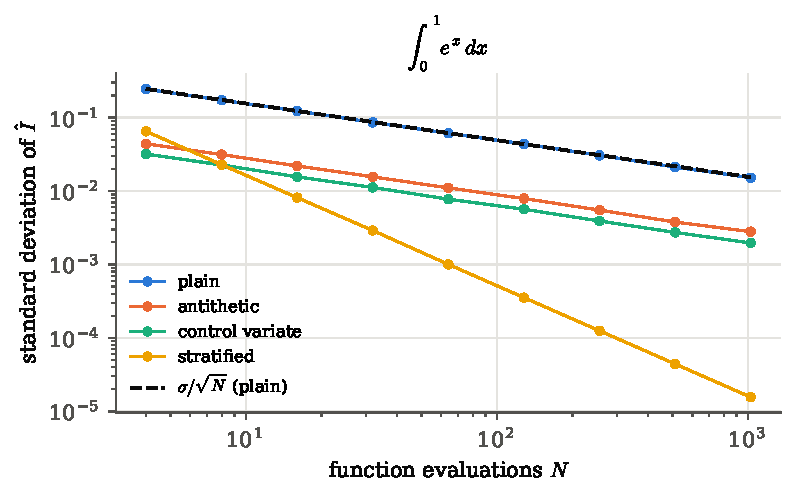
\includegraphics[width=0.62\linewidth]{figures/ch06/variance_reduction.pdf}
\caption{Standard deviation of four estimators of $\int_0^1e^x\,\dd x$ against the number of
function evaluations, each from $4000$ repeats. Plain Monte Carlo follows $\sigma/\sqrt N$
(black dashed). Antithetic pairs and the control variate keep the slope $-1/2$ but lower the line
by factors of about $5.5$ and $8$. Stratification with one point per stratum changes the slope
to $-3/2$.}
\label{6b:fig:varred}
\end{figure}

\begin{pitfall}[Error bars for correlated draws]
All three devices make the evaluations dependent: pairs are anticorrelated, strata are not
exchangeable. The naive error bar $s/\sqrt N$ computed from all $N$ values as if they were
independent is then wrong. Compute the error from the independent units: the $N/2$ pair
averages, the per-stratum variances in \eqref{6b:eq:strat}, or, as in the script, from repeated
independent runs.
\end{pitfall}

\section{Which sampler when}
\label{6b:sec:which}

The choice of sampler is usually forced by what we know about the density. Every sampler
above answers the same question, how to get draws or averages under a density we can
describe, but each asks for something different about that density.

\begin{taxonomy}[Which sampler when]
\small
\renewcommand{\arraystretch}{1.15}
\begin{tabularx}{\linewidth}{@{}>{\raggedright\arraybackslash}p{2.3cm}
                               >{\raggedright\arraybackslash}X
                               >{\raggedright\arraybackslash}p{2.6cm}
                               >{\raggedright\arraybackslash}p{2.9cm}@{}}
\toprule
method & what it needs & cost per draw & fails when\\\midrule
inverse CDF & $F^{-1}$ in closed form or fast to solve; any discrete table & one uniform & $F$ not invertible (Gaussian, most posteriors)\\
Box--Muller, polar & nothing: Gaussians & two uniforms per two normals & never; beware approximate shortcuts\\
Cholesky & covariance $\Cmat$ ($n\times n$) & $n^3/3$ once, $n^2$ per draw & $n$ large: use a diagonalising basis ($\alm$, Fourier)\\
rejection & values of $f$ up to a constant, envelope $g$, $M=\sup f/g$ & $M$ candidates & $f/g$ unbounded; high dimension ($M$ grows exponentially)\\
plain Monte Carlo integration & draws from $f$ & error $\sigma/\sqrt N$ in any dimension & $h$ concentrated where $f$ rarely goes ($\sigma$ huge)\\
importance sampling & values of $f$ (up to a constant for the self-normalised form), $g$ like $\lvert h\rvert f$ & weights $f/g$ & $g$ thinner-tailed than $f$ (infinite variance)\\
variance reduction & structure: monotone $h$, known $\int c$, smoothness & same $N$, smaller $\sigma$ & error bars computed as if draws were independent\\
MCMC (\cref{ch:09}) & values of $f$ up to a constant, nothing else & correlated draws & poor mixing, multimodality\\
\bottomrule
\end{tabularx}
\end{taxonomy}

Going down the table, we need to know less and less about $f$, until
Markov chain Monte Carlo needs only the ratio of $f$ at two points, which is the posterior
without its evidence (\cref{ch:05}). The price is that the draws become correlated, and the
$1/\sqrt N$ law then holds with $N$ replaced by an effective number of independent draws
\srcref{Lambert}{\S12.2}.

\begin{recap}
\begin{itemize}[itemsep=1pt,leftmargin=1.2em]
  \item $F(X)$ is uniform for any continuous $X$; so $X=F^{-1}(U)$ has CDF $F$. Decay times:
        $-\tau\ln(1-U)$. Power laws, isotropic directions and discrete tables follow the same way.
  \item Two uniforms give two exact Gaussians (Box--Muller): $R^2=-2\ln U_1$ is exponential and
        the angle is uniform, by the polar Jacobian. $\bm\mu+\mathbf L\bm z$ with
        $\mathbf L\mathbf L\T=\Cmat$ gives any Gaussian vector.
  \item Rejection: points uniform under $Mg$ and kept under $f$ are exact draws from $f$;
        acceptance $1/M$, geometric number of trials; needs $f/g$ bounded.
  \item An integral is an expectation; its Monte Carlo estimate has error $\sigma/\sqrt N$ in
        any dimension, beating grids ($N^{-2/d}$) above about four dimensions. The acceptance of
        a detector is the verified example; with a dead region the simulation is the answer.
  \item Importance sampling reweights by $f/g$; its variance contains $\int h^2f^2/g$, so $g$
        must have thicker tails than $f$. Self-normalised weights handle unnormalised
        posteriors.
  \item A histogram of samples estimates the bin-averaged density with binomial error
        $\sqrt{Np_k(1-p_k)}/(N\Delta)$; the oscillator at random times reproduces the arcsine
        density.
  \item Unfolding: the measured histogram is $\bm\nu=\mathbf R\bm\mu+\bm\beta$ with
        $R_{ij}=\Prob(\text{observed }i\given\text{true }j)$ from simulation. The inverse
        $\mathbf R^{-1}\bm n$ is unbiased but divides each pattern by its gain
        ($e^{-q^2\sigma^2/2}$ for Gaussian smearing), so its variance explodes. Tikhonov curvature
        and iterated Bayes trade bias for variance; choose the strength by MSE or the L-curve, and
        check the coverage with toys.
  \item Antithetic pairs, control variates and stratification shrink $\sigma$ at fixed $N$.
\end{itemize}
\end{recap}

\subsection*{Reading the literature}
\label{6b:sec:reading-list}

\begin{itemize}[itemsep=2pt,leftmargin=1.2em]
  \item \textbf{The main line.} Wasserman, \emph{All of Statistics}, Chapter~24: basic Monte
        Carlo integration, importance sampling with the tail rule, and the start of MCMC
        \mainref{pp.~403--416}; Section~11.4 on simulating the posterior \mainref{p.~180}.
  \item \textbf{The physicist's chapter.} Cowan, \emph{Statistical Data Analysis}, Chapter~3:
        uniform generators, the transformation method, acceptance--rejection, the $1/\sqrt n$
        argument against quadrature, event generators and detector simulation.
  \item \textbf{Derivations.} Casella and Berger, \emph{Statistical Inference}, Section~5.6:
        the probability integral transform, Box--Muller, discrete generation, the Accept/Reject
        theorem with its proof and the geometric number of trials.
  \item \textbf{Why sampling.} Lambert, \emph{A Student's Guide to Bayesian Statistics},
        Chapter~12 (the intractable denominator, grids, quadrature, independent sampling);
        Kruschke, \emph{Doing Bayesian Data Analysis}, Section~7.1 (a distribution represented
        by a representative sample); Hobson et al.\ (eds.), \emph{Bayesian Methods in
        Cosmology}, Chapter~3 (Monte Carlo methods for parameter estimation).
  \item \textbf{Generators.} Marsaglia on the lattice structure of congruential generators
        \cite{Marsaglia1968}; L'Ecuyer on combined and well-chosen LCGs \cite{LEcuyer1988,LEcuyer1999};
        the Mersenne Twister \cite{MatsumotoNishimura1998}; xorshift \cite{Marsaglia2003};
        PCG \cite{ONeill2014}; counter-based generators \cite{Salmon2011}; the TestU01 battery
        \cite{LEcuyerSimard2007}; Sobol's sequences \cite{Sobol1967}.
  \item \textbf{Sampling methods and physics codes.} Box and Muller \cite{BoxMuller1958};
        Marsaglia and Bray's polar method \cite{MarsagliaBray1964}; the \textsc{Pythia}~8.3 manual
        \cite{Pythia83} and the \textsc{Geant4} toolkit paper \cite{Geant4} for sampling at the
        scale of a collider experiment; Metropolis et al.\ \cite{Metropolis1953} for where
        \cref{ch:09} goes next.
\end{itemize}

\section*{Chapter summary}
\addcontentsline{toc}{section}{Chapter summary}
\label{6b:sec:summary}

Turning a probability model into numbers takes three pieces of machinery. First, uniform
numbers: a computer is deterministic, so its ``random'' numbers are the output of a finite
machine, and they must be tested like any other null hypothesis. Second, transformations:
given good uniform numbers, a few exact transformations turn them into draws from any
distribution we can describe. Third, averages: averages over those draws give integrals,
with an error $\sigma/\sqrt N$ that does not depend on the dimension. In the pipeline from
physical model to inference,
\[
  \text{physical model}\to\text{field or dataset}\to\text{summary }S\to
  \boxed{P(S\given\theta)}\to\text{infer physics},
\]
Monte Carlo is the arrow into the sampling distribution: whenever the algebra of
\cref{ch:02,ch:03} gives out, we simulate the experiment many times and histogram the summary.
\Cref{ch:07,ch:08} do this for fields and CMB maps, and \cref{ch:09} adapts it to densities
we can only evaluate.

\begin{center}
\small
\renewcommand{\arraystretch}{1.15}
\begin{tabularx}{\linewidth}{@{}>{\raggedright\arraybackslash}p{3.3cm}
                               >{\raggedright\arraybackslash}X
                               >{\raggedright\arraybackslash}p{2.5cm}@{}}
\toprule
\multicolumn{3}{@{}l}{\textbf{Random numbers on a deterministic machine}}\\
concept & operational meaning & used later in\\\midrule
Monty Hall as a test of the generator & The observed event is ``Monty opened $C$''. What made him open that door? The possible hypotheses are the three locations of the car, $H_A,H_B,H_C$. Under each we find the probability that Monty opens $C$: $\tfrac12$ under $H_A$ (he may open either goat door and tosses a coin), $1$ under $H_B$ (he must not open our door $A$ and must not reveal the car), $0$ under $H_C$ (the car is there). Only then come the priors ($\tfrac13$ each) and the normalisation, which give posterior probabilities $\tfrac13,\tfrac23,0$. A simulation reproduces this only if its coin is fair, because a biased coin changes the probability of the event under $H_A$ & every chapter\\
pseudorandom generator & a finite state, a transition function, an output function and a seed; reproducible, eventually periodic & every simulation\\
linear congruential generator & $x_{n+1}=(ax_n+c)\bmod m$; period at most $m$; low bits of a power-of-two modulus are poor & legacy codes\\
lattice structure, spectral test & $t$-tuples of an LCG lie on a lattice of parallel planes (RANDU: 15 planes in 3-D); the spectral test measures the largest gap between planes & \cref{ch:07,ch:08}\\
modern generators & bigger state and a nonlinear output function: xorshift, Mersenne Twister, PCG64 (numpy default), counter-based & every chapter\\
seeds and streams & SeedSequence hashes job identifiers into well-separated states; one stream per parallel job, never ``seed $=$ job number'' by hand & \cref{ch:08,ch:09}\\
randomness tests & each test is a null hypothesis ``the stream is i.i.d.\ uniform'': $\chi^2$ on histograms, serial correlation, runs; batteries such as TestU01 & \cref{ch:04}\\
quasi-random points & Sobol sequences fill the cube evenly; integration error close to $1/N$ instead of $1/\sqrt N$ for smooth integrands & \cref{ch:10}\\
\bottomrule
\end{tabularx}
\end{center}

\begin{center}
\small
\renewcommand{\arraystretch}{1.15}
\begin{tabularx}{\linewidth}{@{}>{\raggedright\arraybackslash}p{3.3cm}
                               >{\raggedright\arraybackslash}X
                               >{\raggedright\arraybackslash}p{2.5cm}@{}}
\toprule
\multicolumn{3}{@{}l}{\textbf{From uniform numbers to any distribution}}\\
concept & operational meaning & used later in\\\midrule
probability integral transform & $F(X)\sim\mathrm{Uniform}(0,1)$ for continuous $X$; $F^{-1}(U)$ has CDF $F$ & \cref{ch:04,ch:08}\\
inverse-CDF sampling & solve $F(x)=u$: decay times $-\tau\ln(1-u)$, power laws, isotropic directions ($\cos\theta=2u-1$), discrete tables by cumulative sums & every simulation\\
Box--Muller, polar method & $R=\sqrt{-2\ln U_1}$, $\Theta=2\pi U_2$ give two exact independent normals; the polar form keeps a fraction $\pi/4$ & \cref{ch:07,ch:08,ch:09}\\
Cholesky colouring & $\bm\mu+\mathbf L\bm z$ with $\mathbf L\mathbf L\T=\Cmat$ has covariance $\Cmat$; for isotropic fields the factor is $\sqrt{\Cell}$ per mode & \cref{ch:07,ch:08,ch:10}\\
rejection sampling & keep $V\sim g$ if $U\,Mg(V)<f(V)$; acceptance $1/M$; trials geometric; needs $f/g$ bounded; hopeless in high dimension & \cref{ch:09}\\
\bottomrule
\end{tabularx}
\end{center}

\begin{center}
\small
\renewcommand{\arraystretch}{1.15}
\begin{tabularx}{\linewidth}{@{}>{\raggedright\arraybackslash}p{3.3cm}
                               >{\raggedright\arraybackslash}X
                               >{\raggedright\arraybackslash}p{2.5cm}@{}}
\toprule
\multicolumn{3}{@{}l}{\textbf{Integrals, errors and densities from samples}}\\
concept & operational meaning & used later in\\\midrule
Monte Carlo integration & write $I=\E_f[h]$, average $h$ over draws from $f$, report $\hat I\pm s/\sqrt N$ & every chapter\\
$1/\sqrt N$ law & $\Var\hat I=\sigma^2/N$ from independence, Gaussian by the CLT; the rate is dimension-independent, the constant $\sigma$ is not; grids lose above $d\approx4$ & \cref{ch:08,ch:09,ch:10}\\
probability as a mean of an indicator & simulate and count; binomial error $\sqrt{p(1-p)/N}$ (acceptance, $\Phi(2)$, $p$-values by simulation) & \cref{ch:04,ch:08}\\
verification vs research & detector acceptance: the simulation checks $\Omega/4\pi$, then is the answer with a dead strip; event generators and detector simulation & \cref{ch:08}\\
importance sampling & average $hf/g$ over draws from $g$; variance $\int h^2f^2/g-I^2$; $g$ must have thicker tails than $f$; effective sample size $(\sum w)^2/\sum w^2$ & \cref{ch:09}\\
self-normalised weights & posterior averages $\sum\theta_jw_j/\sum w_j$ with $w=\Like\pi/g$; the evidence cancels; reweighting of simulated events & \cref{ch:09}\\
histogram as density & $n_k/(N\Delta)$ estimates the bin average $p_k/\Delta$ with error $\sqrt{Np_k(1-p_k)}/(N\Delta)$; oscillator position from random times; summaries (mode, HDI) from draws & \cref{ch:07,ch:09,ch:12}\\
variance reduction & antithetic pairs $\sigma^2(1+\rho)$, control variates $\sigma^2(1-\rho^2)$, stratification removes between-strata variance ($N^{-3/2}$ for smooth $h$) & \cref{ch:08}\\
\bottomrule
\end{tabularx}
\end{center}
  